\documentclass[12pt]{article}
\usepackage[utf8]{inputenc}
\usepackage{amsmath}
\usepackage{graphicx}
\usepackage{listings}
\usepackage{verbatim}
\usepackage{float}
\usepackage{xcolor}
\usepackage{subcaption}
\usepackage[english]{babel}
\usepackage{caption}
\usepackage{hyperref}
\usepackage{biblatex}
\addbibresource{report.bib}
\usepackage{setspace}
\usepackage{wrapfig}
\usepackage{lipsum}
\usepackage{amssymb}
\linespread{1.25}
\usepackage[a4paper, total={6in, 9in}]{geometry}
\DeclareMathOperator*{\E}{\mathbb{E}}


\hypersetup{
    colorlinks,
    linkcolor={red!50!black},
    citecolor={blue!50!black},
    urlcolor={blue!80!black}
}
\definecolor{codegreen}{rgb}{0,0.6,0}
\definecolor{codegray}{rgb}{0.5,0.5,0.5}
\definecolor{codepurple}{rgb}{0.58,0,0.82}
\definecolor{backcolour}{rgb}{0.95,0.95,0.92}
\definecolor{dkgreen}{rgb}{0,0.6,0}
\definecolor{gray}{rgb}{0.5,0.5,0.5}
\definecolor{mauve}{rgb}{0.58,0,0.82}

\lstdefinestyle{mystyle}{
    backgroundcolor=\color{backcolour},
    commentstyle=\color{codegreen},
    keywordstyle=\color{magenta},
    numberstyle=\tiny\color{codegray},
    stringstyle=\color{codepurple},
    basicstyle=\ttfamily\footnotesize,
    breakatwhitespace=false,
    breaklines=true,
    captionpos=b,
    keepspaces=true,
    numbers=left,
    numbersep=5pt,
    showspaces=false,
    showstringspaces=false,
    showtabs=false,
    tabsize=2
}

\lstset{style=mystyle}
\title{Project 1\\ Regression analysis and resampling methods}
\author{Filip Severin von der Lippe}
\date{\today}
\begin{document}
\maketitle
\begin{abstract}
  Abstract
\end{abstract}
\newpage
\tableofcontents
\section{Introduction}
In this project we will study the Franke function and real topography data by using regression analysis and resampling methods. These are both two dimensional systems which gives us a way of generalizing our functions to work for both. We will use ordinary least squares, ridge and lasso regression in our study of our data and do comparisons to try finding the optimal model for the different datasets.
\section{Method}
Our fist step is to set up our data for analysis. We start by implementing the Franke function which is a sum of four exponentials:
\begin{align*}
  f(x,y) &= \frac{3}{4 }\exp\left(- \frac{(9x -2 )^2}{4} - \frac{(9y-2)^2}{4}\right) +\frac{3}{4}\exp{\left(-\frac{(9x+1)^2}{49}- \frac{(9y+1)}{10}\right)} \\
&+\frac{1}{2}\exp{\left(-\frac{(9x-7)^2}{4} - \frac{(9y-3)^2}{4}\right)} -\frac{1}{5}\exp{\left( -(9x-4)^2 - (9y-7)^2\right) }
\end{align*}
By using this function we generate our data by using ($n+1\times n+1$) points in a meshgrid for $x$ and $y$ in the interval [0,1]. This gives us a function value of ($n+1 \times n+1$) to which we add a stochastic noise $\epsilon \sim N(0,\sigma^2)$ for a chosen standard deviation $\sigma$. This leaves us with our data described by the franke function plus some noise $\epsilon$:
\begin{align*}
  \boldsymbol{z} = f(\boldsymbol{x}) + \boldsymbol{\epsilon}
\end{align*}
This can also be assumed of some real data, for the assumtion of the existence of a continous function $f$ and normal distributed error $\epsilon$.

The ordinary least squares gives us an aproximation to the above equation where we minimize $(\boldsymbol{z} - \boldsymbol{\tilde{z}})^2$ to give us the matrix equation:
\begin{align*}
  \boldsymbol{\tilde{z}} = \boldsymbol{X}\boldsymbol{\beta}
\end{align*}
for a chosen design matrix $\boldsymbol{X}$ of some degree $n$.

This approximation gives us a new way of describing our dataset in terms of $\boldsymbol{\tilde{z}}$ instead of $f(\boldsymbol{x})$.
\begin{align*}
  \boldsymbol{z} = \sum_{j=0}^{n-1}\beta_jx_i^j + \epsilon_i
\end{align*}
This is the same as the following matrix equation:
\begin{align*}
  \boldsymbol{z} = \boldsymbol{X}\boldsymbol{\beta} + \boldsymbol{\epsilon} = \boldsymbol{\tilde{z}} + \boldsymbol{\epsilon}
\end{align*}
This means that the elemnt $i$ is given by:
\begin{align*}
  z_i = \epsilon_i + \sum_j x_{ij}\beta_j
\end{align*}
and the expectation value of the element $i$ in $\boldsymbol{z}$:
\begin{align*}
  E(z_i) = E(\epsilon_i + \sum_j x_{ij}\beta_j)
\end{align*}
Since we already know or have assumed that $\boldsymbol{\epsilon}$ is normal distibuted with the expectation value 0 $E(\epsilon_i)=0$, this gives us:
\begin{align*}
  E(z_i) = E(\epsilon_i) + E(\sum_j x_{ij}\beta_j) = \sum_jE(x_{ij}\beta_j)
\end{align*}
$x_{ij}$ and $\beta_j$ are values and not distrubutions which means they have themselves as expectation values:
\begin{align*}
    E(z_i) = \sum_jx_{ij}\beta_j = \boldsymbol{X_i}_*\boldsymbol{\beta}
\end{align*}
To find the variance we again recognize that $\boldsymbol{X}\boldsymbol{\beta}$ follow no distribution which leaves us with the variance of $\boldsymbol{z}$ equaling the variance of $\boldsymbol{\epsilon}$ which is given as $\sigma^2$:
\begin{align*}
  \text{Var}(\boldsymbol{z}) = \text{Var}(\boldsymbol{X}\boldsymbol{\beta} + \boldsymbol{\epsilon}) = \text{Var}(\boldsymbol{\epsilon}) = \sigma^2
\end{align*}
$\boldsymbol{\tilde{z}}$ is defined through the minimization of the mean square error $(\boldsymbol{z} - \boldsymbol{\tilde{z}})^2$ which for $\boldsymbol{\tilde{z}} = \boldsymbol{X}\boldsymbol{\beta}$ translates to the minimization of the cost function:
\begin{align*}
  C(\boldsymbol{\beta}) = \frac{1}{ n}\{(\boldsymbol{z}- \boldsymbol{X}\boldsymbol{\beta}^T\boldsymbol{z}- \boldsymbol{X}\boldsymbol{\beta})\}
\end{align*}
Where we take the derivative with respect to $\boldsymbol{\beta}$ and solve where the derivative is 0 to find the minimum:
\begin{align*}
  \frac{\partial C(\boldsymbol{\beta})}{\partial \boldsymbol{\beta}} = \boldsymbol{X}^T (\boldsymbol{z}- \boldsymbol{X}\boldsymbol{\beta}) =0
\end{align*}
\begin{align*}
  \boldsymbol{X}^T\boldsymbol{z} = \boldsymbol{X}^T \boldsymbol{X}\boldsymbol{\beta}
\end{align*}
We assume that $\boldsymbol{X}^T\boldsymbol{X}$ is invertible which gives us the the optimal $\boldsymbol{\beta}$:
\begin{align*}
  \boldsymbol{\tilde{\beta}} = (\boldsymbol{X}^T\boldsymbol{X})^{-1} \boldsymbol{X}^T\boldsymbol{z}
\end{align*}
We can now find the expectation value for the optimal $\boldsymbol{\tilde{\beta}}$:
\begin{align*}
  E(\boldsymbol{\tilde{\beta}}) &= E[(\boldsymbol{X}^T\boldsymbol{X})^{-1} \boldsymbol{X}^T\boldsymbol{z}] = E[(\boldsymbol{X}^T\boldsymbol{X})^{-1} \boldsymbol{X}^T(\boldsymbol{X}\boldsymbol{\beta} + \boldsymbol {\epsilon} )] \\
  &=  (\boldsymbol{X}^T\boldsymbol{X})^{-1} \boldsymbol{X}^TE[(\boldsymbol{X}\boldsymbol{\beta} + \boldsymbol {\epsilon} )] \\ &= (\boldsymbol{X}^T\boldsymbol{X})^{-1} \boldsymbol{X}^T\boldsymbol{X}\boldsymbol{\beta} \\&=  \boldsymbol{\beta}
\end{align*}
Here we see that the expectation value of our optimal parameter is the parameter $\boldsymbol{\beta}$.

We now find the variance of the optimal parameter:
\begin{align*}
  \text{Var}(\boldsymbol{\tilde{\beta}}) &= \text{Var}[(\boldsymbol{X}^T\boldsymbol{X})^{-1} \boldsymbol{X}^T(\boldsymbol{X}\boldsymbol{\beta} + \boldsymbol {\epsilon} )] \\
  &= \text{Var}[(\boldsymbol{X}^T\boldsymbol{X})^{-1} \boldsymbol{X}^T\boldsymbol {\epsilon} ]
\end{align*}
For a matrix $A$ we have Var$(\boldsymbol{AX}+b) = \boldsymbol{A}\text{Var}(\boldsymbol{X})\boldsymbol{A}^T$ which gives us:
\begin{align*}
  \text{Var}(\boldsymbol{\tilde{\beta}})&=(\boldsymbol{X}^T\boldsymbol{X})^{-1}\boldsymbol{X}^T\text{Var}[ {\boldsymbol{\epsilon}} ]((\boldsymbol{X}^T\boldsymbol{X})^{-1})^T\boldsymbol{X} \\  &=
  (\boldsymbol{X}^T\boldsymbol{X})^{-1}\boldsymbol{X}^T\text{Var}[ {\boldsymbol{\epsilon}} ](\boldsymbol{X}^T)^{-1}\boldsymbol{X}^{-1}\boldsymbol{X} \\&=
   (\boldsymbol{X}^T\boldsymbol{X})^{-1}\text{Var}[ {\boldsymbol{\epsilon}} ]
\end{align*}

This we can use to compute the optimal $\beta$ and in turn give us a OLS prediction for our real function $f$.

\subsection{Splitting and scaling of data}
A central part of regression analysis is to scale and split our data to avoid both overfitting and avoid the MSE to contain the intercept. In our case of the Franke function we have $x,y \in [0,1]$ and follwing $z$ data on the same order which may indicate that a scaling is unessecary. This expectation comes from that our data does not include any extreme values of any other order that may greatly negativly incluence our predictors. In other words scaling of data is normaly what we do to get the data as equal to each other as our Franke data already is. To test if this expectation is valid, we test this and compare our non-scaled data to mean scaled data where we have subtracted the mean.

To avoid overfitting we perform a 80-20 percent split into train and test data. We use the train data to train the model or in other words find the $\beta$ parameters. To predict we use the trained model together with the test data which leaves us with a more generalized prediction not only working for the data we have at hand, but also other data coming from the same source. This can be explained by for example a model trained so well with a design matrix $\boldsymbol{X}$ of an infinite degree that its prediction follows every noisy outlier. This woulds match the data at hand very well and give us an extremly low MSE, but give us high MSE for new data which were not used to train the model. To test this we look at both MSE and R squared for predictions for $\boldsymbol{X}$ of different degrees using only train data compared to predictions made using both train and test data.

\subsection{Mean squared error and R squared}
For different design matrices $X$ with different polynomial degrees we can calculate the mean squared error and R squared. This is done using the following equations where we define $z$ as our test data containing $n+1$ points.
\begin{align*}
  MSE(\boldsymbol{z}, \boldsymbol{\tilde{z}}) = \frac{1}{n }\sum_{i=0}^{n}(z_i- \tilde{z}_i)^2
\end{align*}
\begin{align*}
  R^2(\boldsymbol{z}, \boldsymbol{\tilde{z}}) = 1 - \frac{\sum_{i=0}^{n}(z_i- \tilde{z}_i)^2}{\sum_{i=0}^{n}(z_i- \bar{z}_i)^2}
\end{align*}
For the mean value:
\begin{align*}
  \bar{z} = \frac{1}{n }\sum_{i=0}^{n}z_i
\end{align*}

\subsection{Bias-variance trade-off}
To study the bias-variance trade-off we first implement the bootstrap resampling technique. This is done by resampling our train data $n_B$ times with replacement. That means we gain $n_B$ new samples that may be unique but still only contain values from the original sample. This in turn is used to compute our predictions leaving us with a total of $n_B$ different predictions. This can be used to study the bias and variance of the predictions.

By looking back at the cost function which is minimized in order to find our optimal parameters $\boldsymbol{\beta}$ we can derive an expression for the bias and variance.
\begin{align*}
  C(\boldsymbol{X}, \boldsymbol{\beta}) = \frac{1 }{n }\sum_ {i=0}^{n-1}(z_i - \tilde{z}_i)^2 = \E[(\boldsymbol{z}- \boldsymbol{\tilde{z}})^2]
\end{align*}
By the definition of our data $z = f +\epsilon$ we rewrite the costfunction:
\begin{align*}
  \E[(\boldsymbol{z}- \boldsymbol{\tilde{z}})^2] &= \E[(f + \epsilon - \tilde{z} + \E[\tilde{z}]- \E[\tilde{z}])^2] \\                                             &= \E[f^2 + \epsilon^2 + \tilde{z}^2 + 2\E[\tilde{z}]^2 \\
                                                 &+ 2f\epsilon + 2f\tilde{z} + 2f\E[\tilde{z}] - 2f\E[\tilde{z}]\\
                                                 &+ 2\epsilon\tilde{z} + 2\epsilon \E[\tilde{z}] - 2\epsilon \E[\tilde{z}]\\
                                                 &+ 2\tilde{z}\E[\tilde{z}] - 2\tilde{z}\E[\tilde{z}] -2\E[\tilde{z}]^2]\\
                                                 &= \E[(f-\E[\Tilde{z}])^2] + \E[\epsilon^2] + \E[( \E[\Tilde{z}] - \Tilde{z} )^2] \\
                                                 &+ 2(f-\E[\tilde{z}])\E[\epsilon]+2\E[\epsilon]\E[(\E[\tilde{z}]-\tilde{z} )] \\
                                                &+ 2(f-\E[\tilde{z}])\E[( \E[\tilde{z}] - \tilde{z} )]
\end{align*}
By using that $\epsilon \sim N(0,1)$ we have $\E[\epsilon] = 0$ and Var$[\epsilon] = \E[\epsilon^2]- \E[\epsilon]^2 = \E[\epsilon^2]=\sigma^2$ from this we get:
\begin{align*}
  \E[(\boldsymbol{z}- \boldsymbol{\tilde{z}})^2] &=\E[(f -\E[\tilde{z}])^2] +\E[( \tilde{z} -\E[\tilde{z}])^2]  + \sigma^2+ 2(f-\E[\tilde{z}])\E[\E[\tilde{z}] -\tilde{z}]\\
  &=\E[(f -\E[\tilde{z}])^2]  + \E[( \tilde{z} -\E[\tilde{z}])^2]+\sigma^2\\
  &= \E[(f -\E[\tilde{z}])^2]  + \text{var}[\tilde{f}] + \sigma^2
\end{align*}
We see that the first term is (Bias$[\tilde{f}])^2$ but we are left with a problem to compute it because $f$ is unknown. To be able to find the bias we look at the computeable $E[(y - \E[\tilde{y}])^2]$ and the relation $z= f + \epsilon$:
\begin{align*}
  E[(y - \E[\tilde{y}])^2] &= \E[(\epsilon + f - \E[\tilde{y}])^2] \\
                           &= \E[\epsilon^2] + \E[(f- \E[\tilde{y}])^2] + \E[-2\epsilon(f- \E[\tilde{y}])] \\
\end{align*}
We recognize once again that we can remove terms that have $\epsilon$ in them from $\E[\epsilon] = 0$ giving us:
\begin{align*}
  \E[(f- \E[\tilde{y}])^2] =   E[(y - \E[\tilde{y}])^2] - \sigma^2
\end{align*}
And we end up with the the realtion:
\begin{align*}
  \E[(\boldsymbol{z}- \boldsymbol{\tilde{z}})^2] &= \text{Bias}[\tilde{f}] + \text{var}{\tilde{f}} + \sigma^2\\
   &=   (\text{Bias}[\tilde{y}] - \sigma^2) + \text{var}[\tilde{f}] + \sigma^2
\end{align*}
In other words we compute the correct bias for our models by subtracting the variance of our noise.

\subsection{Cross validation}
To futher investigate our model we implement the cross validation resampling method. Togther with the already implemented bootstrap method we now have a possibility to optimize our predictions by chosing a design matrix that reduces our models mean squared errors. The cross validation method takes in data and splits it up in $k$ equaly sized sets where one set is used as test data while the rest is used as train data. For every fold a mean squared error is then computed before the model reruns with another set as test data. This process happens over and over until all $k$ sets have been used as test data. This gives a total of $k$ folds. Since our data is ordered and not chaotic we shuffle it before the splits are performed. We can see why this is neccesary in the $k$-fold visualization in figure \ref{fig:k_fold} where we would without a shuffle have $x,y$ an $z$ not representative of the whole dataset but rather small intervals of values. We can imagine how not shuffling the data would have consequences on a extreme case where the first split of the first $k$-fold in the figure below only contained values around 0 while the rest contained values around 1. That would leave us with high computed mean squared erros for especially some of the folds which would in turn give us bad predictions for the MSE.
\begin{figure}[H]
  \centering
  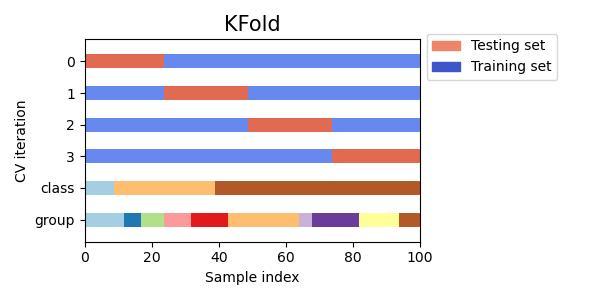
\includegraphics[width=.7\textwidth]{../figures/cv_kfold.png}
  \caption{A visualization of the splits of the data performed in cross validation. Here we see 4 $k$-folds which gives a total of 4 splits and iterations. \\
  \url{https://scikit-learn.org/stable/modules/cross_validation.html}}
  \label{fig:k_fold}
\end{figure}

\subsection{Study of $\lambda$ dependence for ridge and lasso regression}
To get the best possible predictions of our datasets we also implement lasso and ridge regression. These two methods are unlike OLS, dependent on a regularization parameter $\lambda$ where we have to compute which value that optimizes these two models. Similar to OLS we perform cross validation to find which degree of design matrix reduces the mean squared error of our predictions, only that we for ridge and lasso find the best $\lambda$ at the same time. This is because we for one degree would have one optimal $\lambda$ and for another degree have another. We therefore compute one cross validation for different values of $\lambda$ parameters for each degree. The degree and $\lambda$ giving the smallest MSE is then used for futher predictions

\subsection{Study of topography data}
After studying the franke function with added noise we look at real topography data from the mountains close to Stavanger in Norway. We perform the same analysis as we did with the Franke function except that we now assume that our data already contain some noise $\epsilon \sim N(0, \sigma^2)$ with an unknown standard deviation $\sigma$. We first standard scale our data by subtracting the mean and dividing by the standard deviation computed from the data:
\begin{align*}
  z_{scaled} = \frac{z-\bar{z}}{\hat{\sigma}_z}
\end{align*}
Our regression analysis will then be used to try to compute how the topography at the location actualy looks. Since the imported data includes  $3601 \times1801$ datapoints which would require more powerful hardware or atleast take a significant time to analyze, we choose an interesting location of indexes 100 to 141 in both directions and slice the data for every second index. That means we are left with input data of lower resoulution, but at the same time it enables us to do an analysis over a greater area.
\section{Results}
\subsection{Franke funtion}
\subsubsection{OLS scaling of data}
We first look if there is a need of scaling our data or not. As seen in figure \ref{fig:compare_scale} we have plotted the absoulute difference between the computed MSE and $R^2$ for different polynomial degrees. We see that the difference is so small especially for the
\ref{fig:r2_mse_5} we see them both plotted for design matrices up to a degree of 5 for $n=30$ steps and $\sigma=0.2$.
\begin{figure}[H]
  \begin{subfigure}{.5\textwidth}
    \centering
    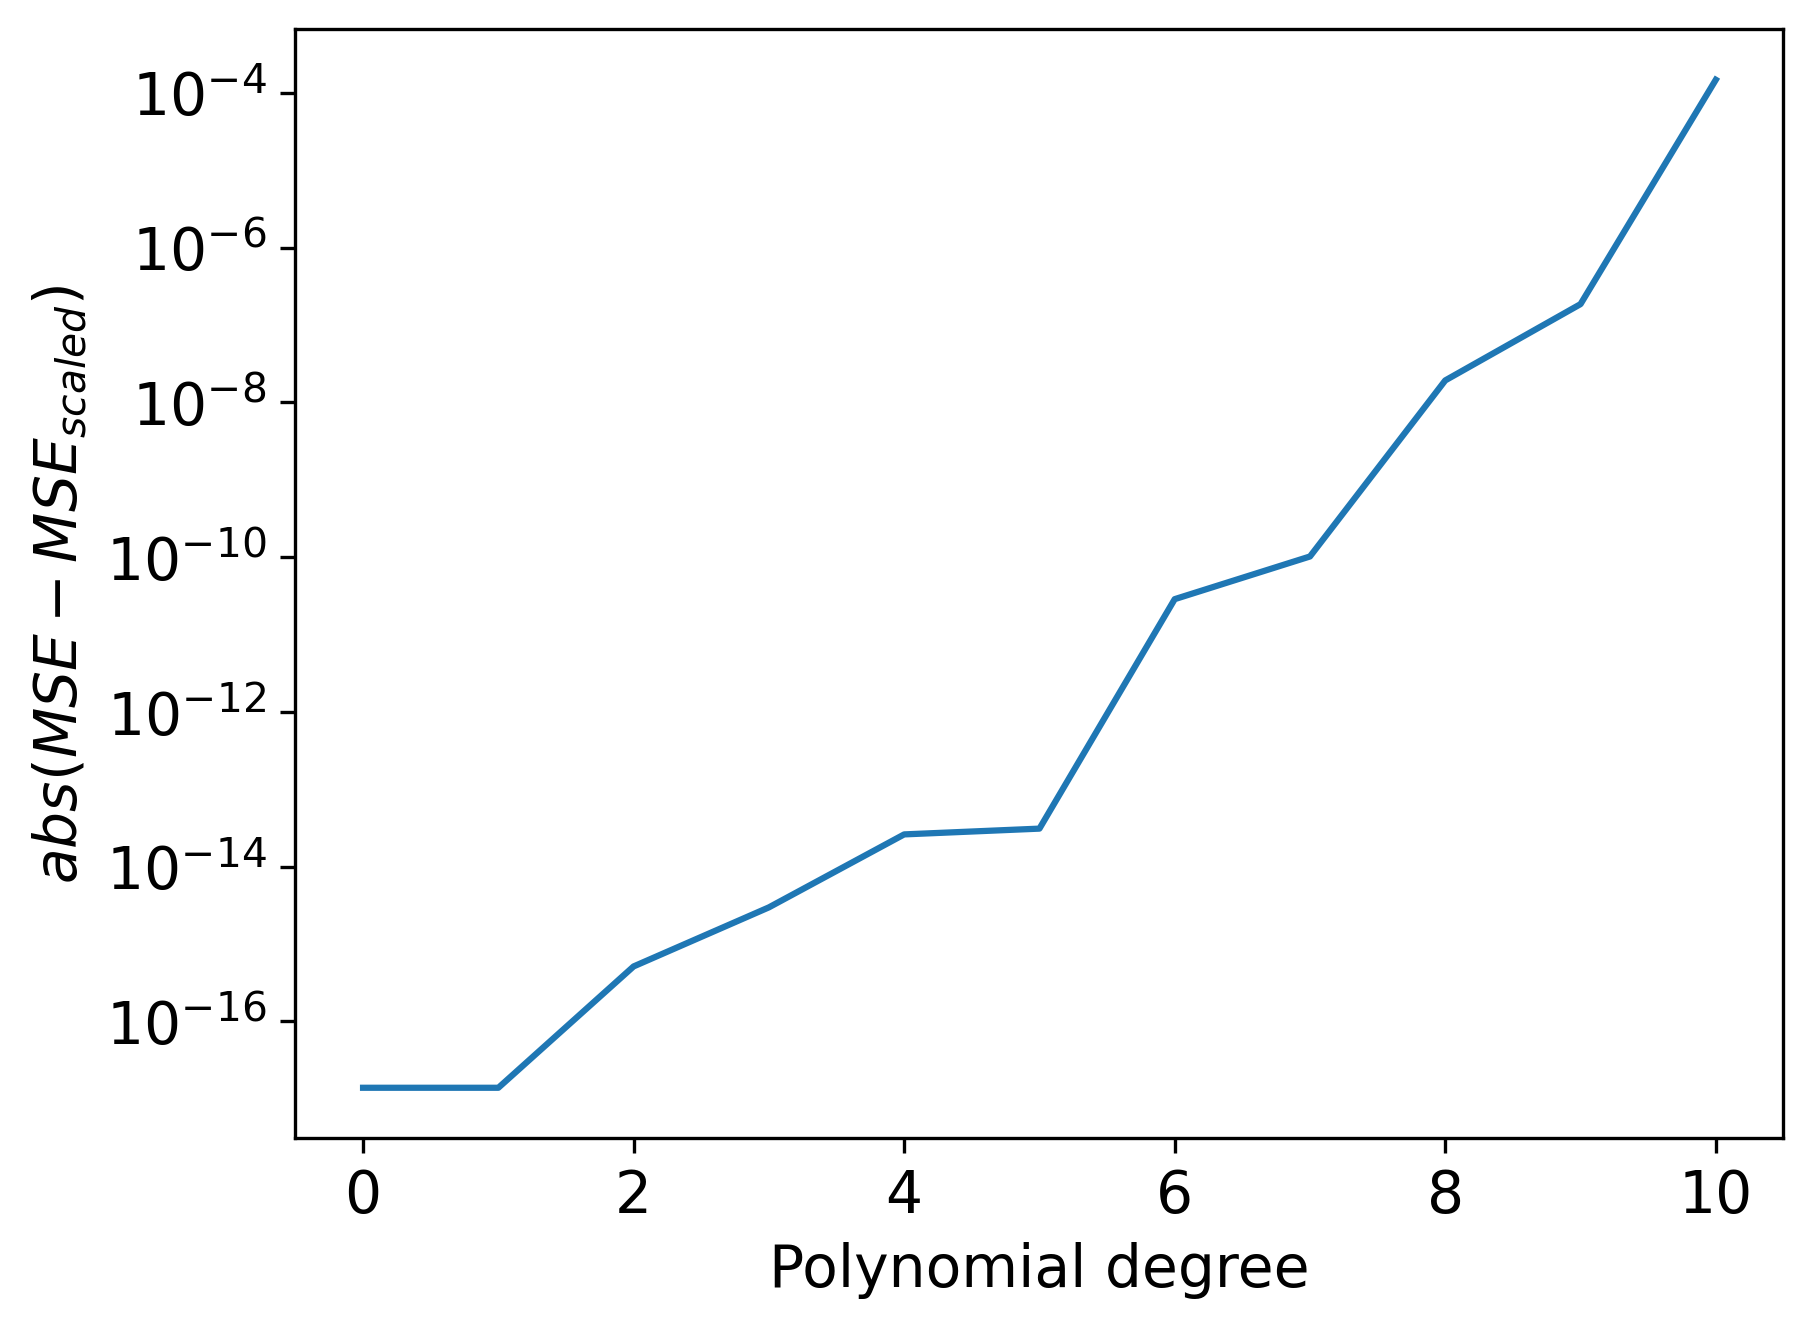
\includegraphics[width=\textwidth]{../figures/compare_scale_mse.png}
    \caption{$MSE$}
    \label{fig:}
  \end{subfigure}
  \begin{subfigure}{.5\textwidth}
    \centering
    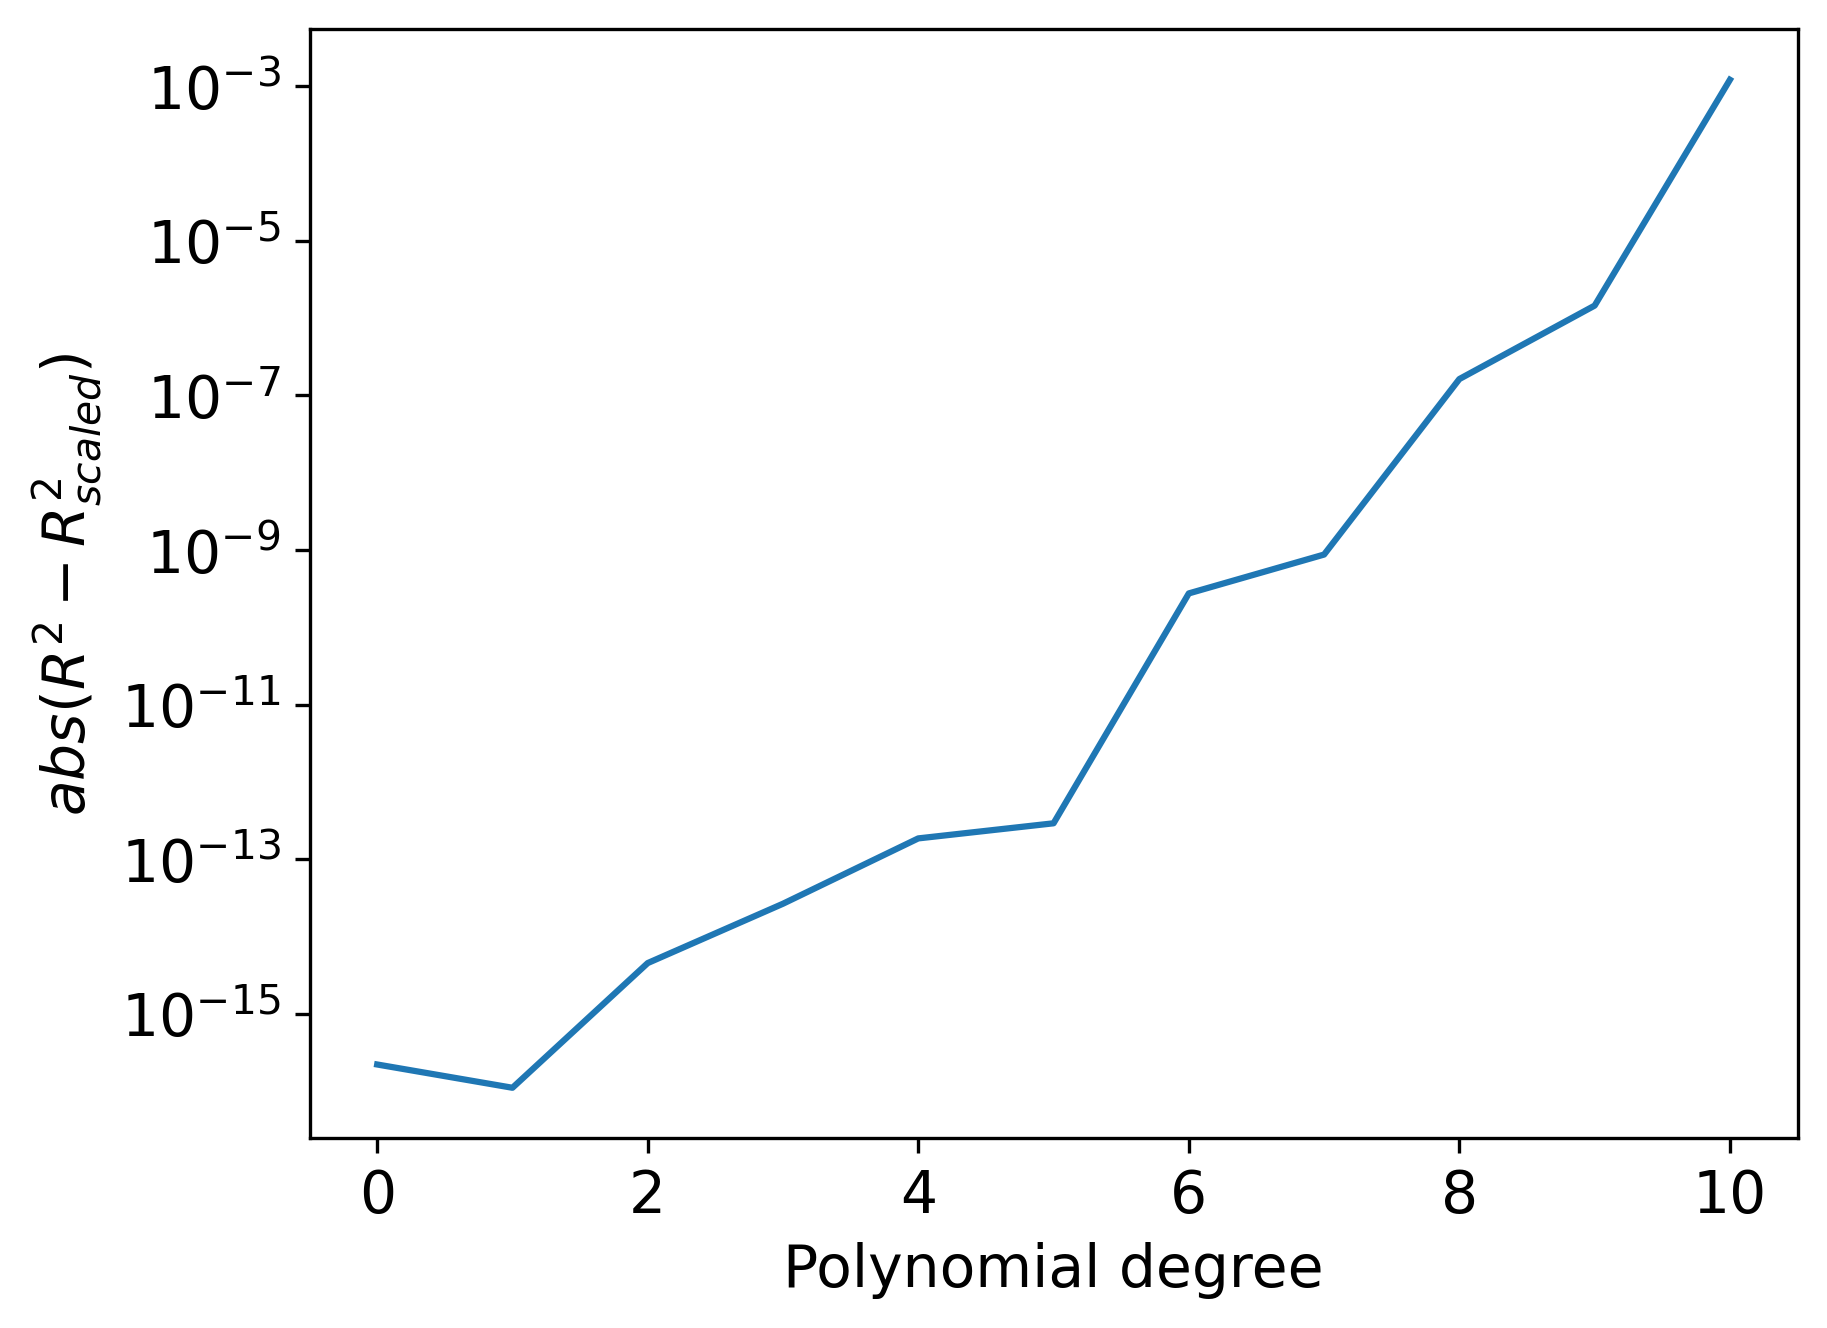
\includegraphics[width=\textwidth]{../figures/compare_scale_r2.png}
    \caption{$R^2$}
    \label{fig:}
  \end{subfigure}
  \caption{Comparison of MSE and $R^2$ between scaled and non-scaled data}
  \label{fig:compare_scale}
\end{figure}
We see that the difference between the scaled and non-scaled data are so small especially for lower polynomial degrees which indicate that scaling of our data is unnecesary.

\subsubsection{OLS MSE and $R^2$}

We continue with our non-scaled data and look at how the mean square error and R squared behave for design matrices of different degrees. Underneeth in figure \ref{fig:r2_mse_5} we see them both plotted for design matrices up to a degree of 5 for $n=30$ steps and $\sigma=0.2$.
\begin{figure}[H]
  \begin{subfigure}{.5\textwidth}
    \centering
    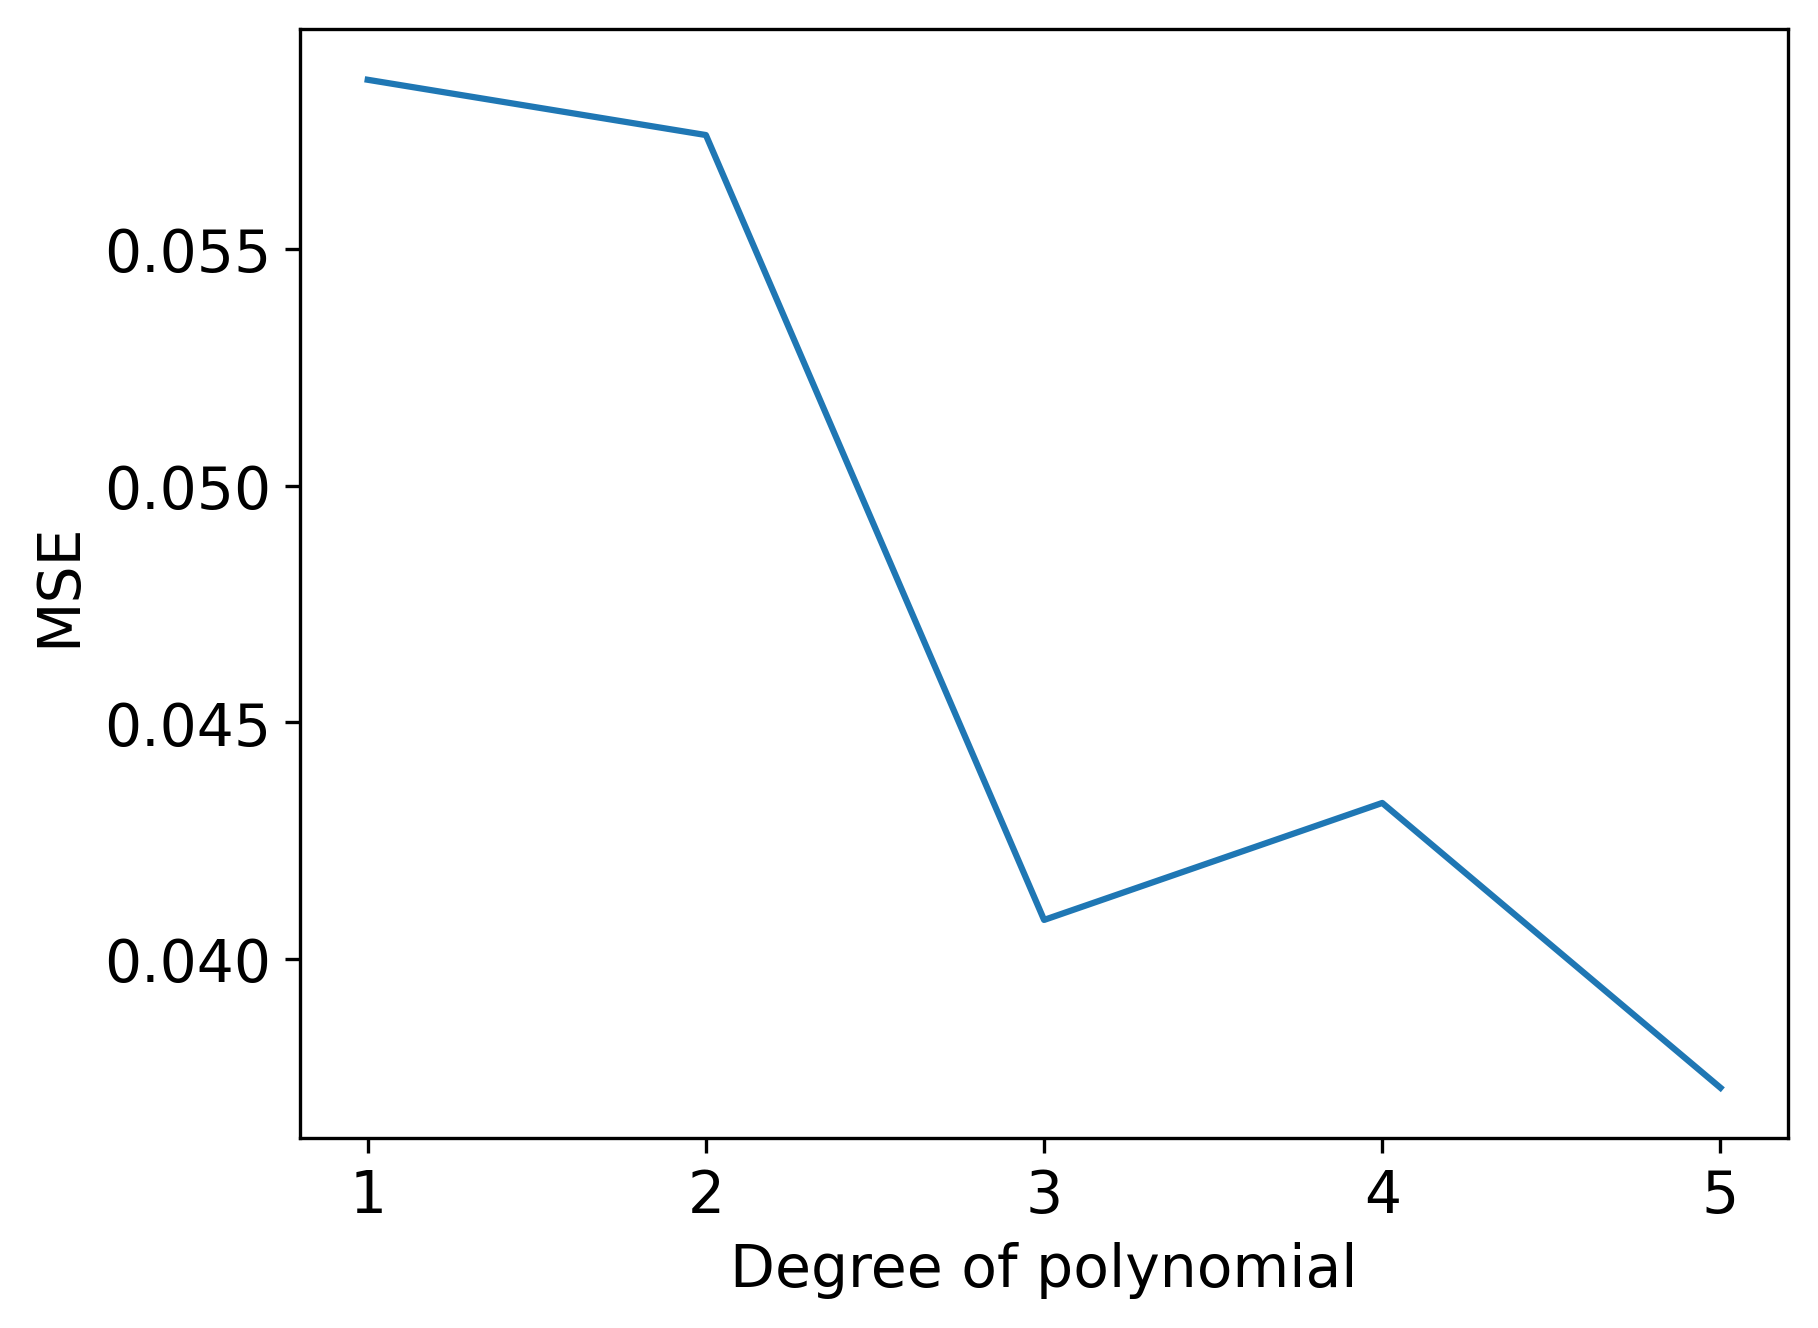
\includegraphics[width=\textwidth]{../figures/mse_ols_5.png}
    \caption{$MSE$}
    \label{fig:}
  \end{subfigure}
  \begin{subfigure}{.5\textwidth}
    \centering
    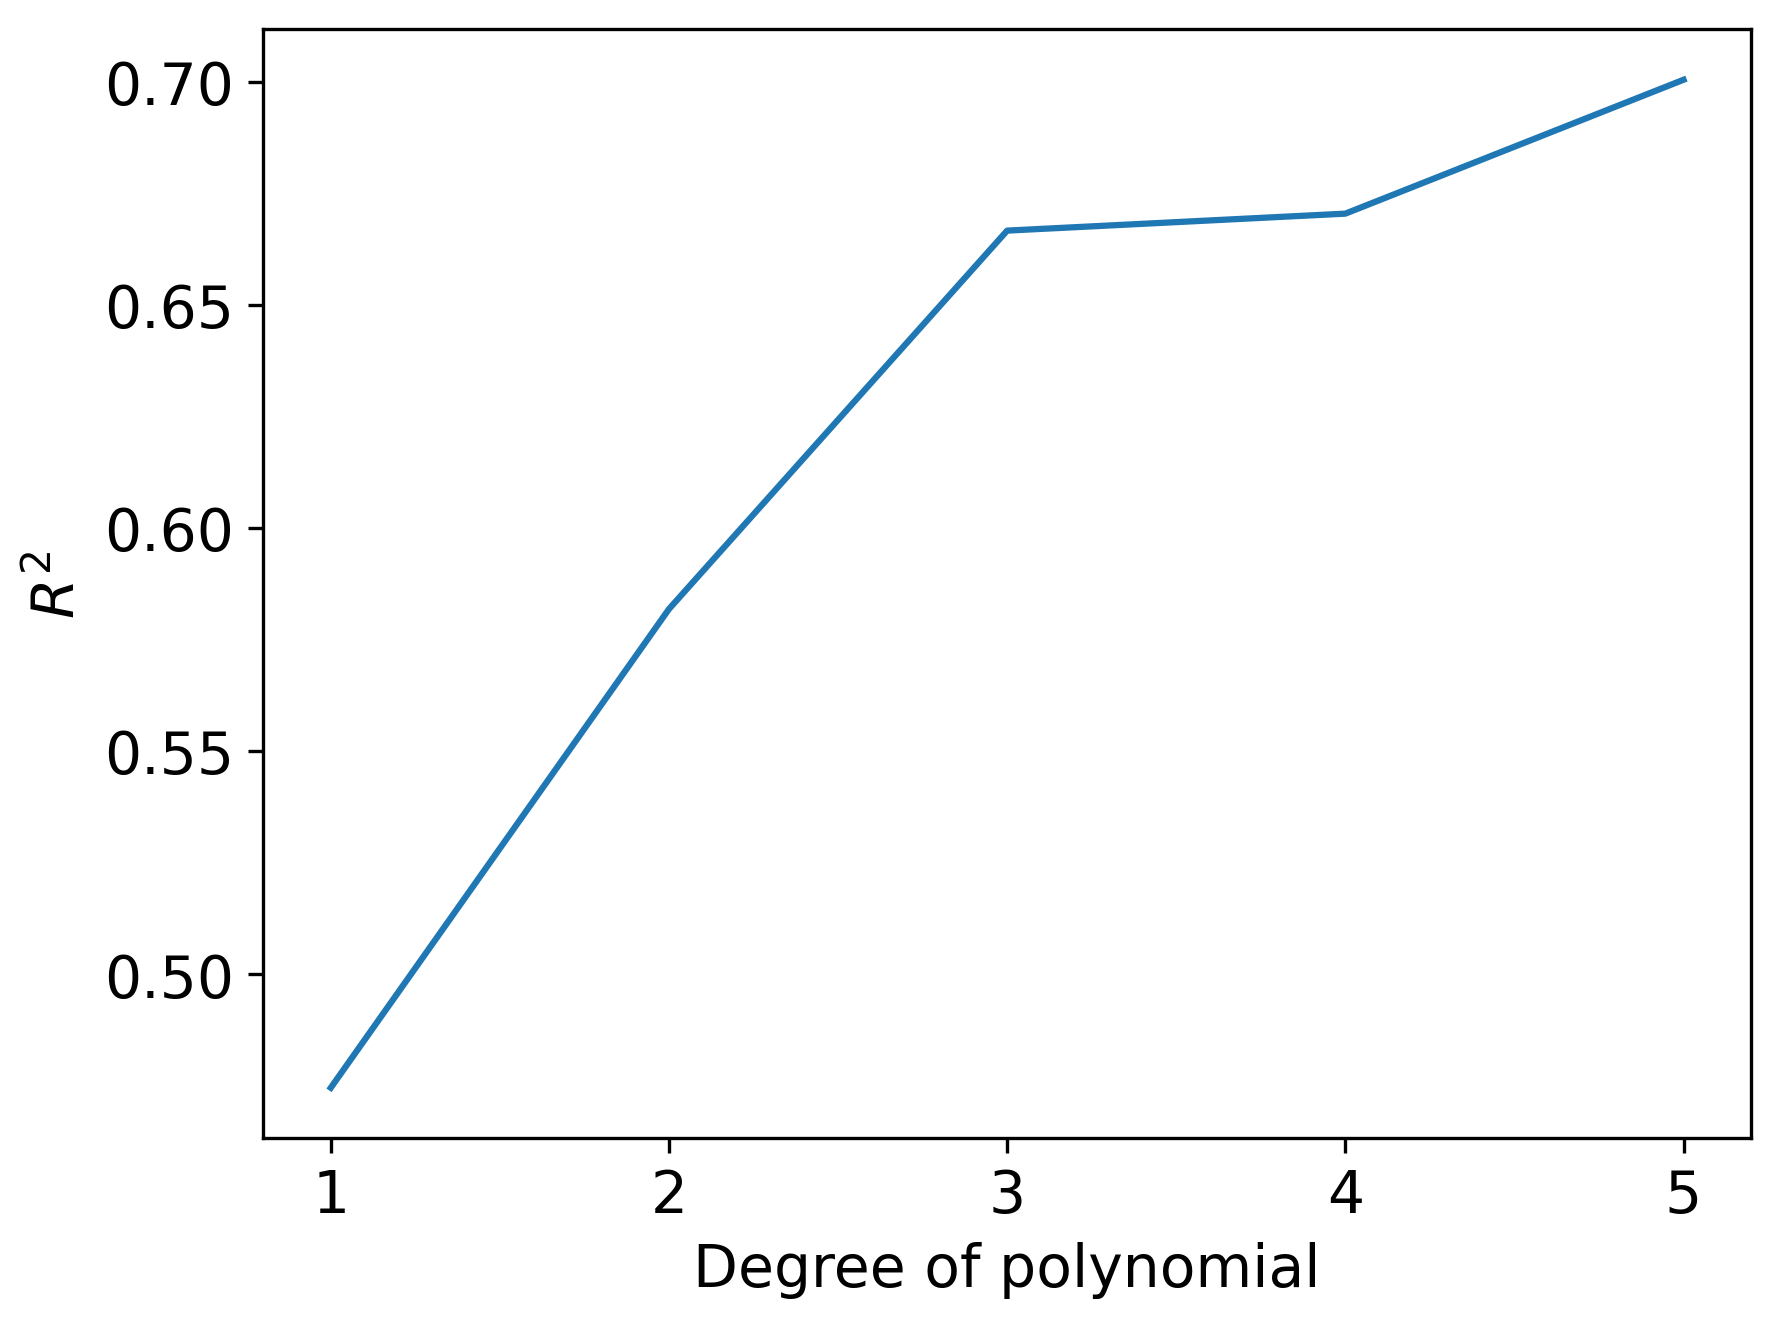
\includegraphics[width=\textwidth]{../figures/r2_ols_5.png}
    \caption{$R^2$}
    \label{fig:}
  \end{subfigure}
  \caption{plots of MSE and $R^2$ for the franke function for an error $\epsilon \sim N(0, \sigma^2)$ with $\sigma=0.2$ and 31 points in each direction}
  \label{fig:r2_mse_5}
\end{figure}
Above in figure \ref{fig:r2_mse_5} we see a clear reduction in MSE for an increase in polynomial degree of the design matrix. For $R^2$ we see increasing values for higher degrees, with degree 5 giving us the lowest MSE and highest $R^2$ indicating degree 5 being the most optimal degree.

We continue to look into MSE and $R^2$ but now comparing the use of train or test data in the prediction of $z$. We continue using $n=30$ steps and $\sigma=0.2$. In figure \ref{fig:train_test} we see a single run and the following MSE and $R^2$ while we in figure \ref{fig:train_test_resample} see a plot of a resample of the noise data giving us 100 unique datasets to take the mean of.
\begin{figure}[H]
  \begin{subfigure}{.5\textwidth}
    \centering
    \includegraphics[width=\textwidth]{../figures/mse_train_test.png}
    \caption{$MSE$}
    \label{fig:}
  \end{subfigure}
  \begin{subfigure}{.5\textwidth}
    \centering
    \includegraphics[width=\textwidth]{../figures/r2_train_test.png}
    \caption{$R^2$}
    \label{fig:}
  \end{subfigure}
  \caption{MSE and $R^2$ computed from both the train and test sample}
  \label{fig:train_test}
\end{figure}
Above we see that both the MSE and $R^2$ from the test sample seem to start deviating from the train sample at degrees higher than 5 which indicates overfitting for greater degrees.
\begin{figure}[H]
  \begin{subfigure}{.5\textwidth}
    \centering
    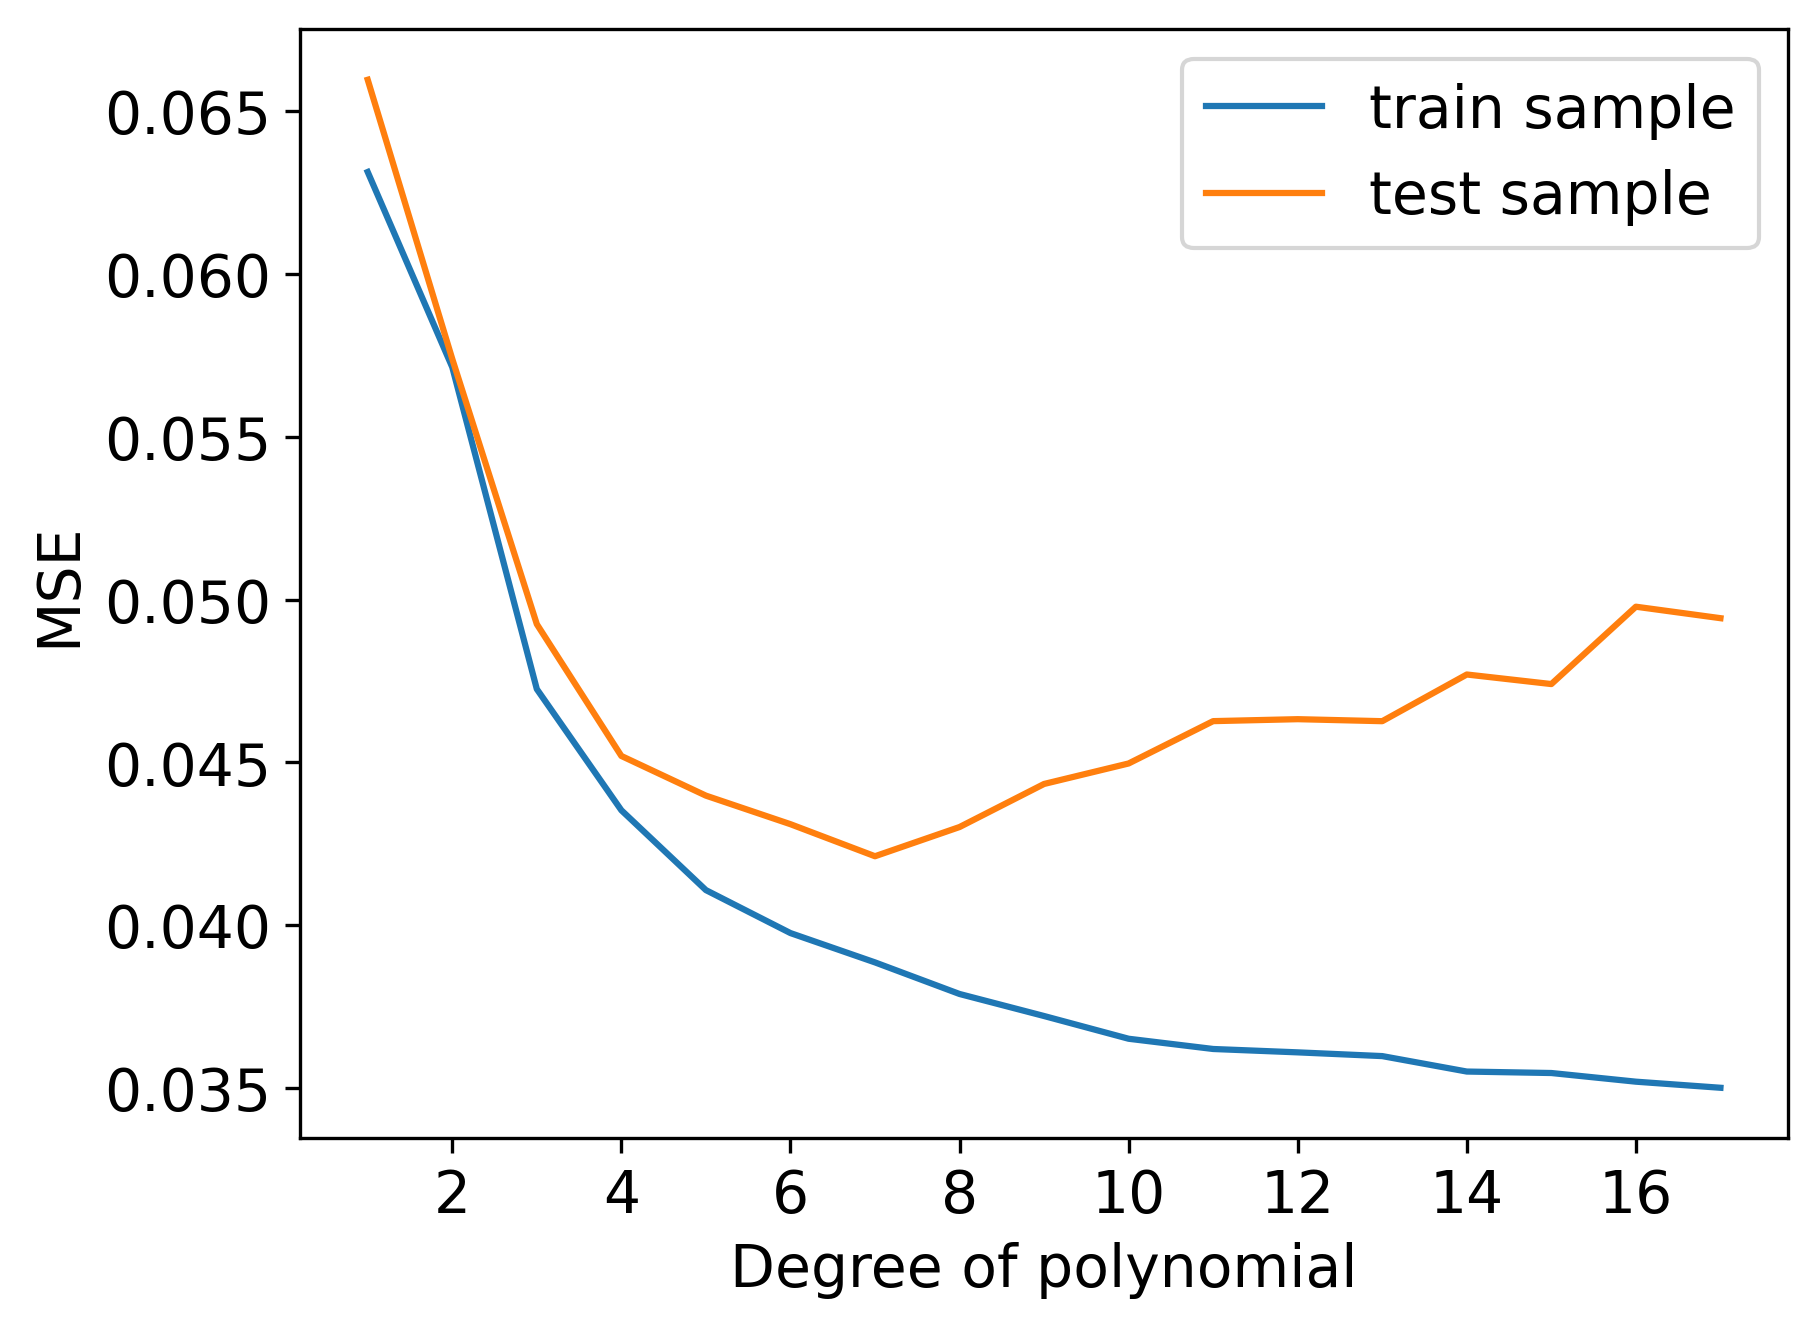
\includegraphics[width=\textwidth]{../figures/MSE_train_test_resample.png}
    \caption{$MSE$}
    \label{fig:train_test_resample_mse}
  \end{subfigure}
  \begin{subfigure}{.5\textwidth}
    \centering
    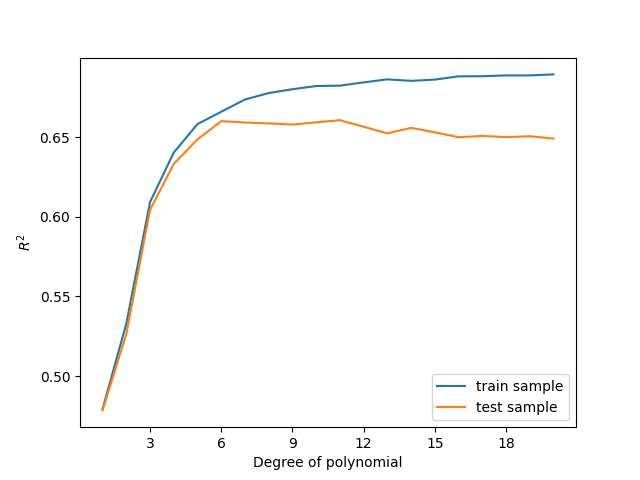
\includegraphics[width=\textwidth]{../figures/R2_train_test_resample.png}
    \caption{$R^2$}
    \label{fig:}
  \end{subfigure}
  \caption{An average of MSE and $R^2$ computed from both the train and test sample over 100 unique samples}
  \label{fig:train_test_resample}
\end{figure}
Above in figure \ref{fig:train_test_resample} we get a smoother plot showing the smallest MSE obtained from a degree of 6 indicating this being the best polynomial degree for OLS regression of the franke function. The $R^2$ show the same tendency but looks like having the greatest values at a degree of 8.

\subsubsection{OLS variation of $\beta$ paramers}

To see how the $\beta$ parameters variate from different choices of degrees we plot them for a degree up to 5 indicated in figure \ref{fig:beta} below:
\begin{figure}[H]
  \centering
  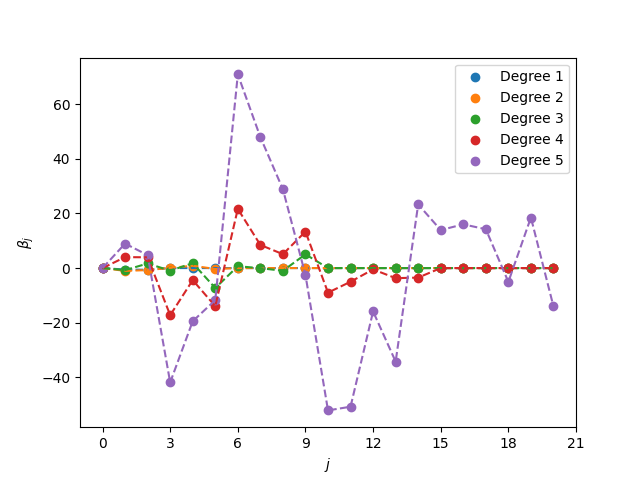
\includegraphics[width=.7\textwidth]{../figures/beta_degree.png}
  \caption{}
  \label{fig:beta}
\end{figure}
We see an increase in distance between the $\beta$ parameteres for an increasing polynomial degree. When we at the same time look at table \ref{tab:beta} we see that the parameters for a degree of 5 come with great variance. This is especially true for parameters of index in the interval [6,14] which we also see in figure \ref{fig:beta} have larger values than the rest. This may be an indication of overfitting, but looking back at our resampled train test MSE plot in figure \ref{fig:train_test_resample_mse} we see that we for a degree of 5 have lower MSE than larger polynomial degrees.

\begin{table}[H]
  \caption{Variance of the $\beta$ parameters for test and train data for a design matrix of polynomial degree 5. Calculated by $Var(\boldsymbol{\beta}) = diag(\sigma^2(X^T X)^{-1}$)}
  \label{tab:beta}
  \centering
  \begin{tabular}{|c|c|c|}
    \hline
    $\boldsymbol{\beta}$ &\textbf{Test data} & \textbf{Train data} \\\hline
    $\beta_{0}$ & 0.04 & 0.01 \\
    $\beta_{1}$ & 5.22 & 1.31 \\
    $\beta_{2}$ & 6.00 & 1.27 \\
    $\beta_{3}$ & 139.88 & 31.56 \\
    $\beta_{4}$ & 90.01 & 19.04 \\
    $\beta_{5}$ & 149.50 & 31.37 \\
    $\beta_{6}$ & 723.58 & 162.55 \\
    $\beta_{7}$ & 364.34 & 90.68 \\
    $\beta_{8}$ & 555.61 & 83.97 \\
    $\beta_{9}$ & 787.29 & 163.88 \\
    $\beta_{10}$ & 794.84 & 179.33 \\
    $\beta_{11}$ & 521.51 & 104.67 \\
    $\beta_{12}$ & 424.30 & 88.62 \\
    $\beta_{13}$ & 625.04 & 98.00 \\
    $\beta_{14}$ & 880.18 & 180.91 \\
    $\beta_{15}$ & 122.43 & 27.74 \\
    $\beta_{16}$ & 102.30 & 20.80 \\
    $\beta_{17}$ & 80.15 & 19.80 \\
    $\beta_{18}$ & 108.00 & 19.14 \\
    $\beta_{19}$ & 105.44 & 20.14 \\
    $\beta_{20}$ & 134.90 & 27.84 \\
    \hline
  \end{tabular}
\end{table}

\subsubsection{OLS bias variance tradeoff}

To futher analyze our models dependence on polynomial degree we have a plot of the bias variance tradeoff in figure \ref{fig:bias_variance} for a degree up to 15 using $n=22$ steps and a noise standard deviation of $\sigma=0.2$.
\begin{figure}[H]
  \centering
  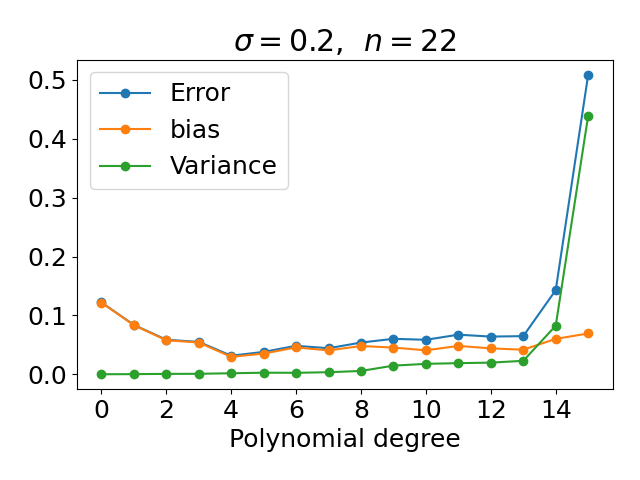
\includegraphics[width=.7\textwidth]{../figures/bias_variance_tradeoff.png}
  \caption{The bias variance tradeoff for the Franke function using 100 bootstrap iteration together with $n=22$ steps and a noise standard deviation of $\sigma=0.2$}
  \label{fig:bias_variance}
\end{figure}
We se above in figure \ref{fig:bias_variance} areas of both high variance and low bias and low variance and relative high bias. We also see that the area of lowest MSE for a degree of 6 is where both the bias and variance together is at their lowest. A futher increase in polynomial degree gives mostly a variance dominated error contribution while we at lower polynomial degrees see that the bias is what contributes the most to the error. When we look at figure \ref{fig:bias_variance_100} we see another trend especially for higher polynomial degrees. Here the variance stays low which may together with the low mse indicate that we dont as easy overfit our data when we have more of it at hand.
\begin{figure}[H]
  \centering
  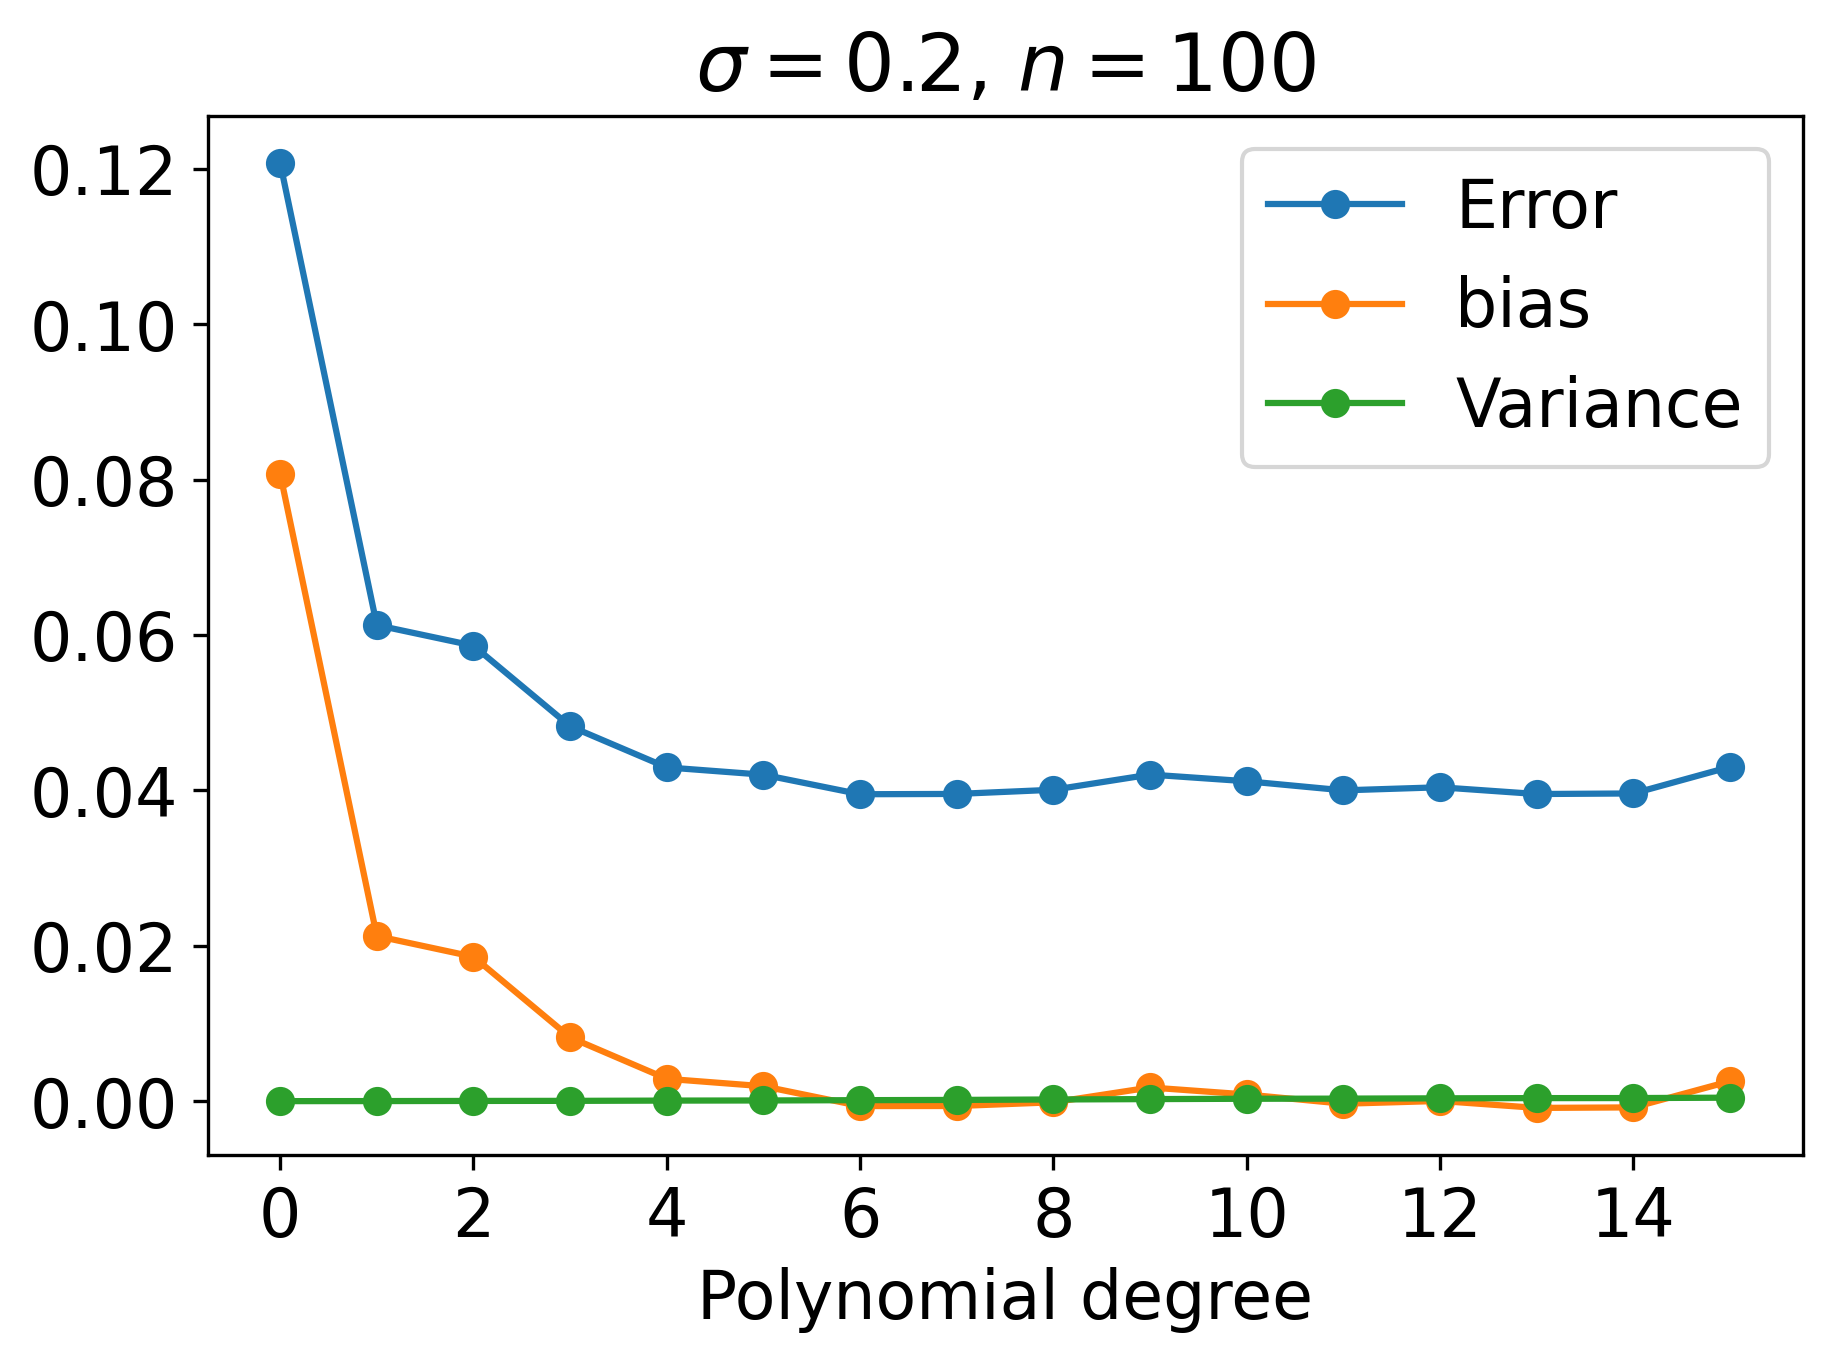
\includegraphics[width=.7\textwidth]{../figures/bias_variance_100.png}
  \caption{The bias variance tradeoff for the Franke function using 100 bootstrap iteration together with $n=100$ steps and a noise standard deviation of $\sigma=0.2$}
  \label{fig:bias_variance_100}
\end{figure}
\subsubsection{OLS cross validation}
From the implementation of cross validation we get the following comparison plot in figure \ref{fig:cv_comp} for data with $n=30$ steps and $\sigma=0.2$ for 100 bootstrap iterations compared to cross validation of both 5 and 10 $k$-folds:
\begin{figure}[H]
  \begin{subfigure}{.5\textwidth}
    \centering
    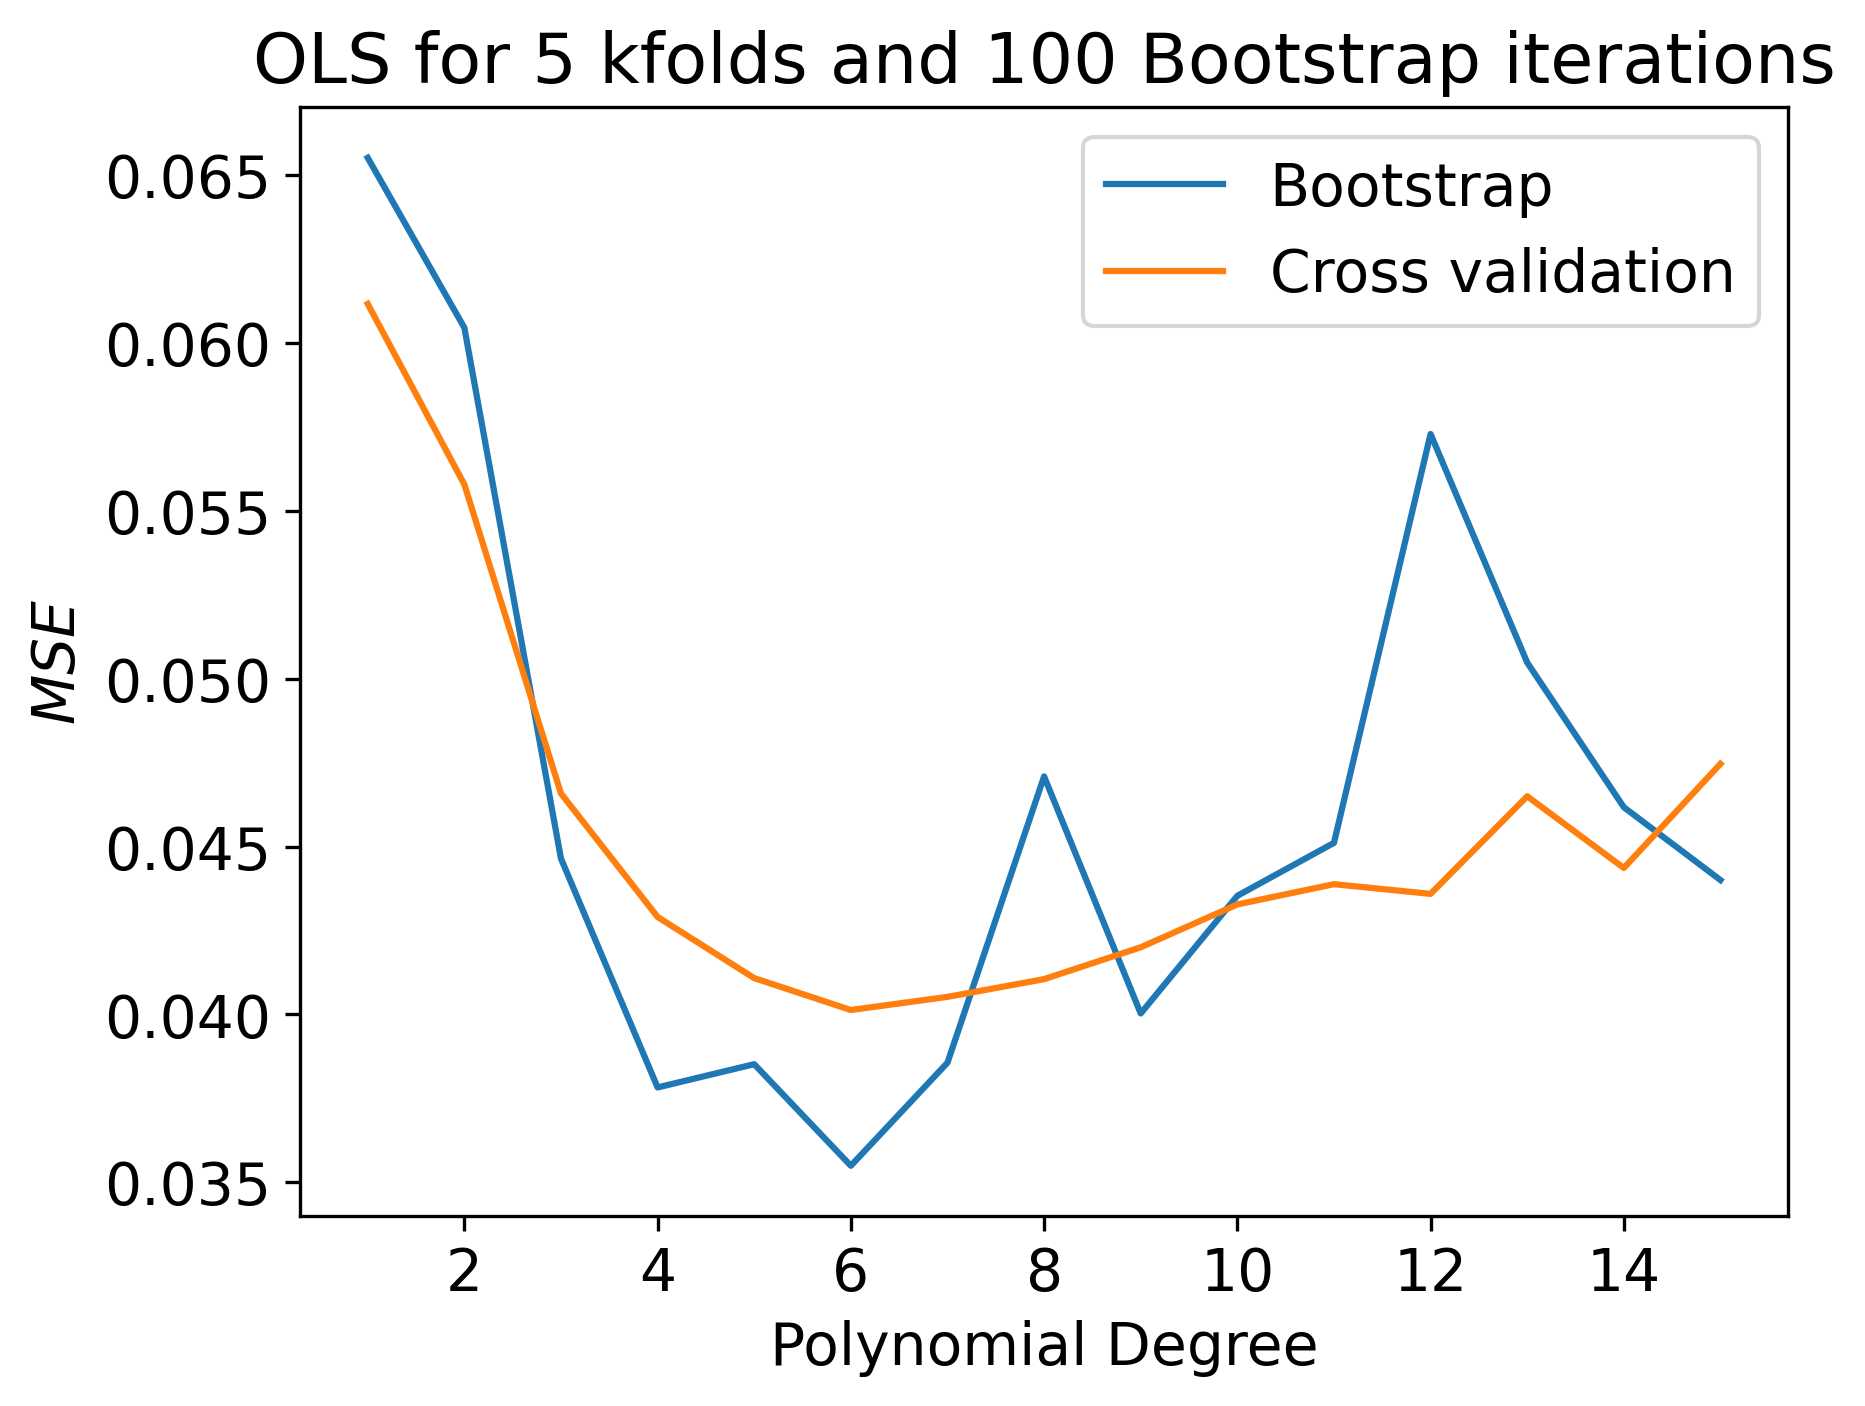
\includegraphics[width=\textwidth]{../figures/boot_cv_comp_OLS_100_5.png}
    \caption{5 $k$-folds}
    \label{fig:train_test_resample_mse}
  \end{subfigure}
  \begin{subfigure}{.5\textwidth}
    \centering
    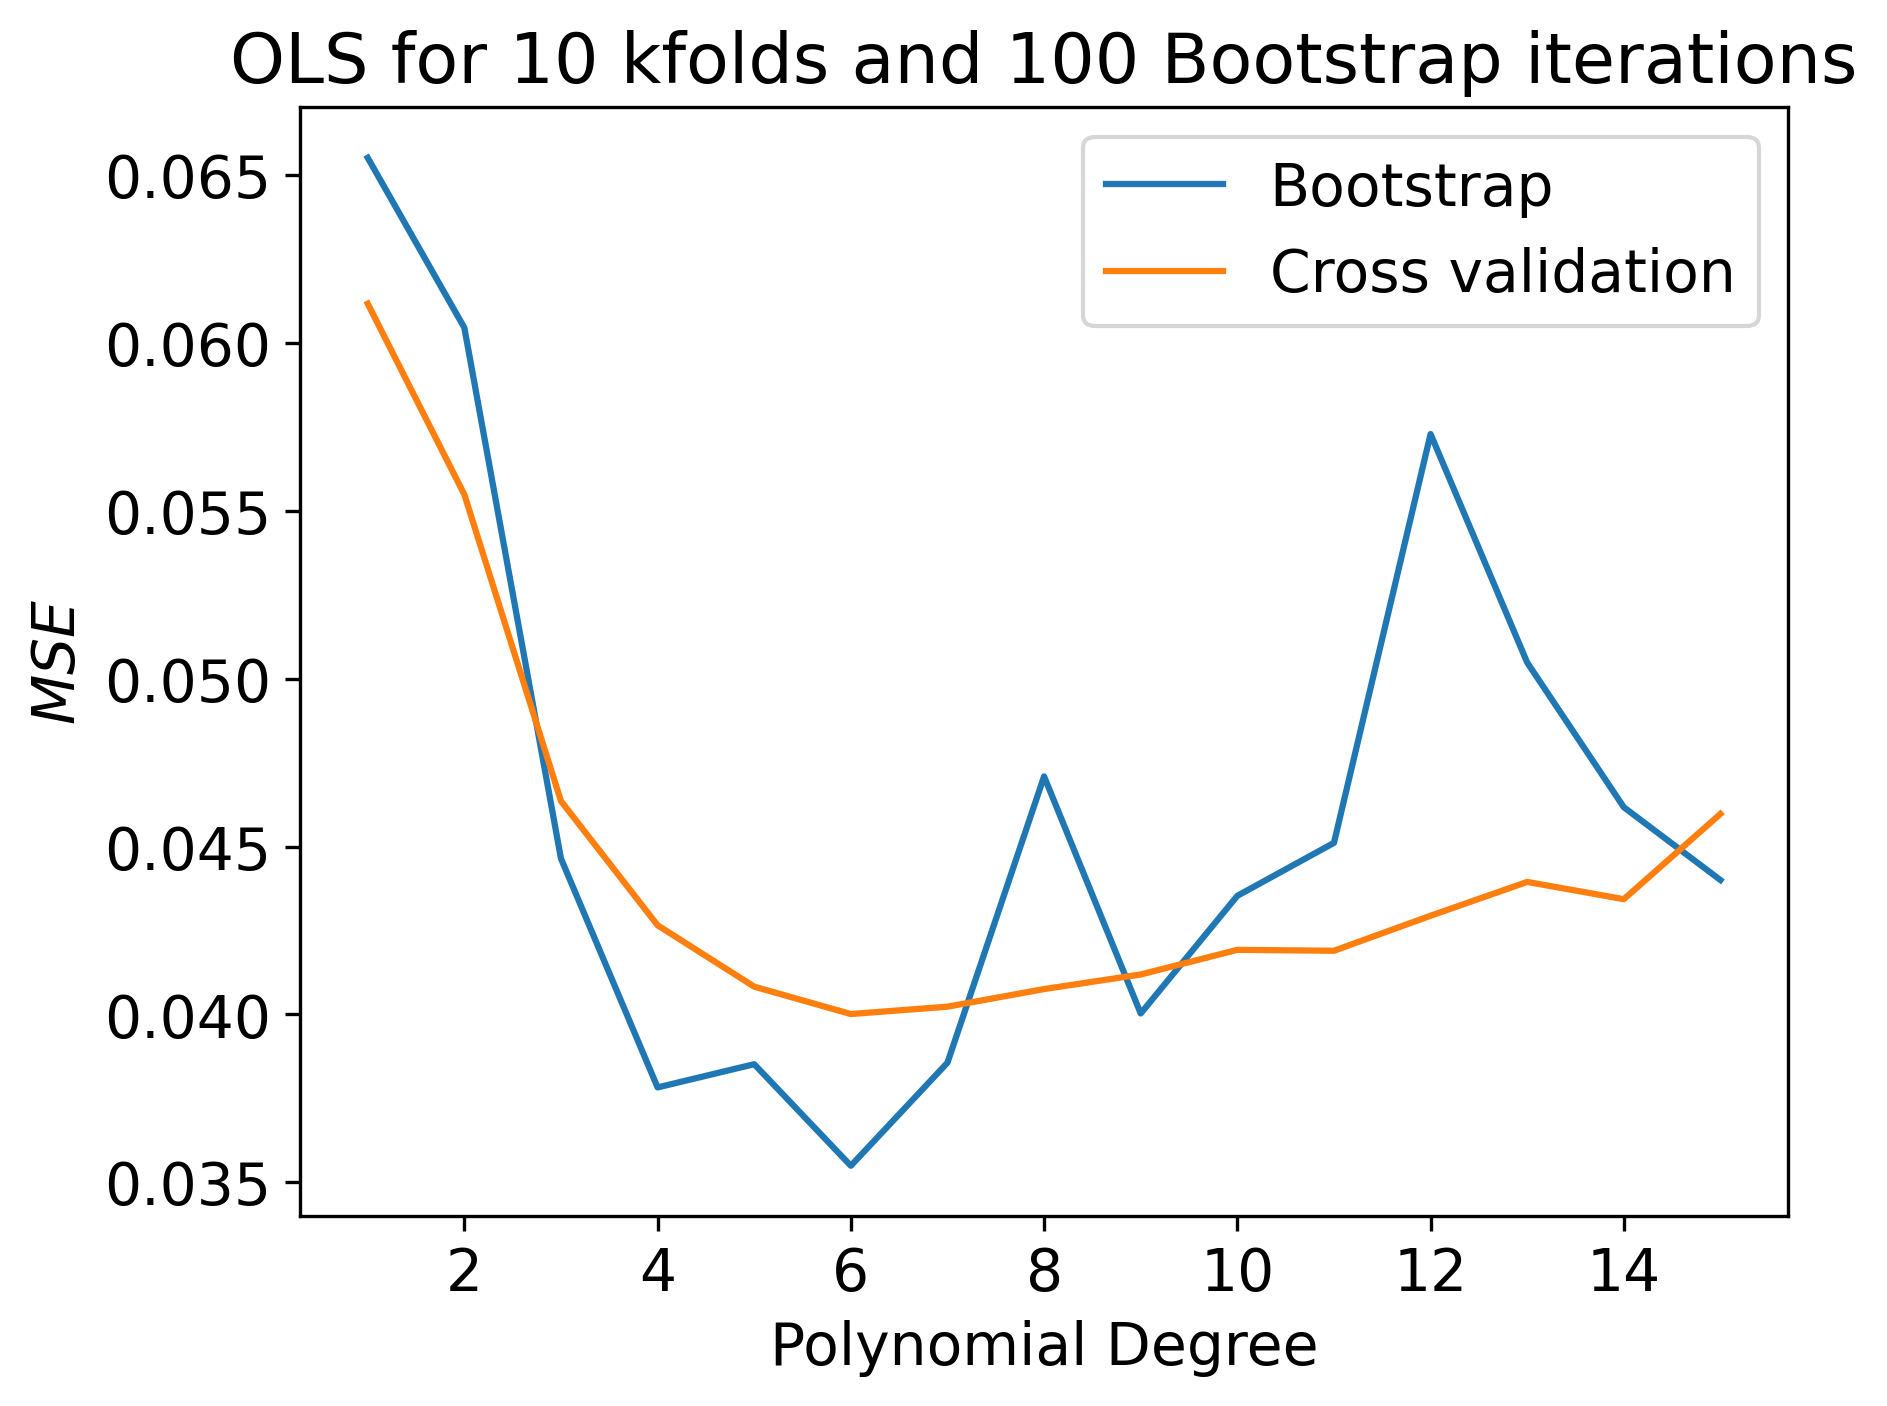
\includegraphics[width=\textwidth]{../figures/boot_cv_comp_OLS_100_10.png}
    \caption{10 $k$-folds}
    \label{fig:}
  \end{subfigure}
  \caption{A comparison between bootstrap and cross validation for datasets with $n=30$ steps, noise standard deviation $\sigma=0.2$ and 100 bootstrap iterations}
  \label{fig:cv_comp}
\end{figure}
We see different results for bootstrap and cross validation for both 5 and 10 $k$-folds. The difference between the $k$-folds are quite small, but the difference from the bootstrap is for some polynomial degrees higher than others. Underneeth in figure \ref{fig:cv_comp_01} we see a comparison for the same amount of data only with an error standard deviation of $\sigma=0.1$ instead of 0.2:
\begin{figure}[H]
  \centering
  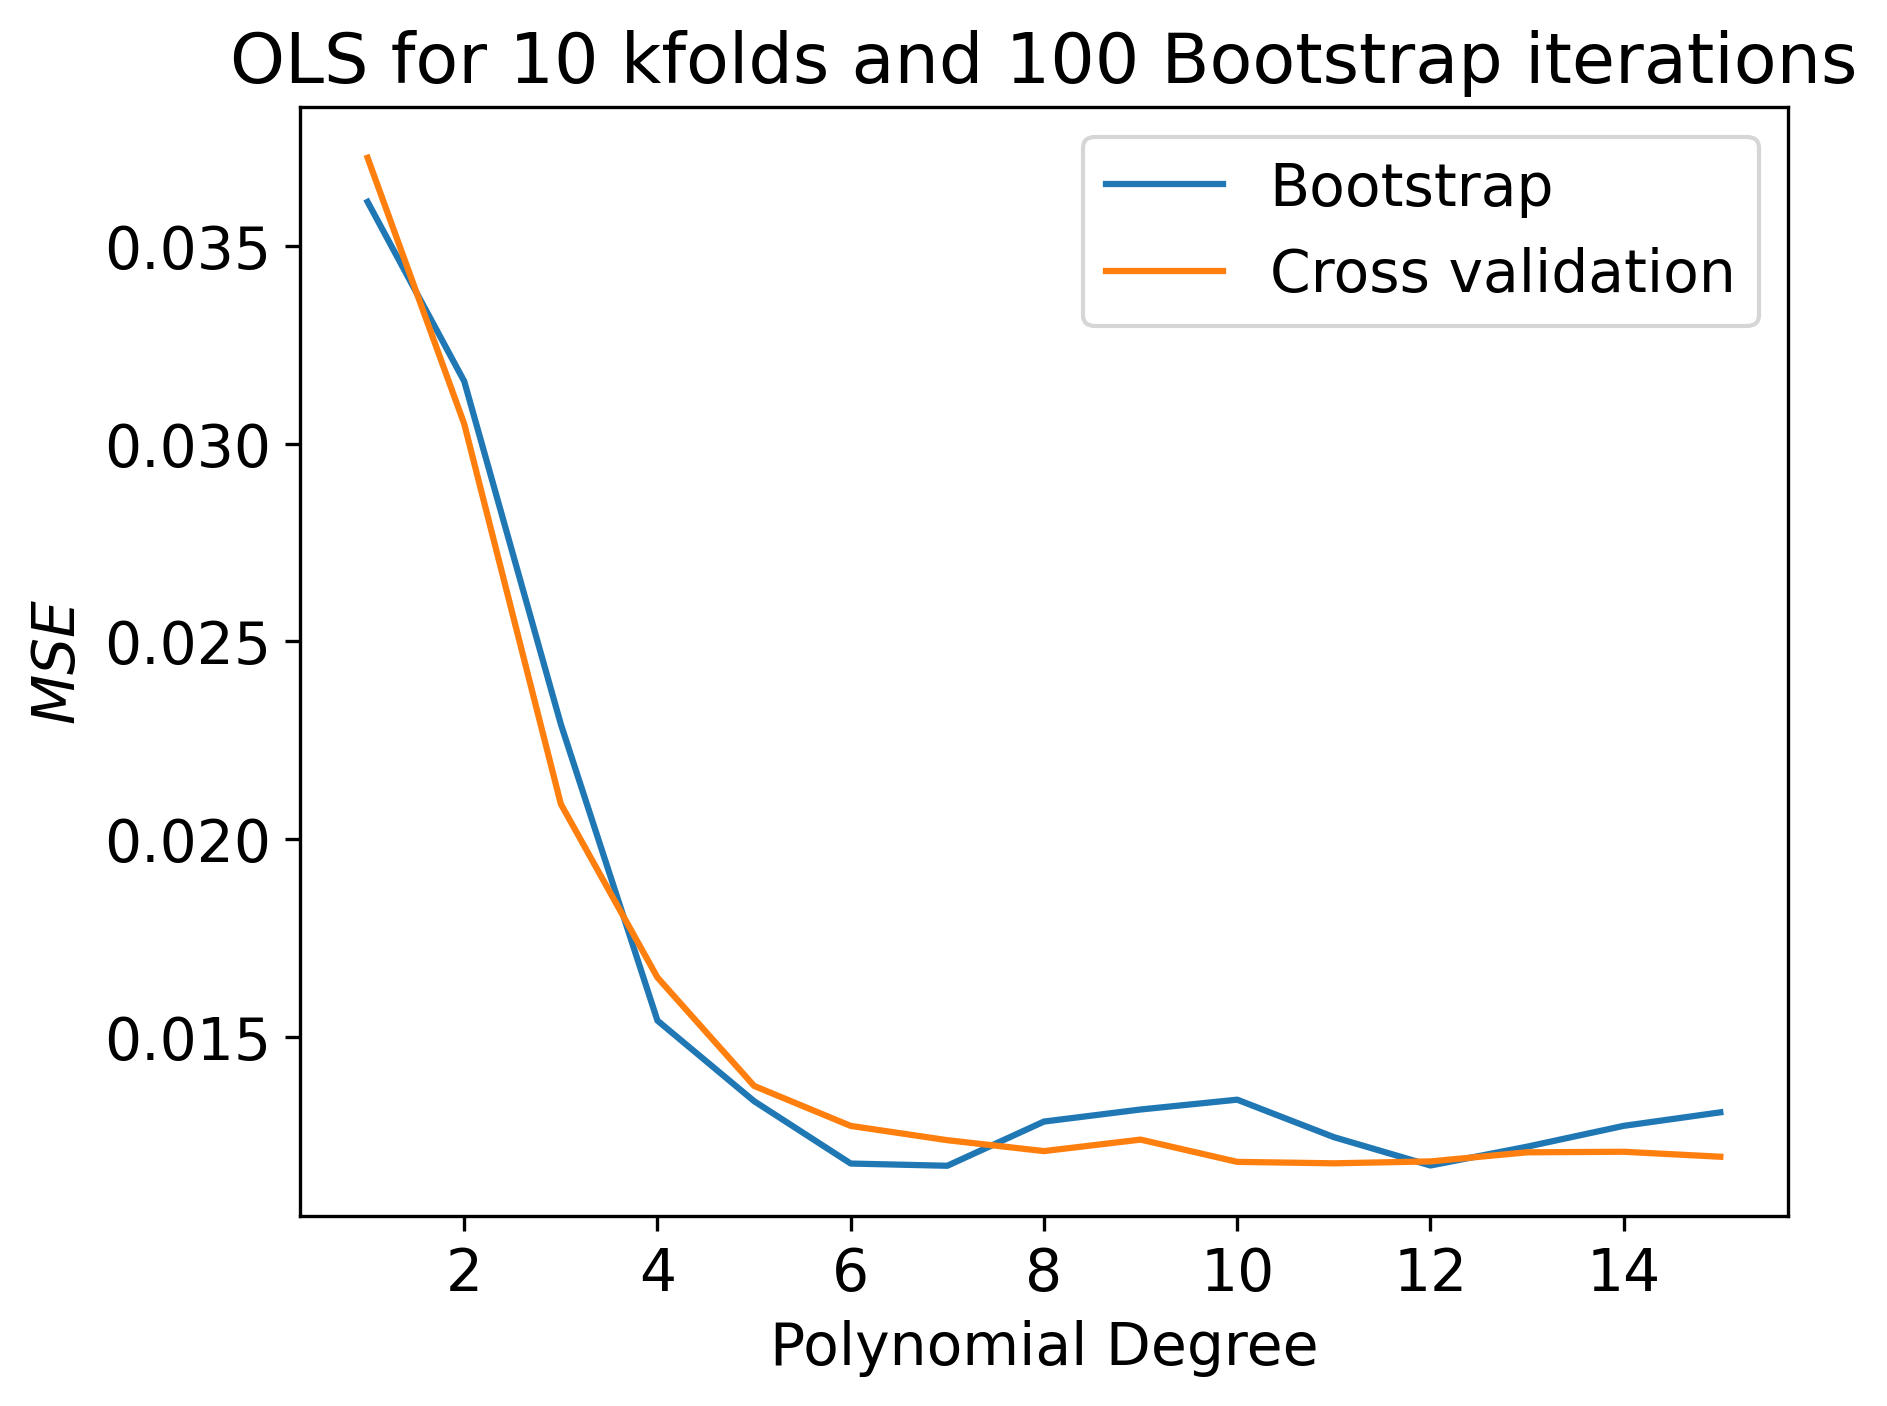
\includegraphics[width=.7\textwidth]{../figures/boot_cv_comp_01.png}
  \caption{A comparison between bootstrap and cross validation for datasets with $n=30$ steps, noise standard deviation $\sigma=0.1$ and 100 bootstrap iterations}
  \label{fig:cv_comp_01}
\end{figure}
We see above in figure \ref{fig:cv_comp_01} that the bootstrap gives more similar results to the cross validation method for a lower noise standard deviation. At the same time we see the same trend for the bootstrap with lower MSE values around a degree of 6 and 12 while it still gives higher MSE for around a degree of 10 and above 13.

We continue using the cross validation method to compute for which degree we get the lowest mean squared errors. As we see under in figure \ref{fig:best_OLS}
\begin{figure}[H]
  \centering
  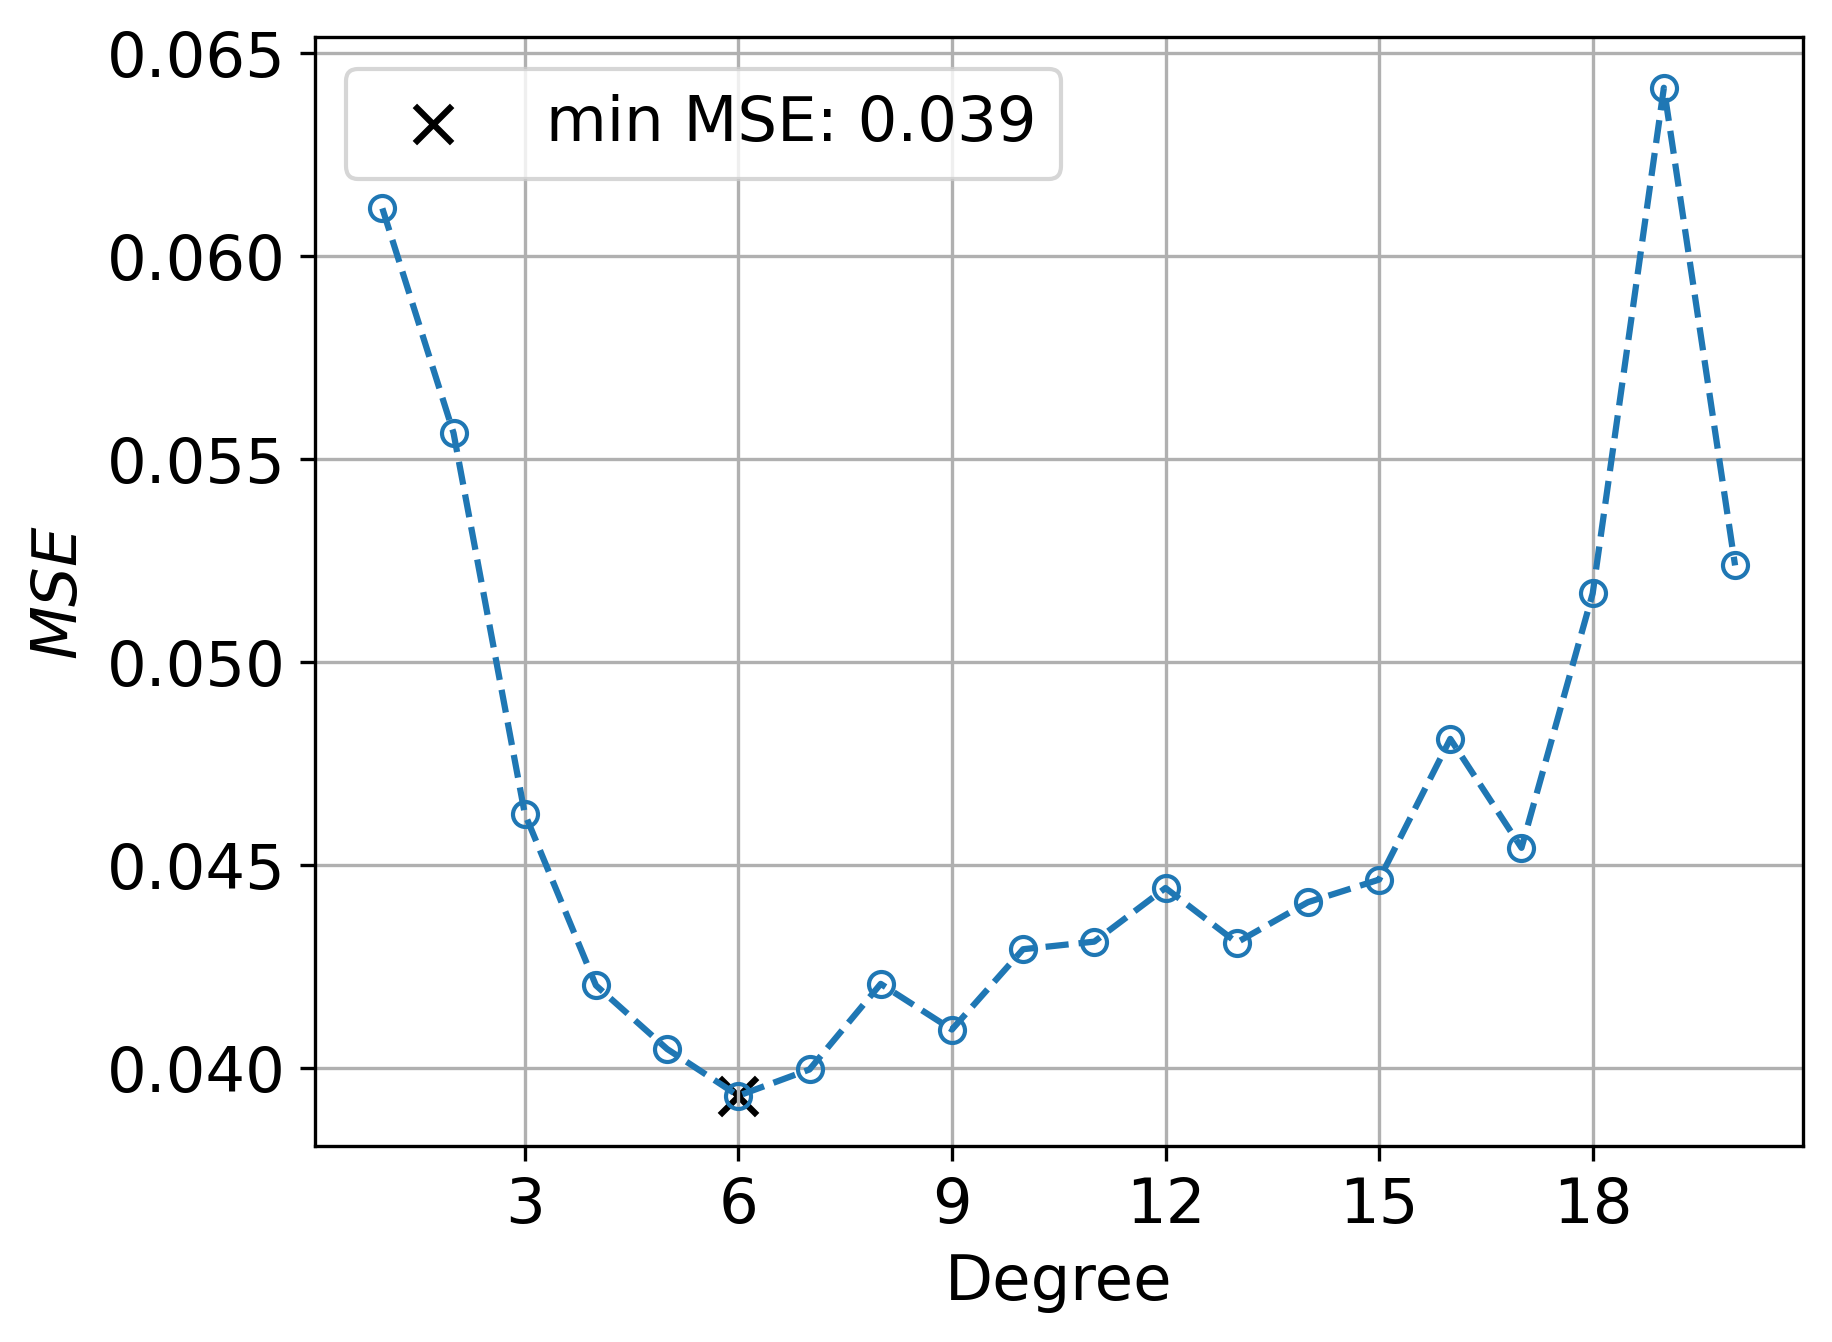
\includegraphics[width=.7\textwidth]{../figures/best_lambda_OLS_02_franke.png}
  \caption{Cross validation to find which polynomial degree gives the lowest MSE for data with $n=30$ steps and noise standard deviation $\sigma=0.2$}
  \label{fig:best_OLS}
\end{figure}

Above in figure \ref{fig:best_OLS} we see similar to figure \ref{fig:cv_comp} That we for a degree of 6 minimize the MSE for OLS regression. This means that if we want to compute the best possible prediction $\tilde{z}$ we should use a design matrix of degree 6.

\subsubsection{Ridge and Lasso bias variance tradeoff}
In the same way as for ordinary least squares we look at the bias variance tradeoff, only that we now have another parameter $\lambda$ that influences the tradeoff. Under in figure \ref{fig:ridge_tradeoff} and figure \ref{fig:lasso_tradeoff} we see the tradeoff for different choices of $\lambda$ for both Ridge and Lasso regression
\begin{figure}[H]
  \begin{subfigure}{.5\textwidth}
    \centering
    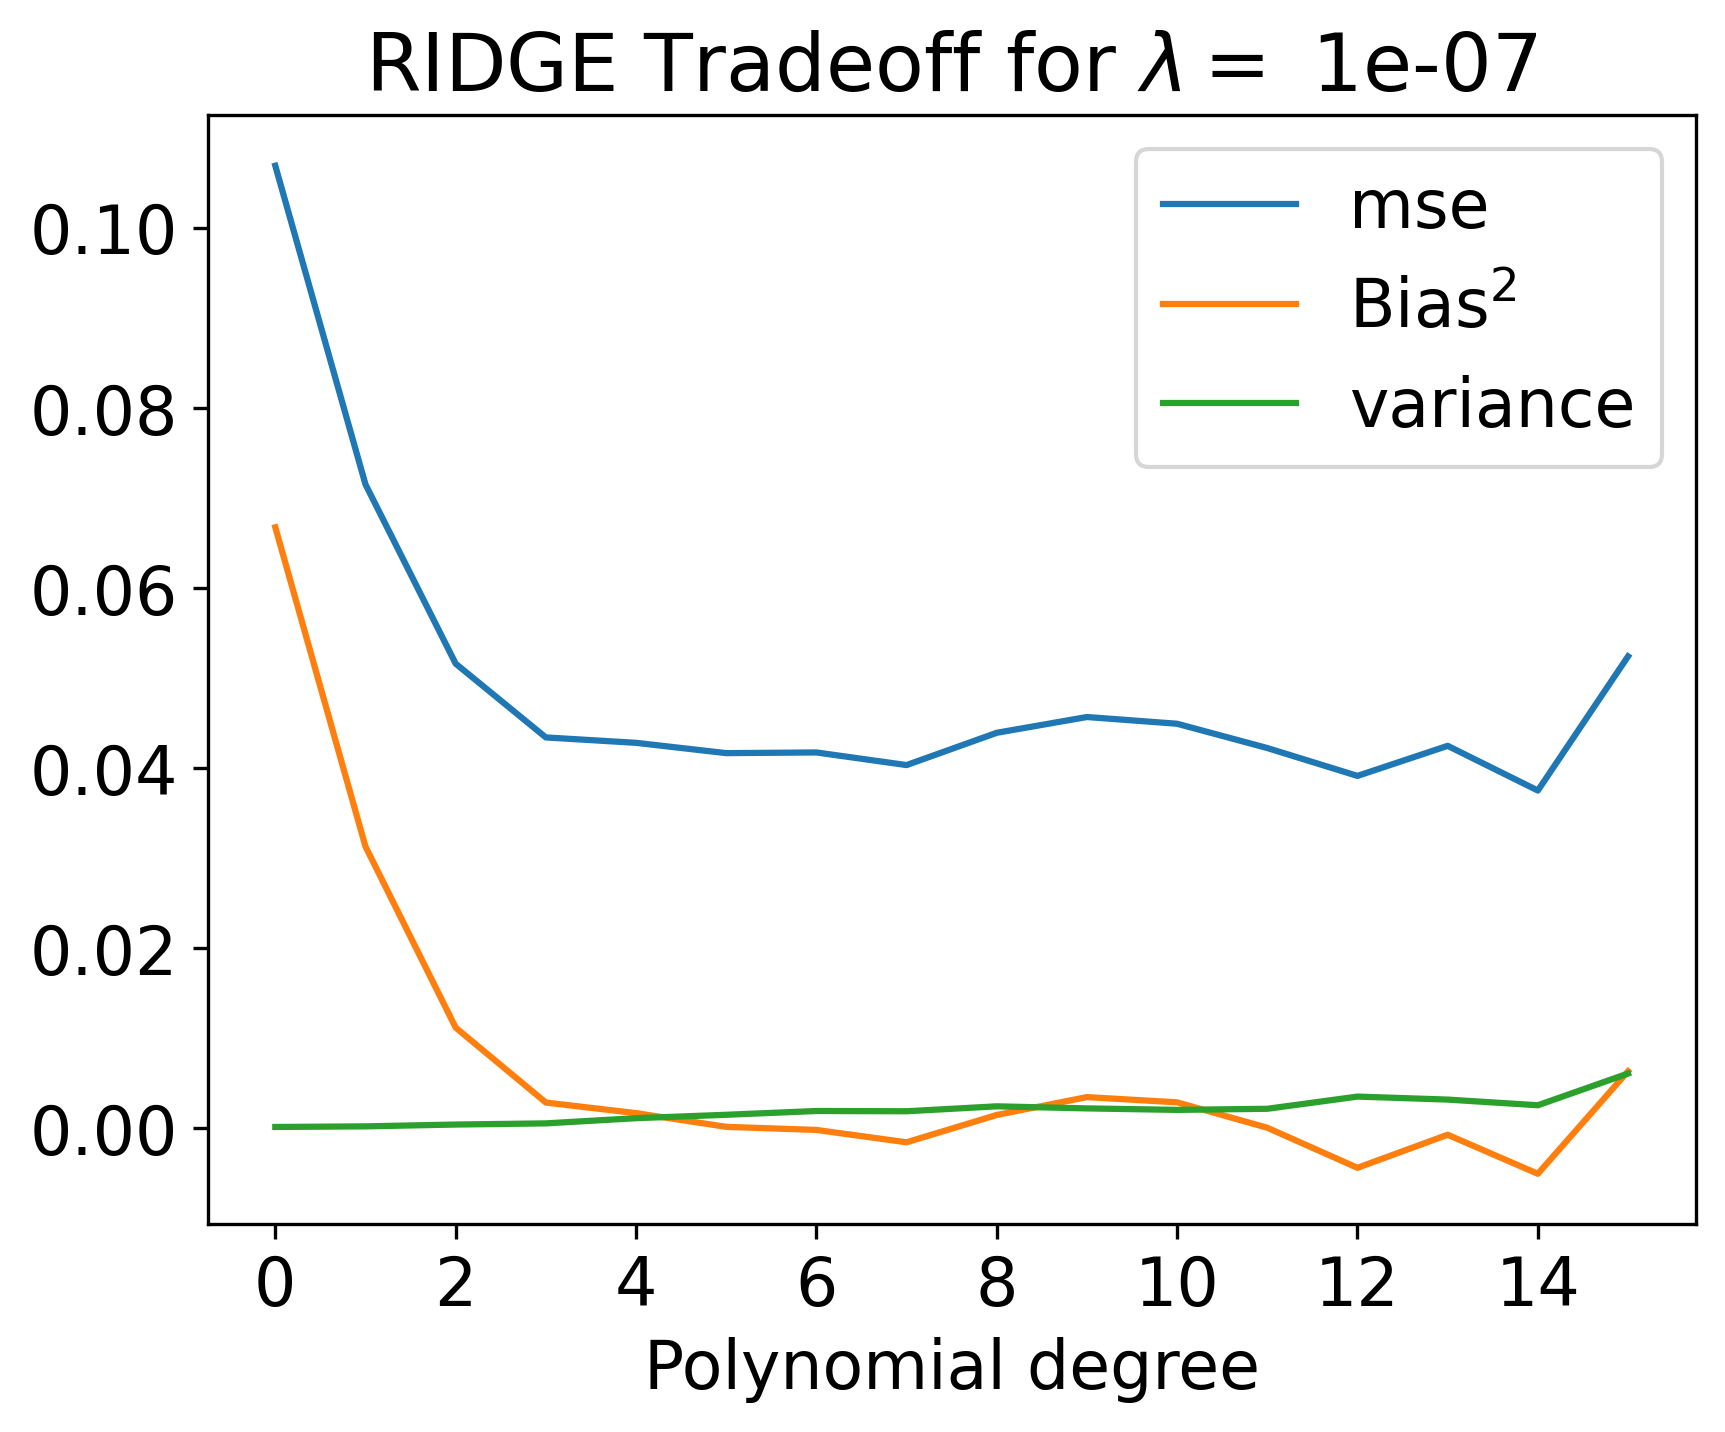
\includegraphics[width=\textwidth]{../figures/tradeoff_RIDGE_1e-07.png}
    \caption{}
    \label{fig:l_1e-07}
  \end{subfigure}
  \begin{subfigure}{.5\textwidth}
    \centering
    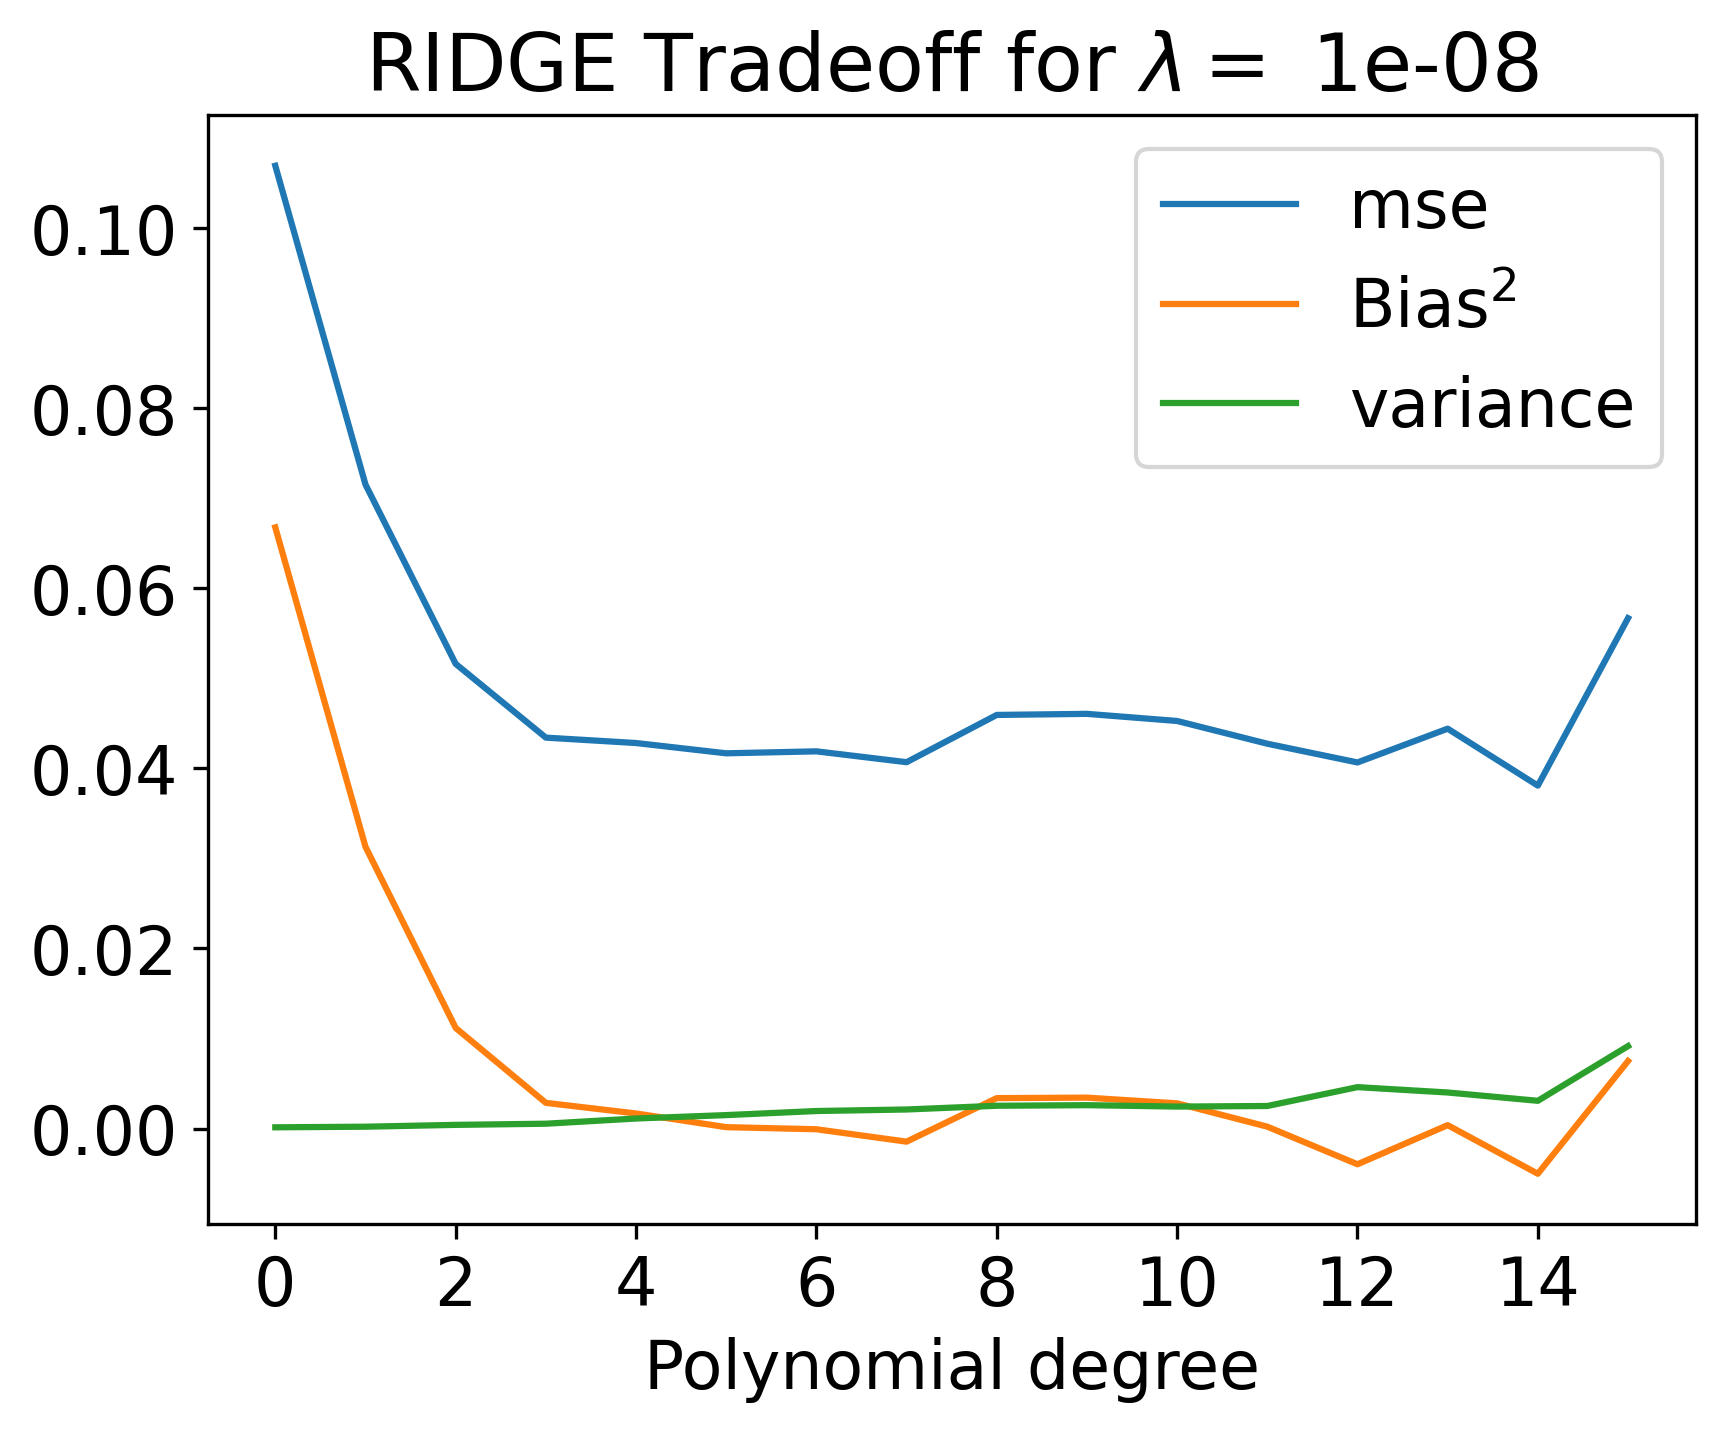
\includegraphics[width=\textwidth]{../figures/tradeoff_RIDGE_1e-08.png}
    \caption{}
    \label{fig:l_1e-08}
  \end{subfigure}
  \begin{subfigure}{.5\textwidth}
    \centering
    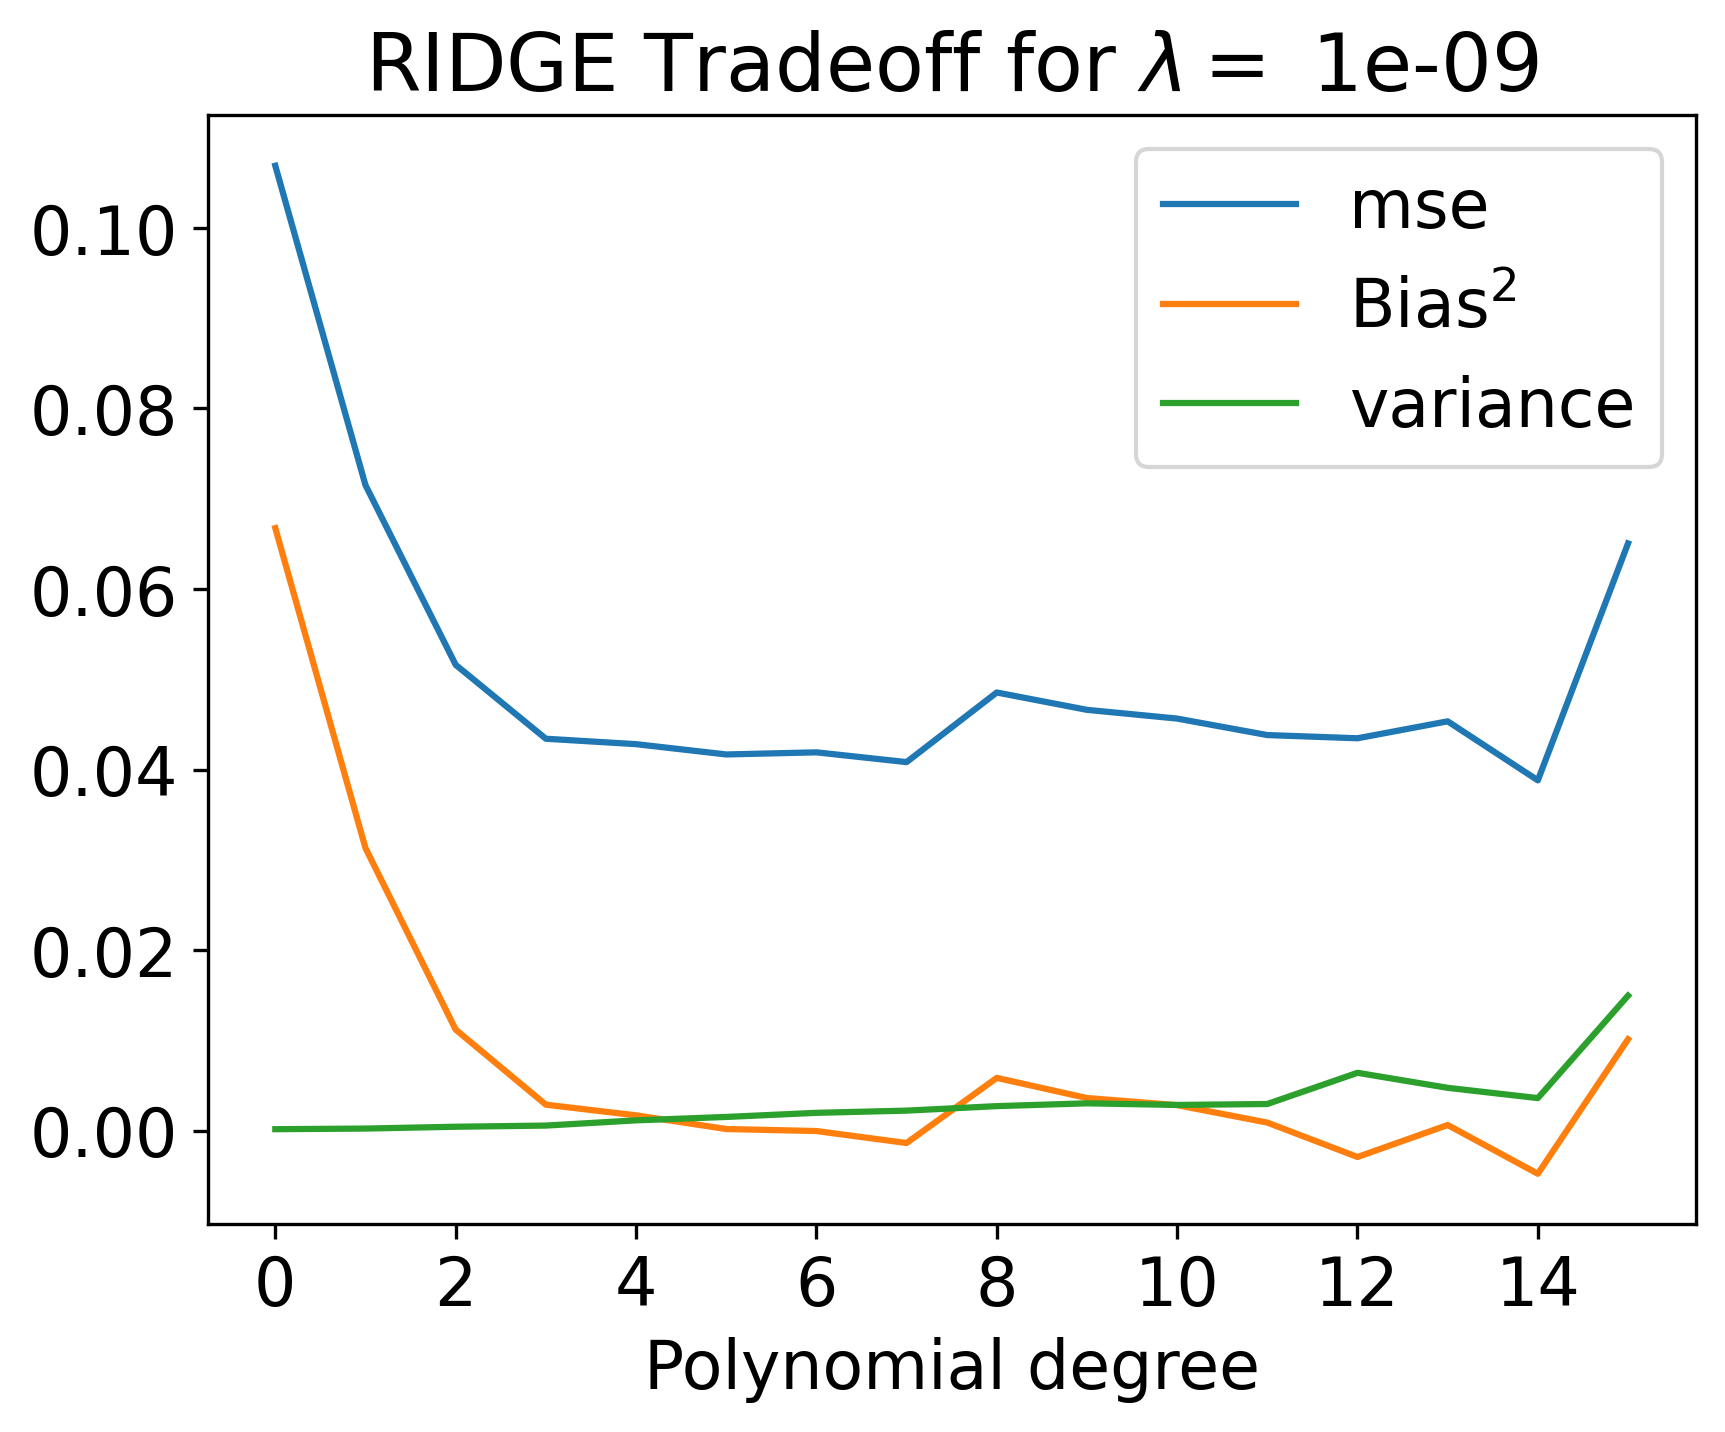
\includegraphics[width=\textwidth]{../figures/tradeoff_RIDGE_1e-09.png}
    \caption{}
    \label{fig:l_1e-09}
  \end{subfigure}
  \begin{subfigure}{.5\textwidth}
    \centering
    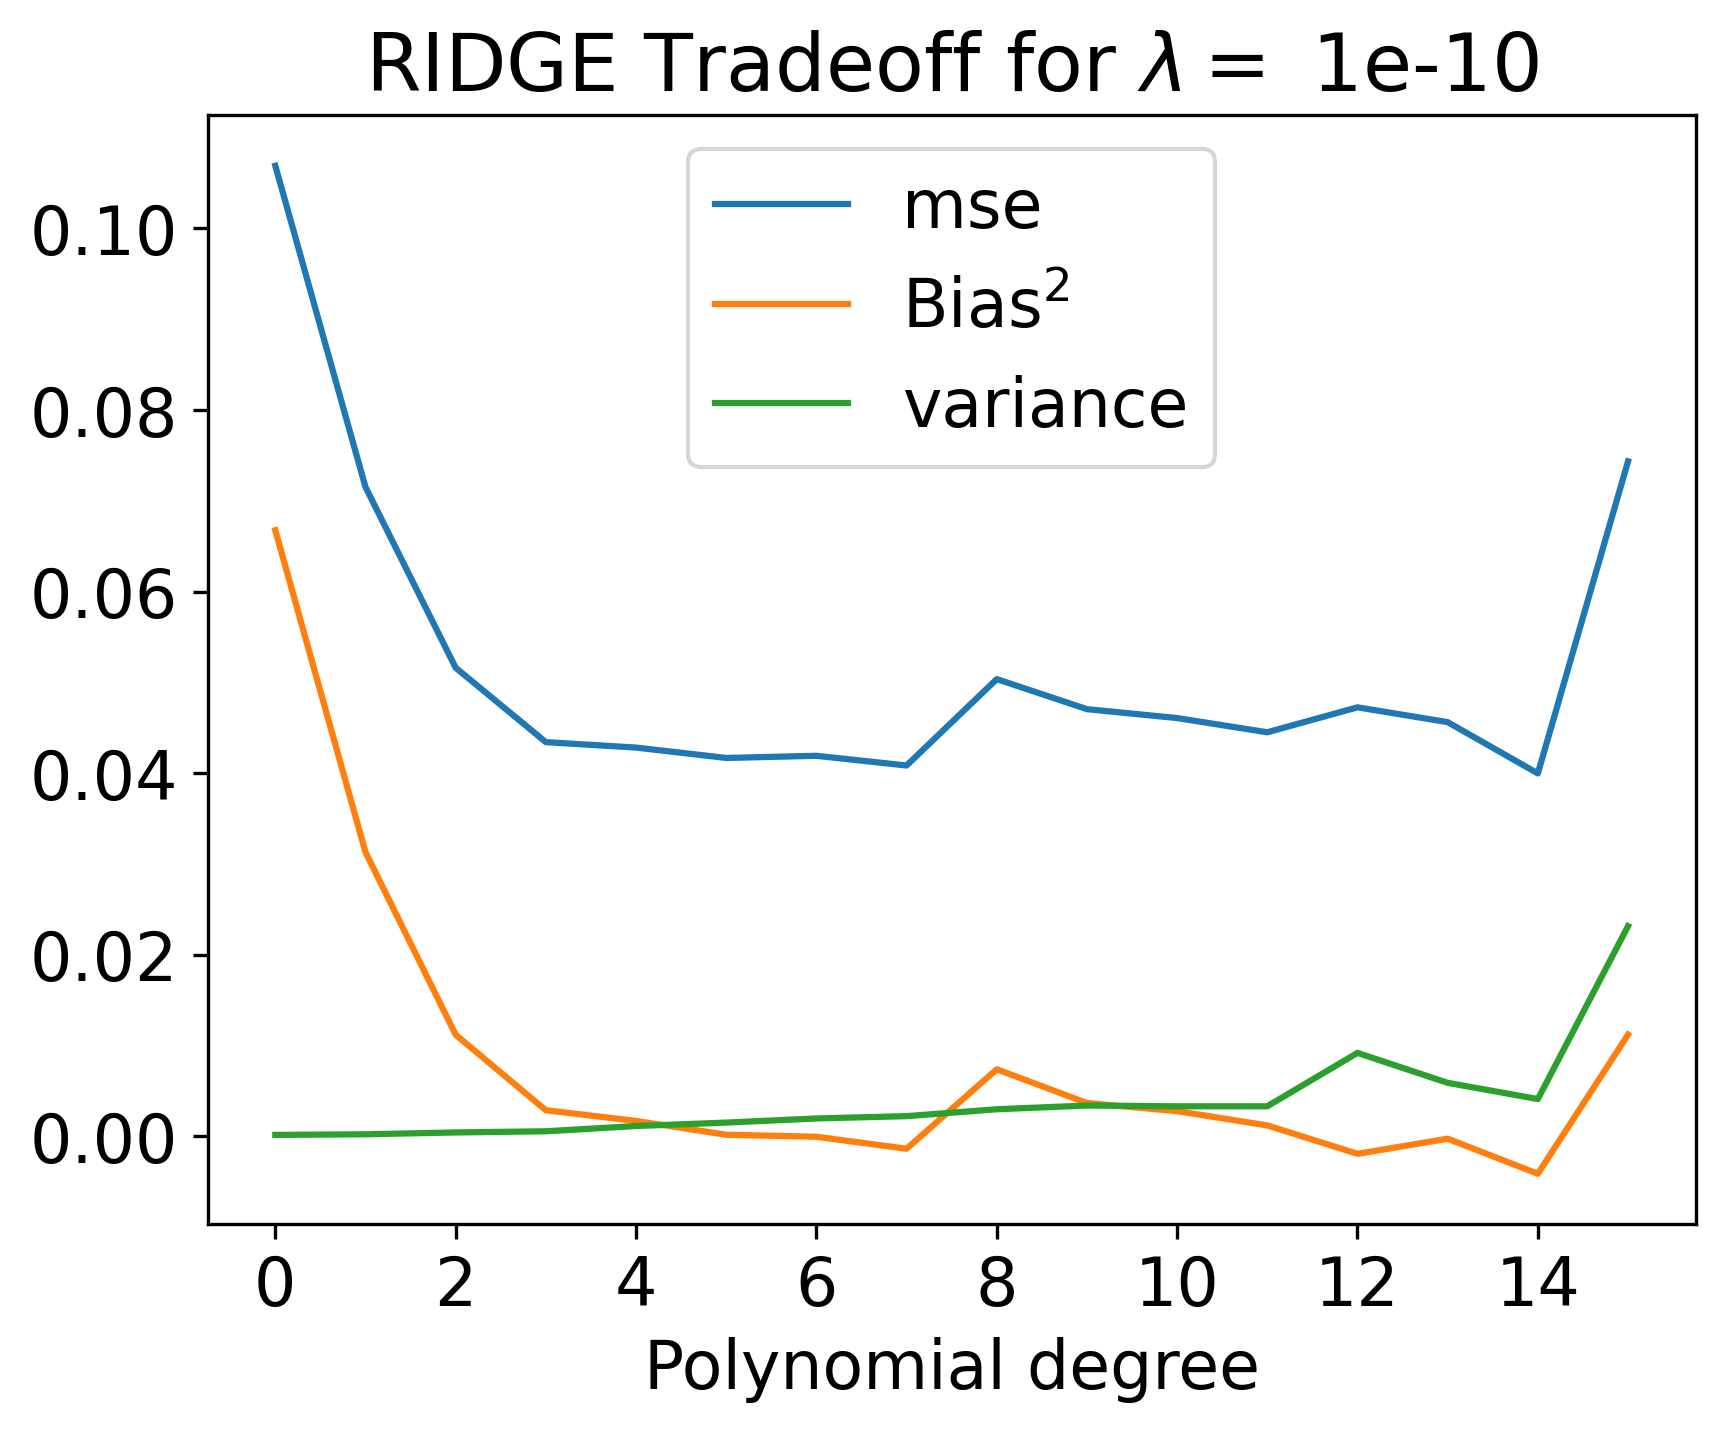
\includegraphics[width=\textwidth]{../figures/tradeoff_RIDGE_1e-10.png}
    \caption{}
    \label{fig:l_1e-10}
  \end{subfigure}
  \begin{subfigure}{.5\textwidth}
    \centering
    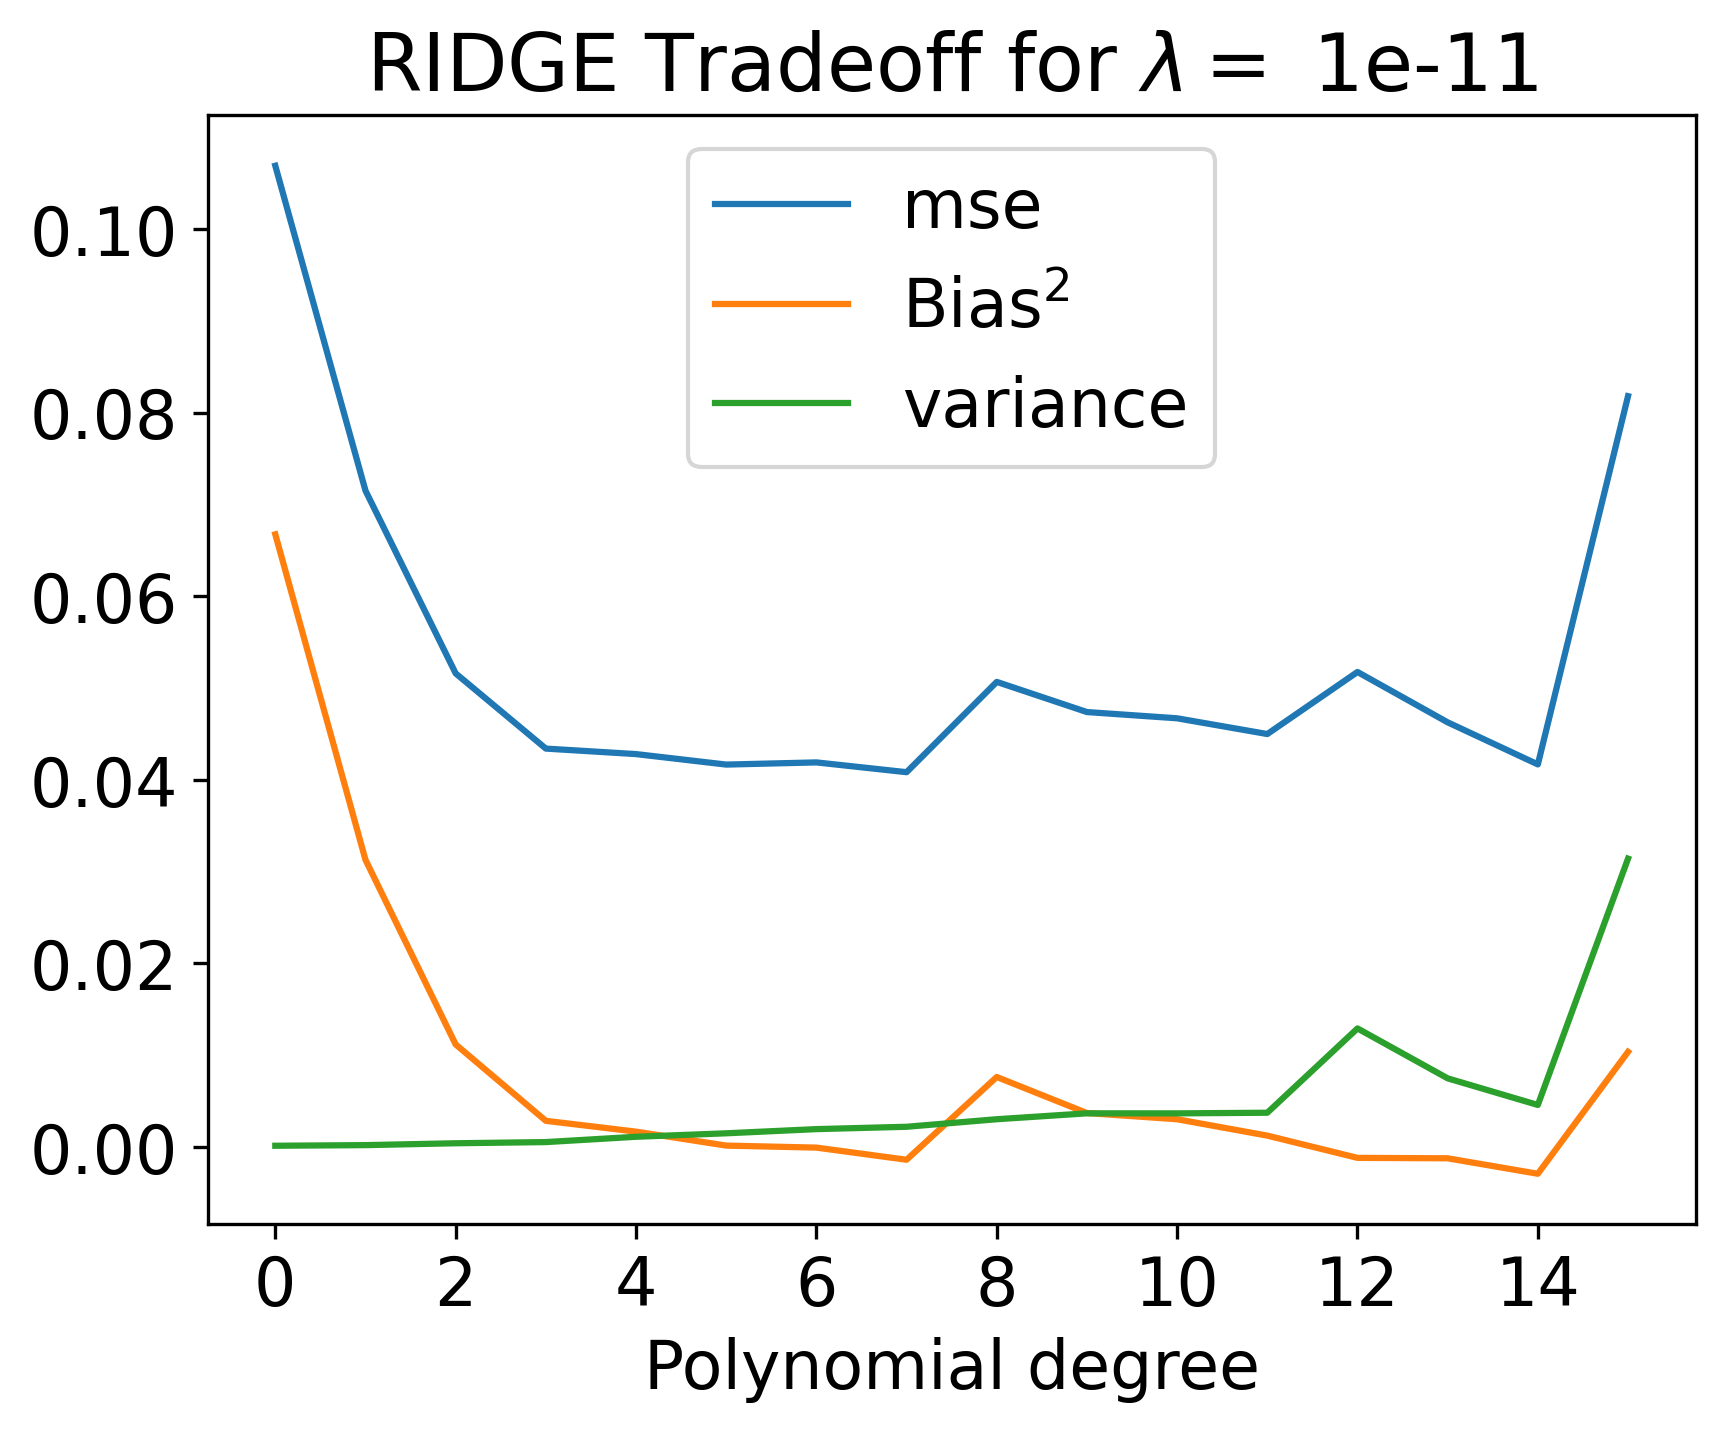
\includegraphics[width=\textwidth]{../figures/tradeoff_RIDGE_1e-11.png}
    \caption{}
    \label{fig:l_1e-11}
  \end{subfigure}
  \begin{subfigure}{.5\textwidth}
    \centering
    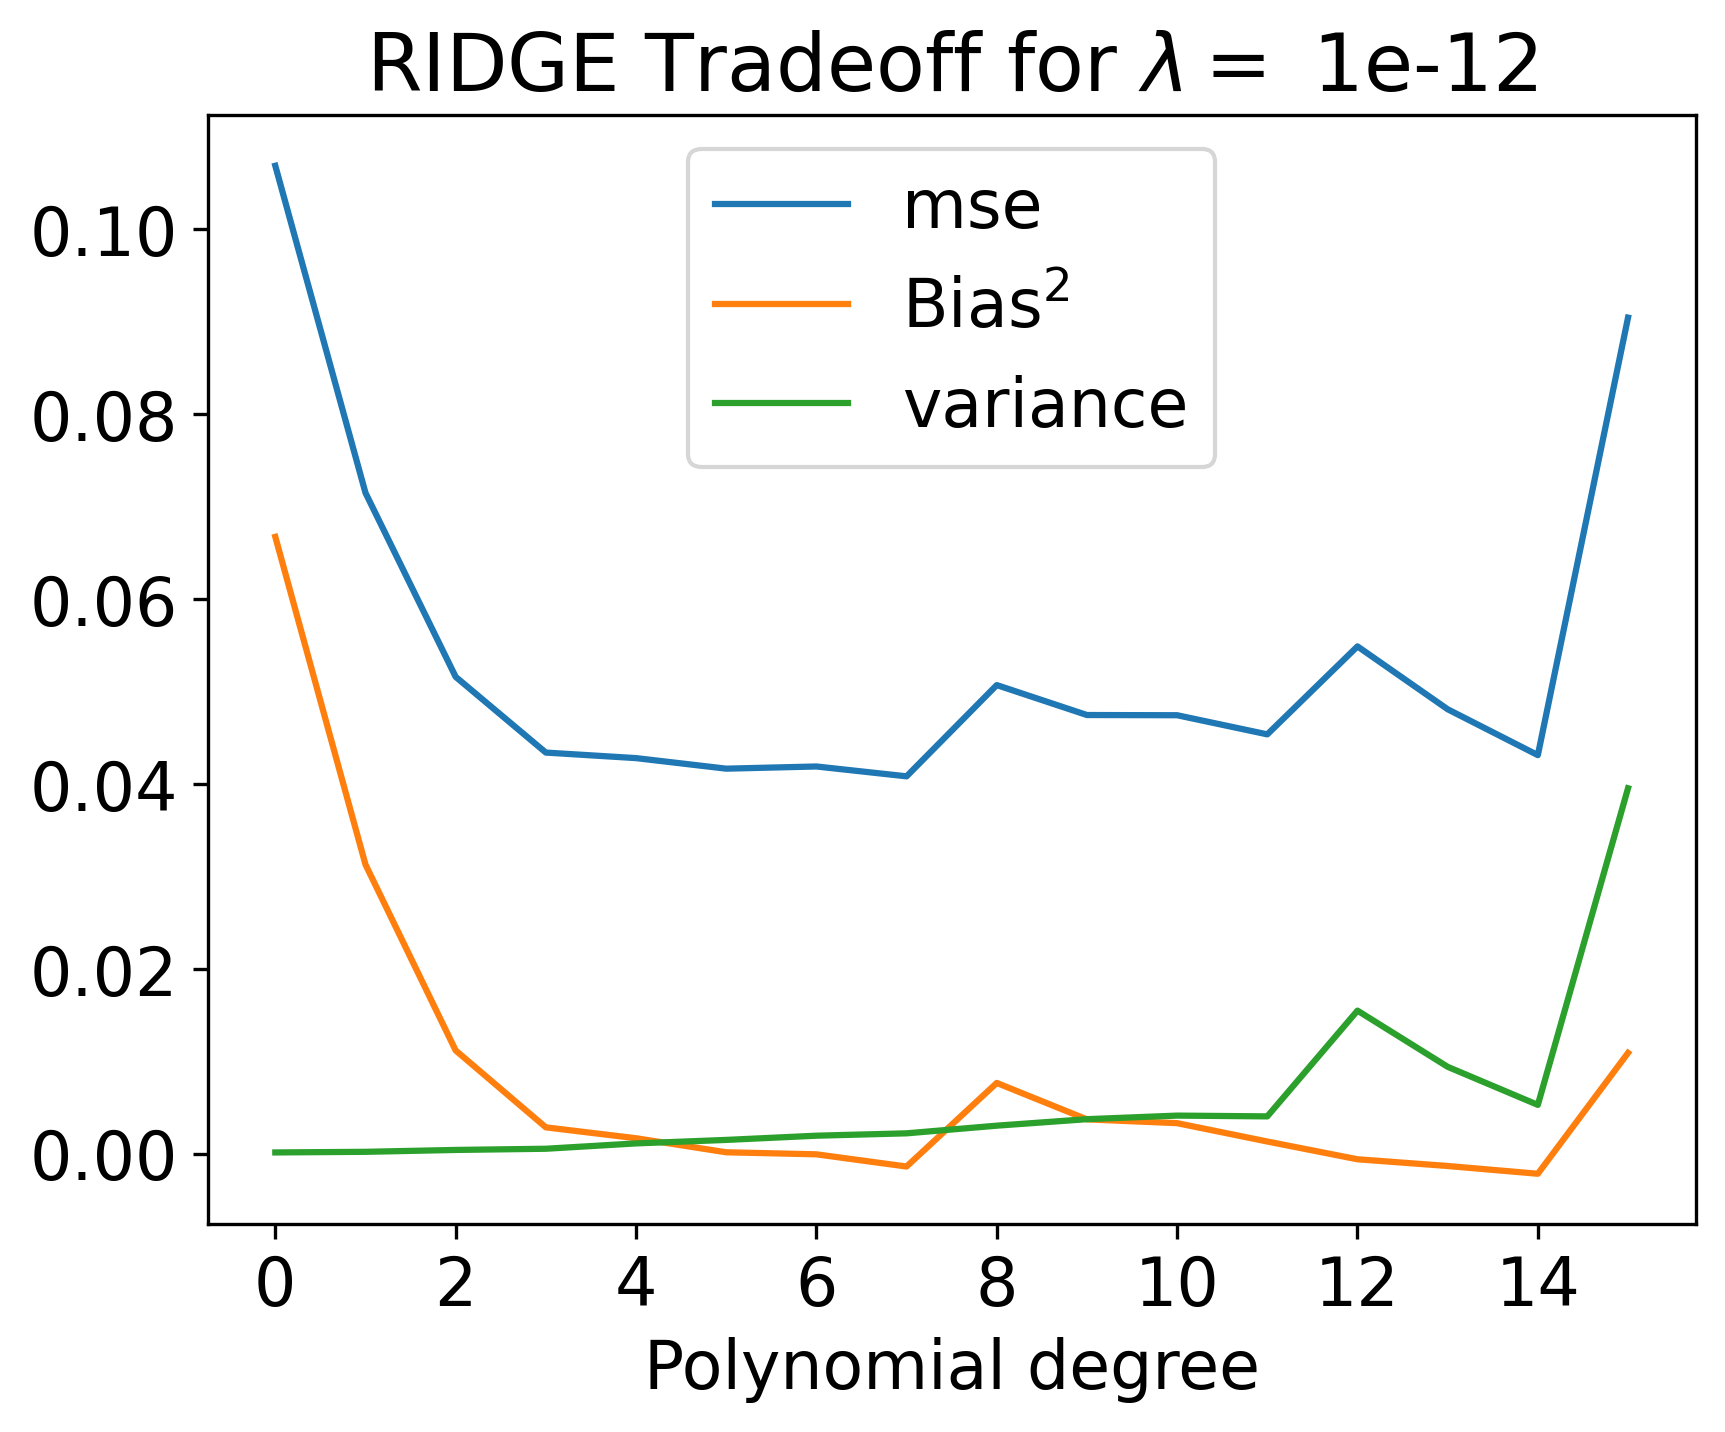
\includegraphics[width=\textwidth]{../figures/tradeoff_RIDGE_1e-12.png}
    \caption{}
    \label{fig:l_1e-12}
  \end{subfigure}
  \caption{Bias variance tradeoff for different choices of lambda using Ridge regression for data with $n=30$ steps and noise standard deviation of $\sigma=0.2$}
  \label{fig:ridge_tradeoff}
\end{figure}
\begin{figure}[H]
  \begin{subfigure}{.5\textwidth}
    \centering
    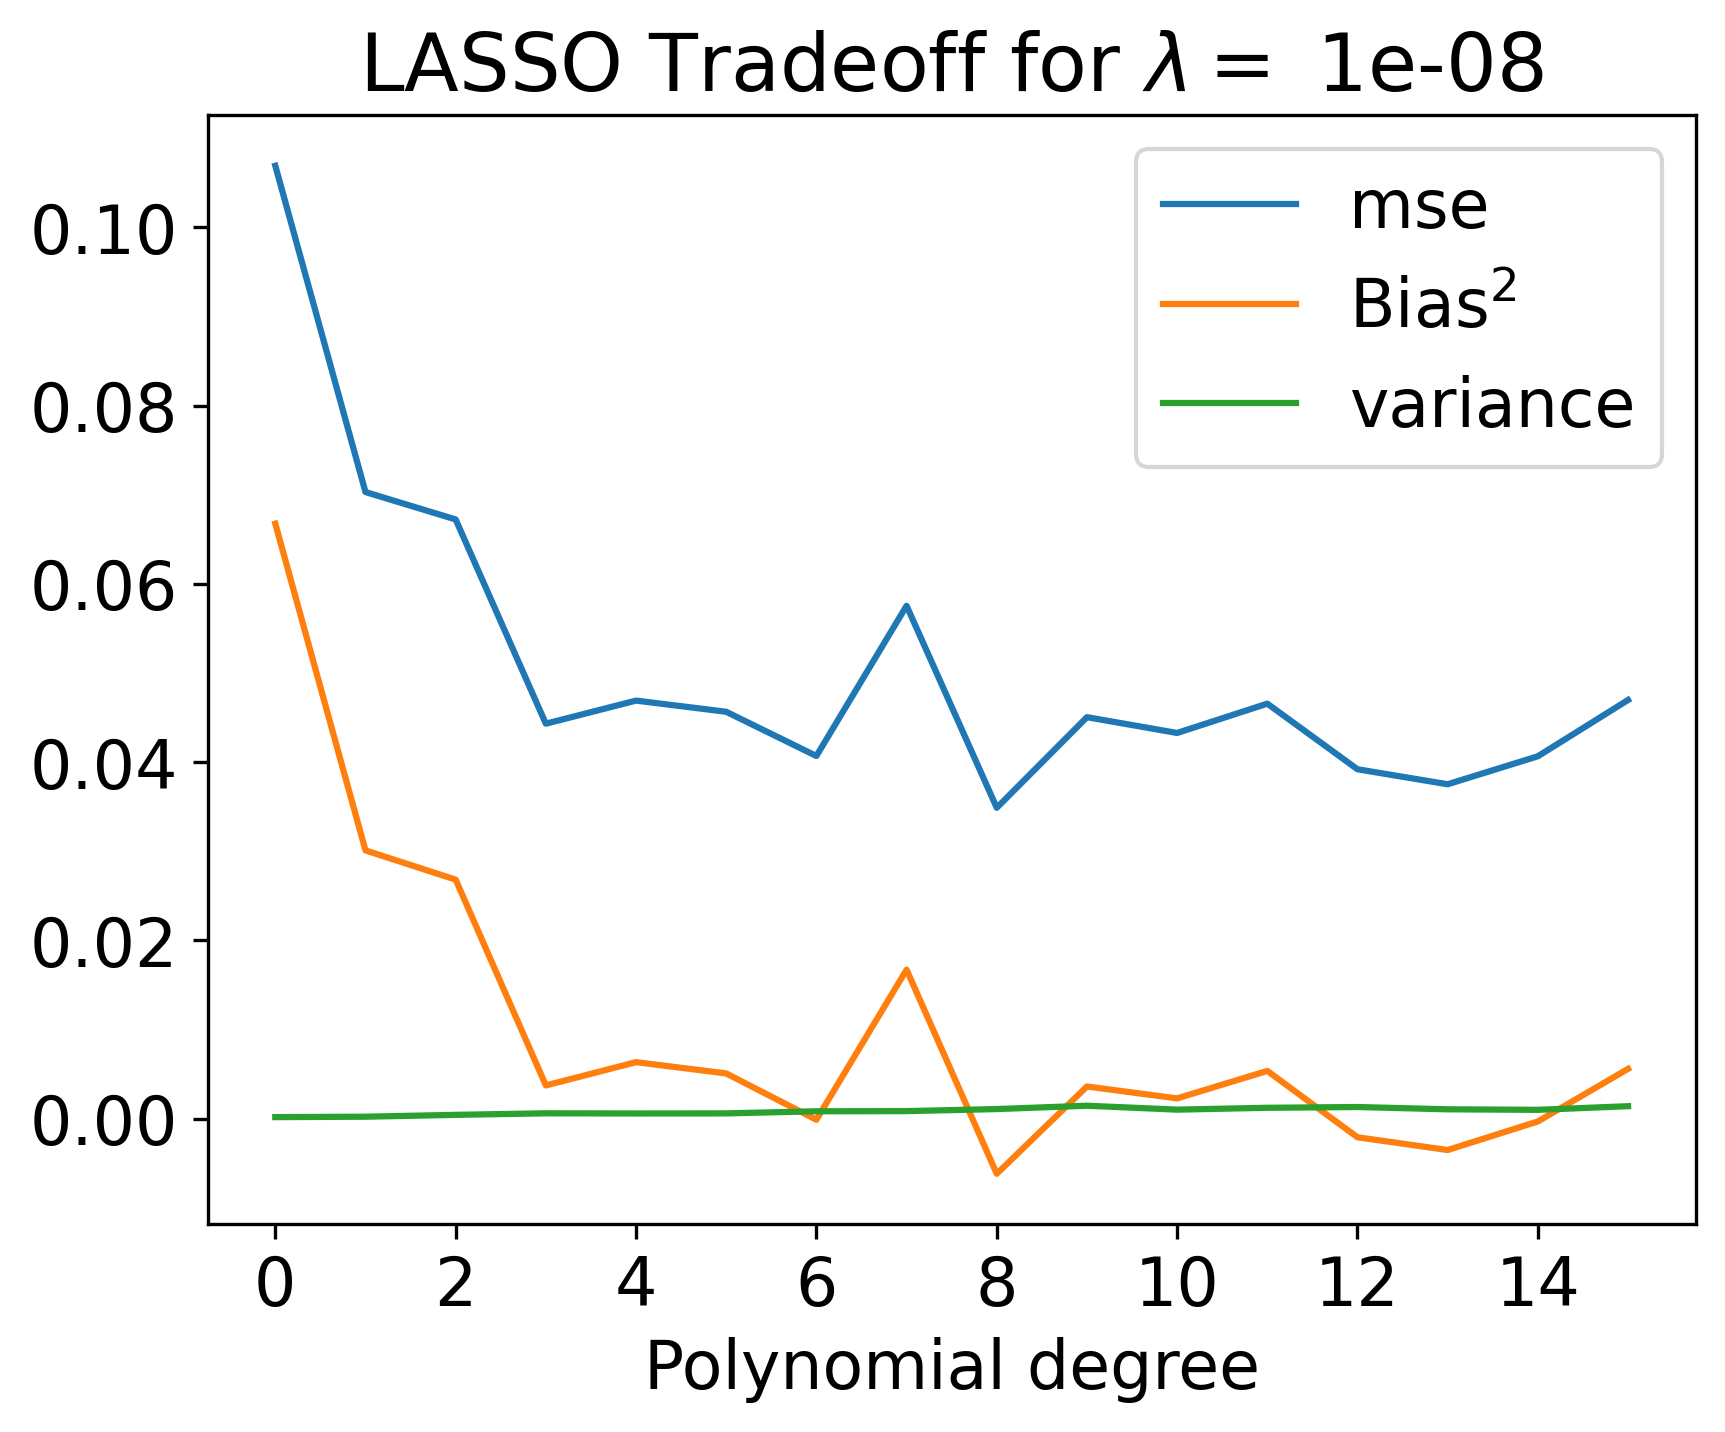
\includegraphics[width=\textwidth]{../figures/tradeoff_LASSO_1e-08.png}
    \caption{}
    \label{fig:l_1e-08}
  \end{subfigure}
  \begin{subfigure}{.5\textwidth}
    \centering
    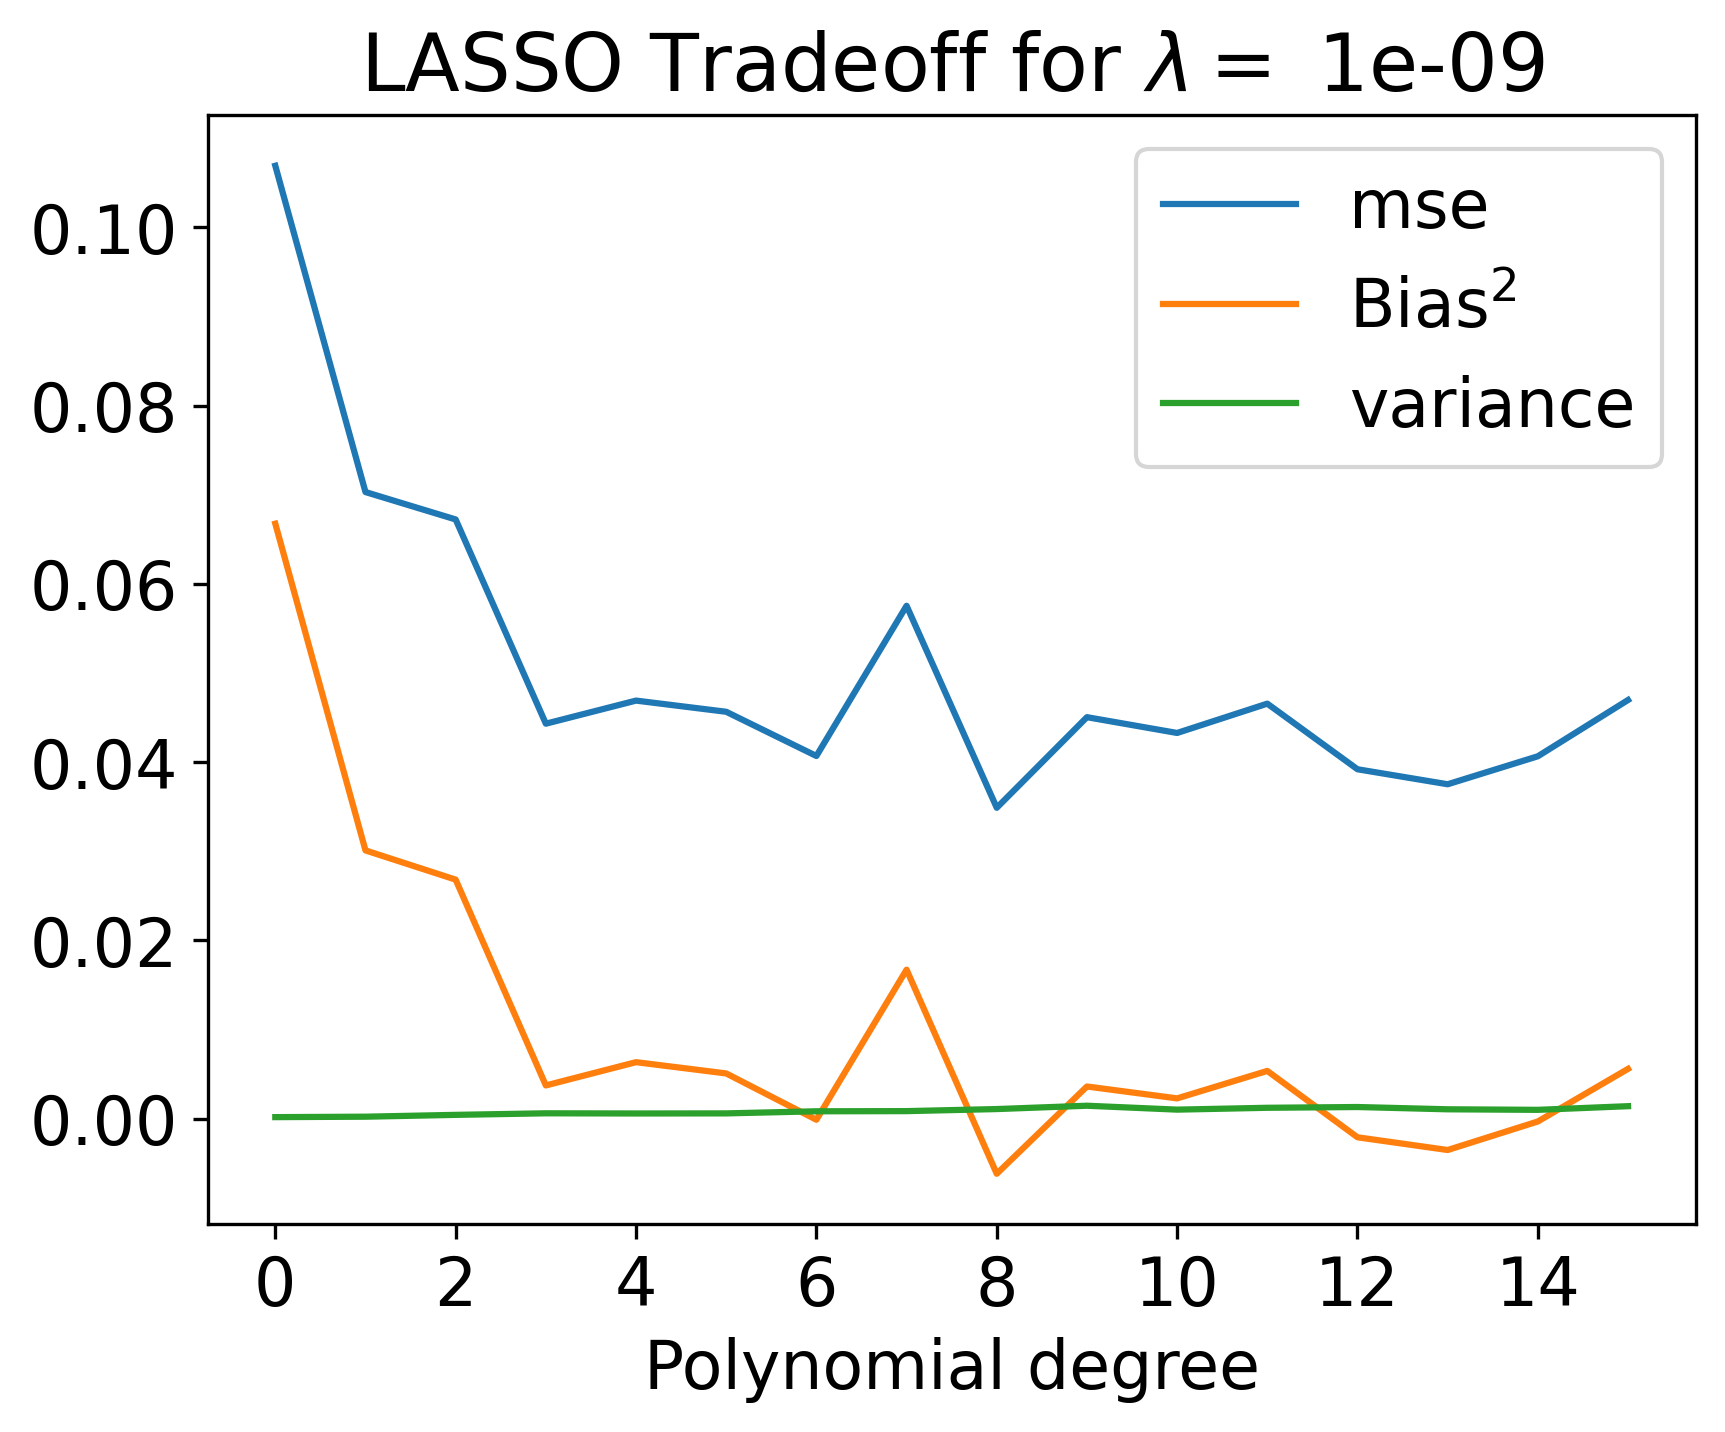
\includegraphics[width=\textwidth]{../figures/tradeoff_LASSO_1e-09.png}
    \caption{}
    \label{fig:l_1e-09}
  \end{subfigure}
  \begin{subfigure}{.5\textwidth}
    \centering
    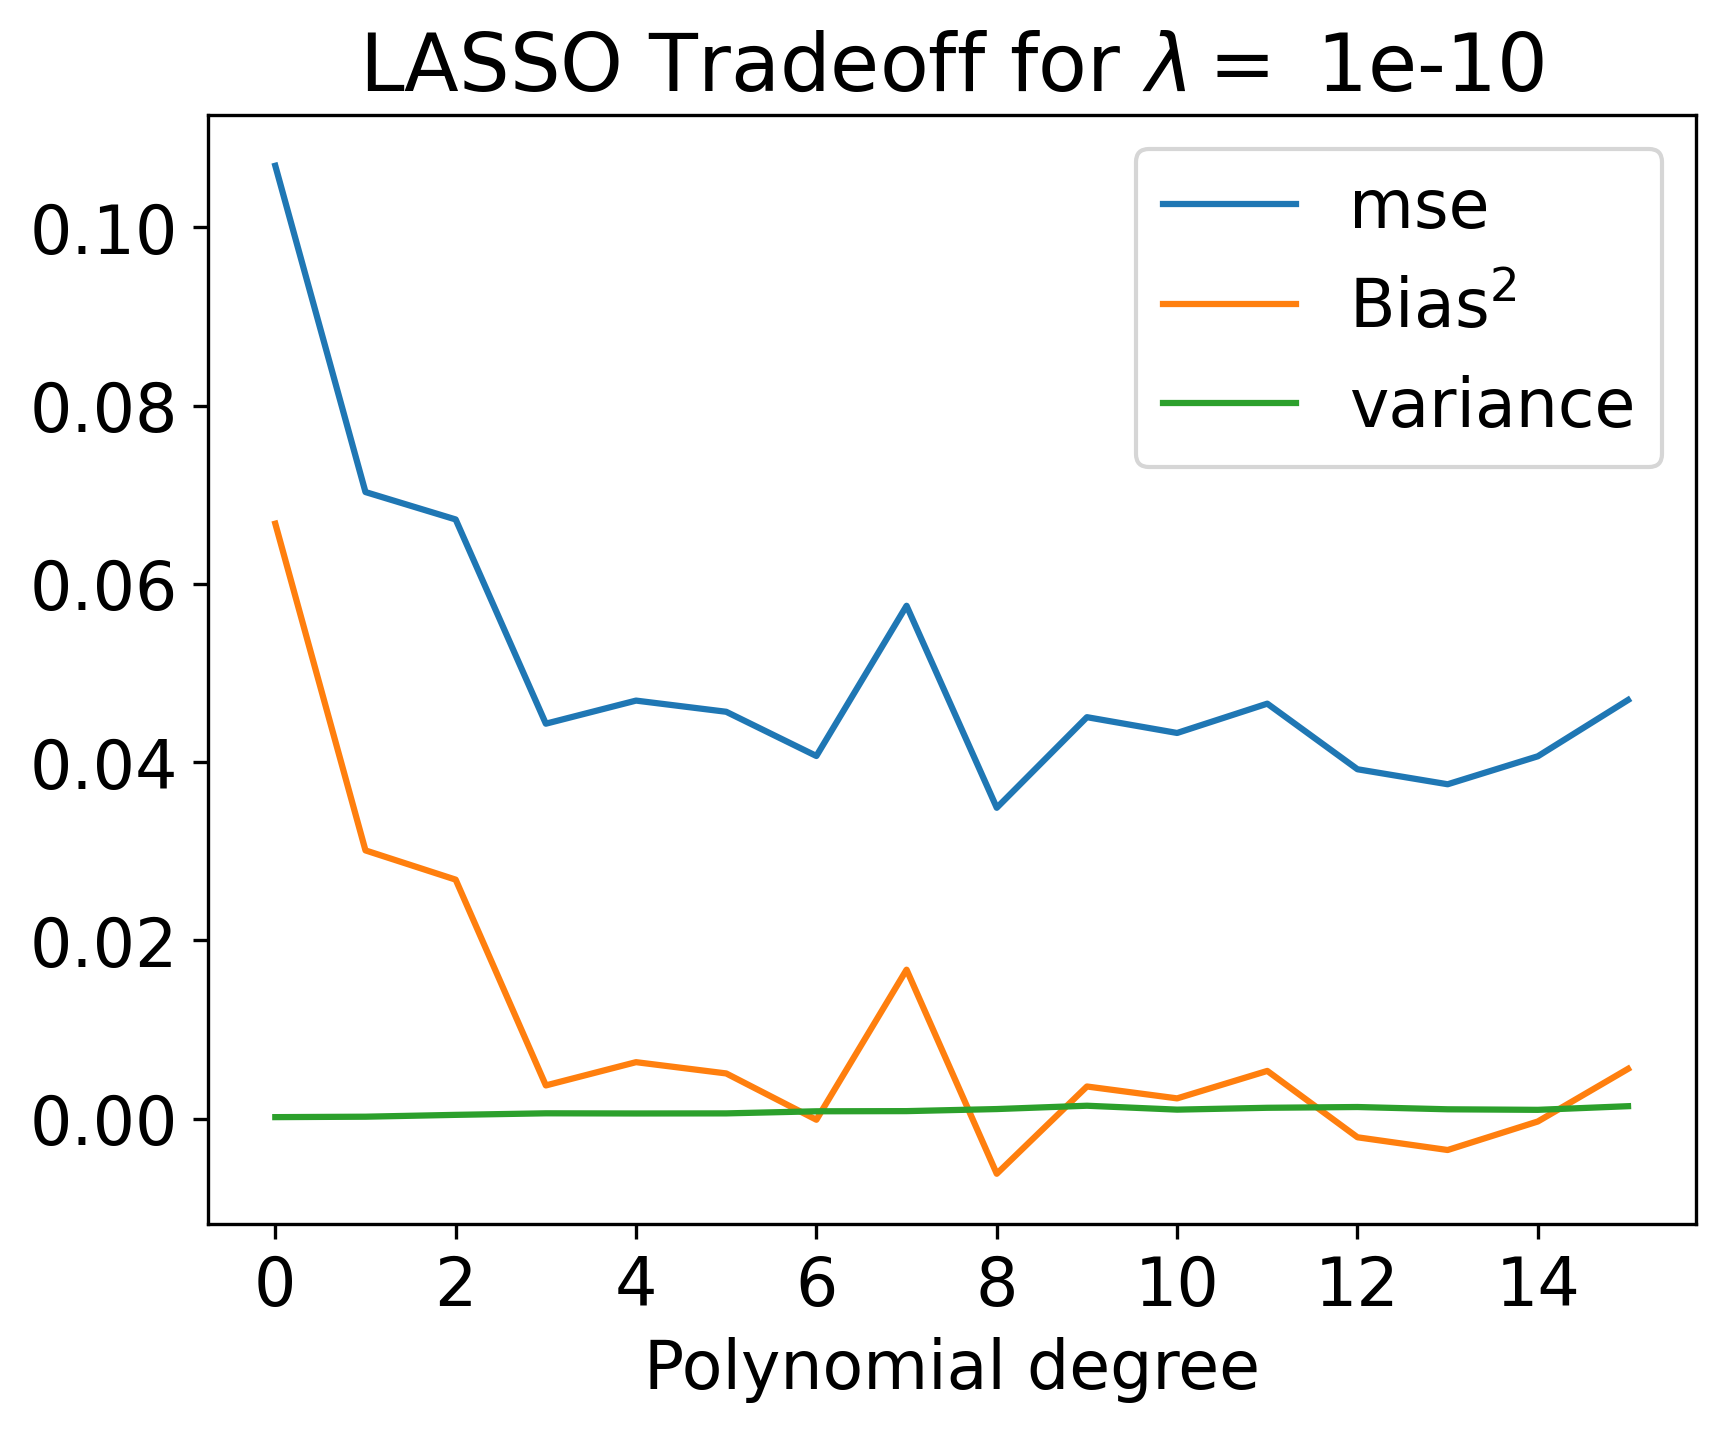
\includegraphics[width=\textwidth]{../figures/tradeoff_LASSO_1e-10.png}
    \caption{}
    \label{fig:l_1e-10}
  \end{subfigure}
  \begin{subfigure}{.5\textwidth}
    \centering
    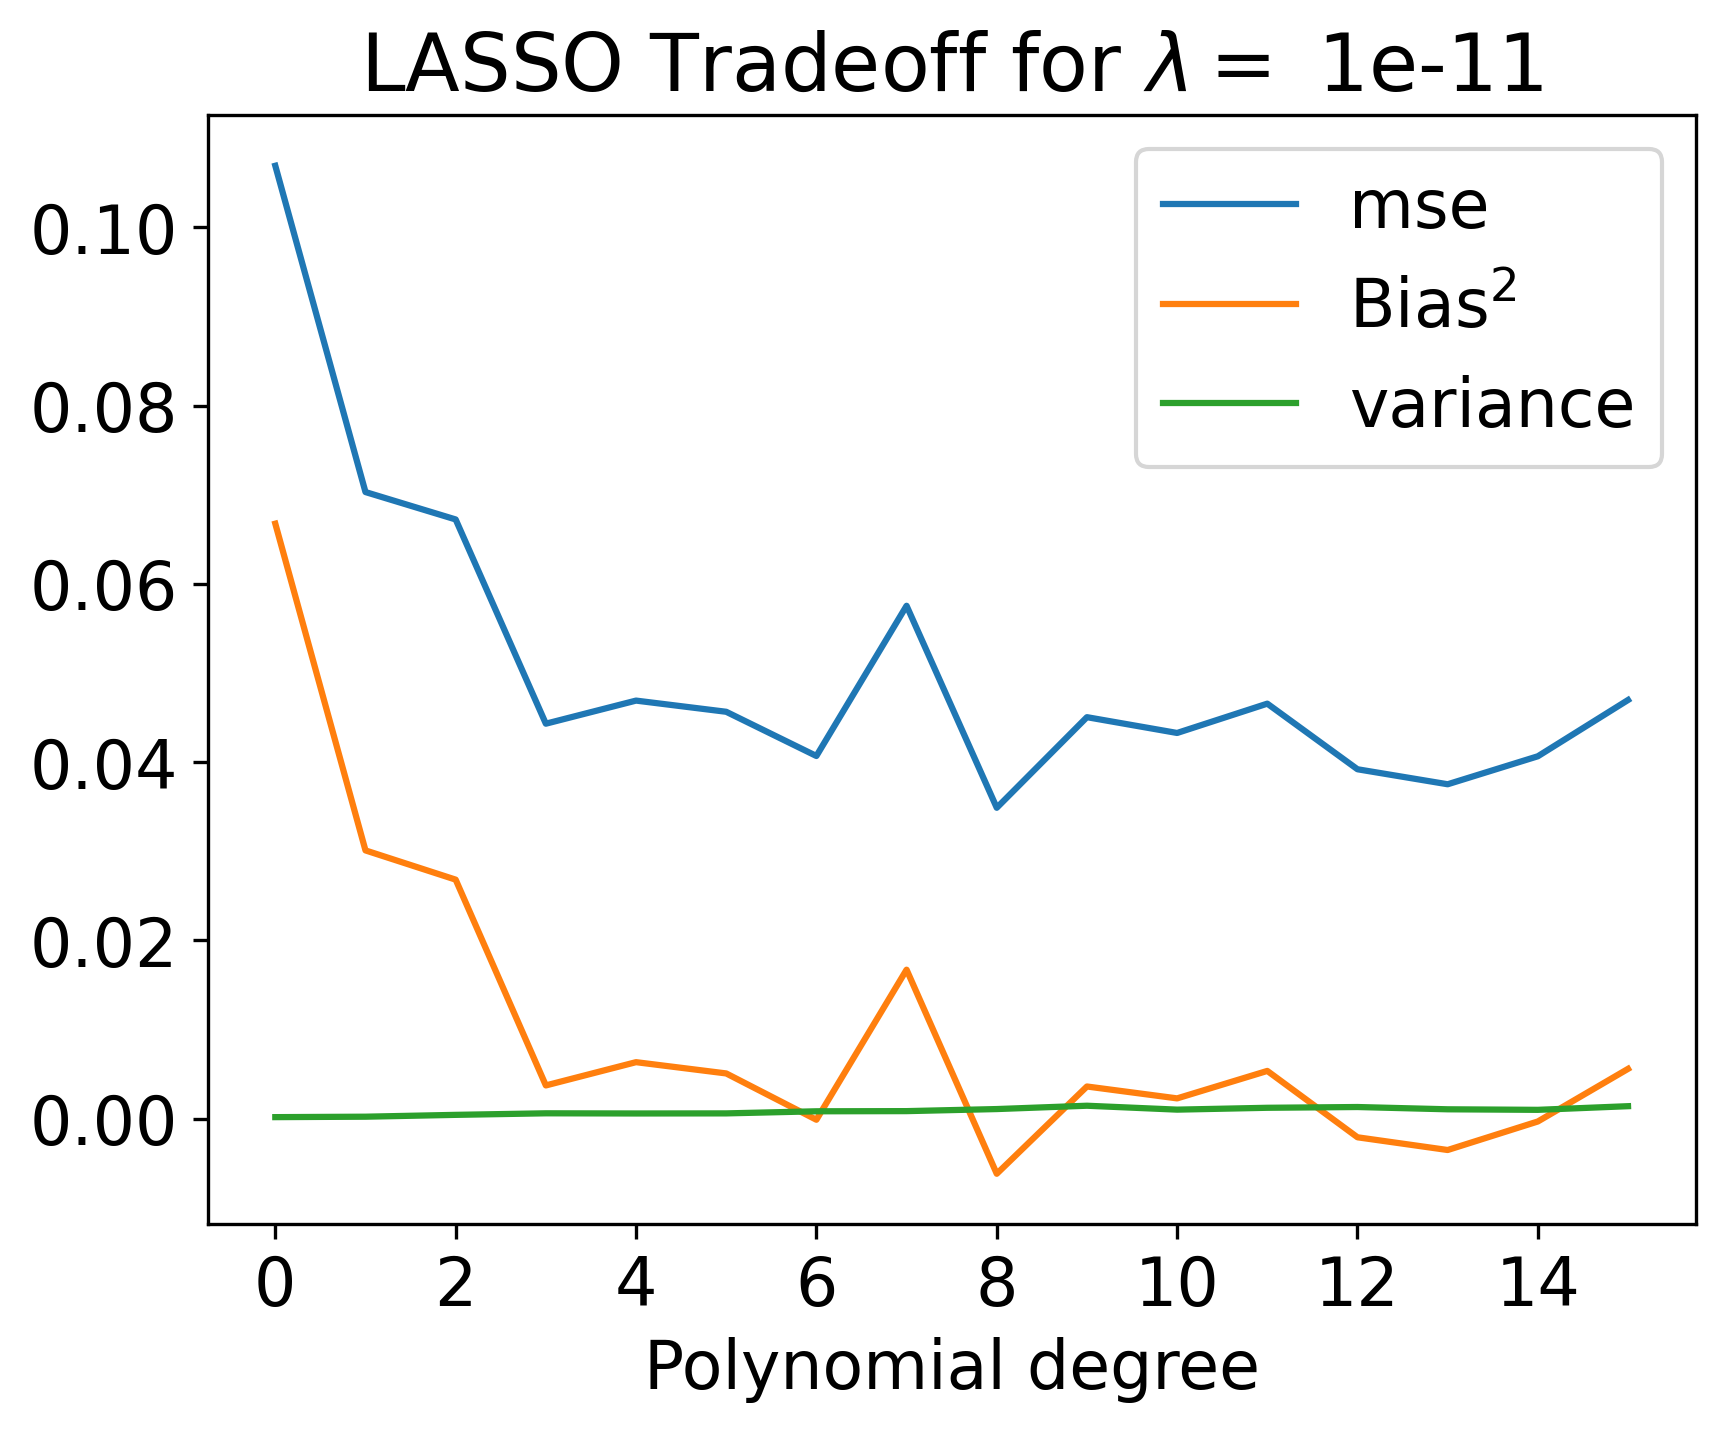
\includegraphics[width=\textwidth]{../figures/tradeoff_LASSO_1e-11.png}
    \caption{}
    \label{fig:l_1e-1}
  \end{subfigure}
  \begin{subfigure}{.5\textwidth}
    \centering
    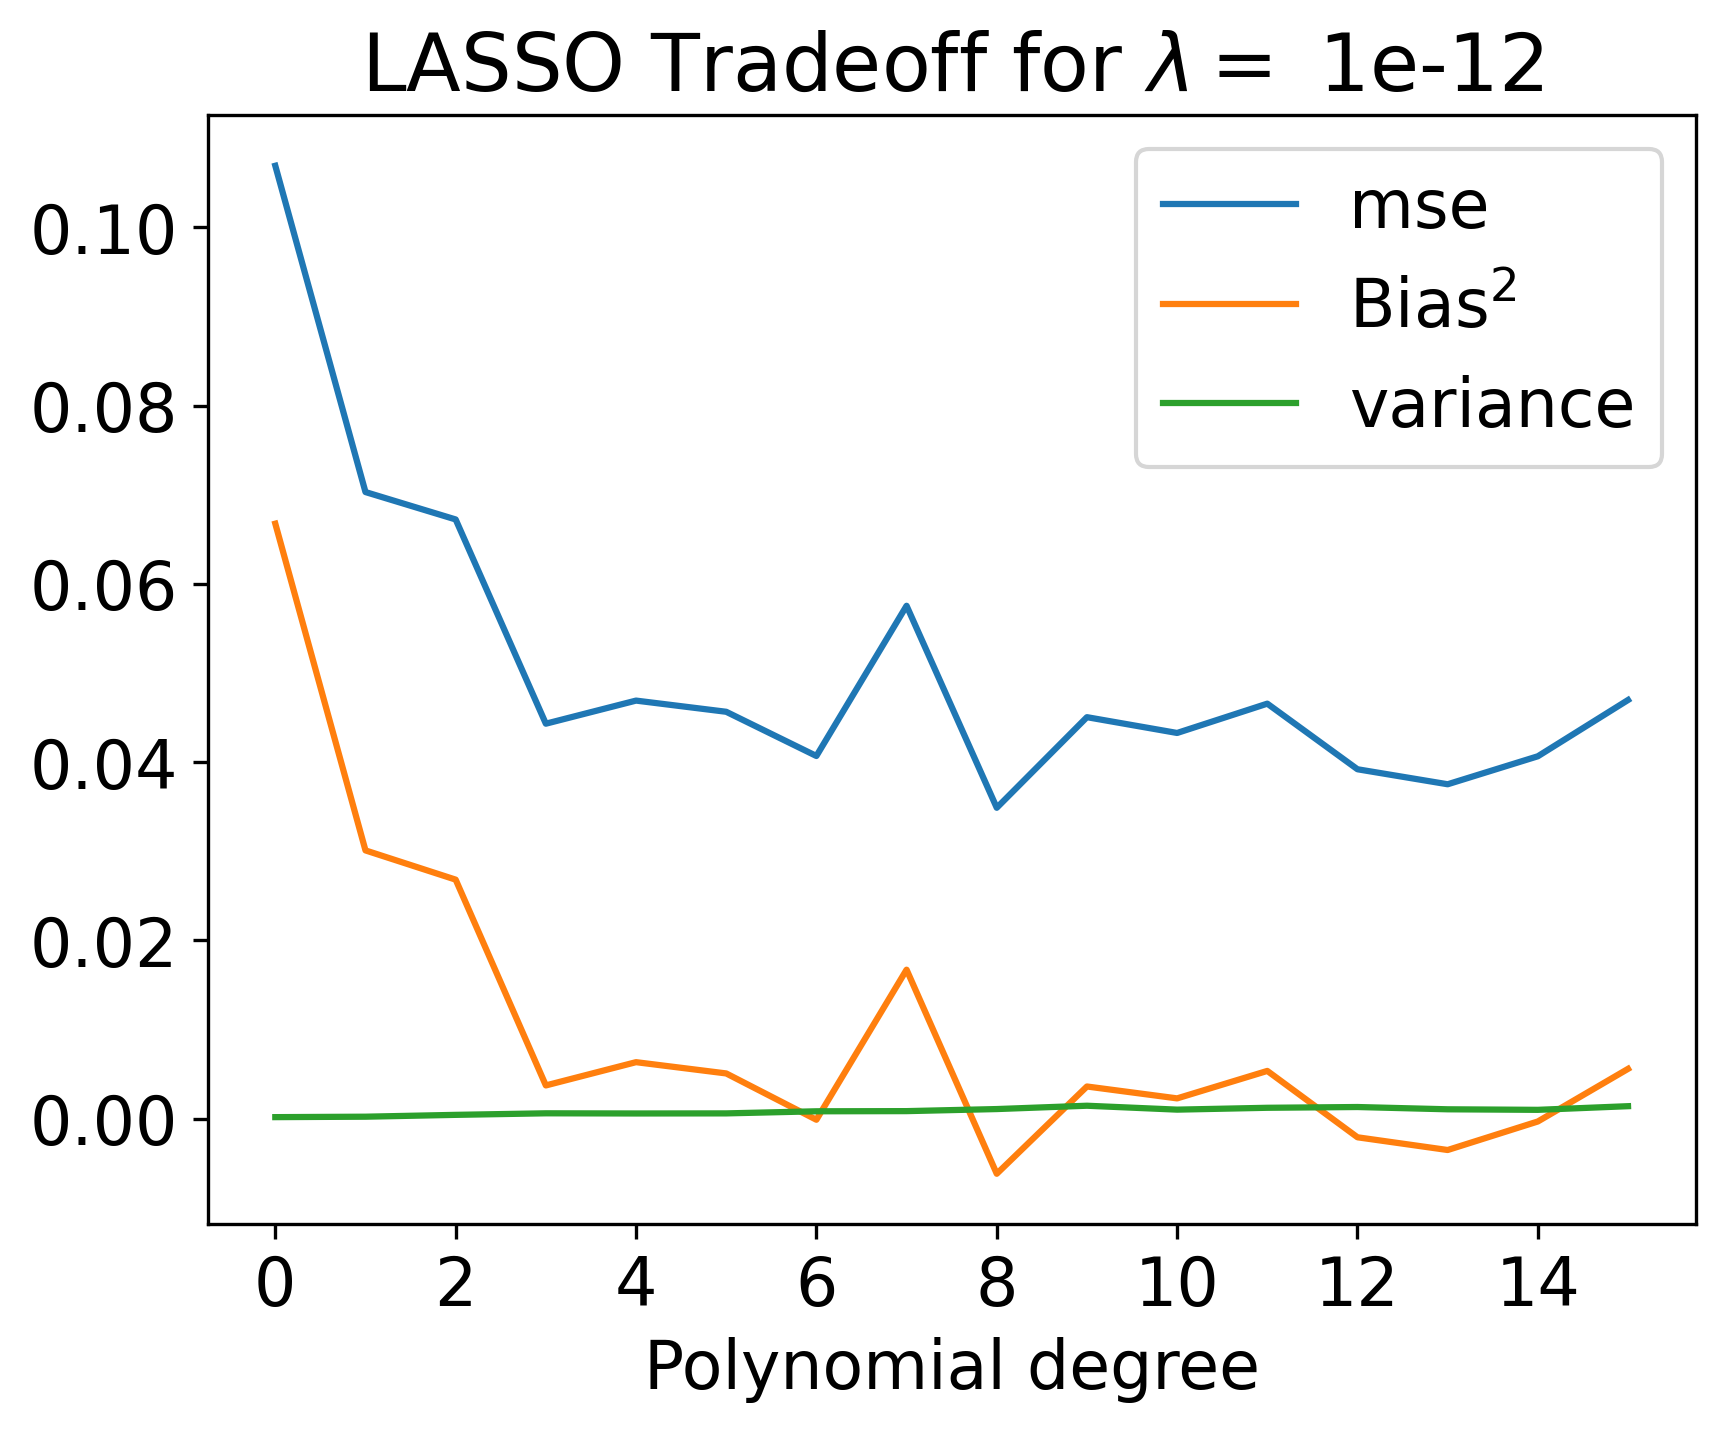
\includegraphics[width=\textwidth]{../figures/tradeoff_LASSO_1e-12.png}
    \caption{}
    \label{fig:l_1e-12}
  \end{subfigure}
  \begin{subfigure}{.5\textwidth}
    \centering
    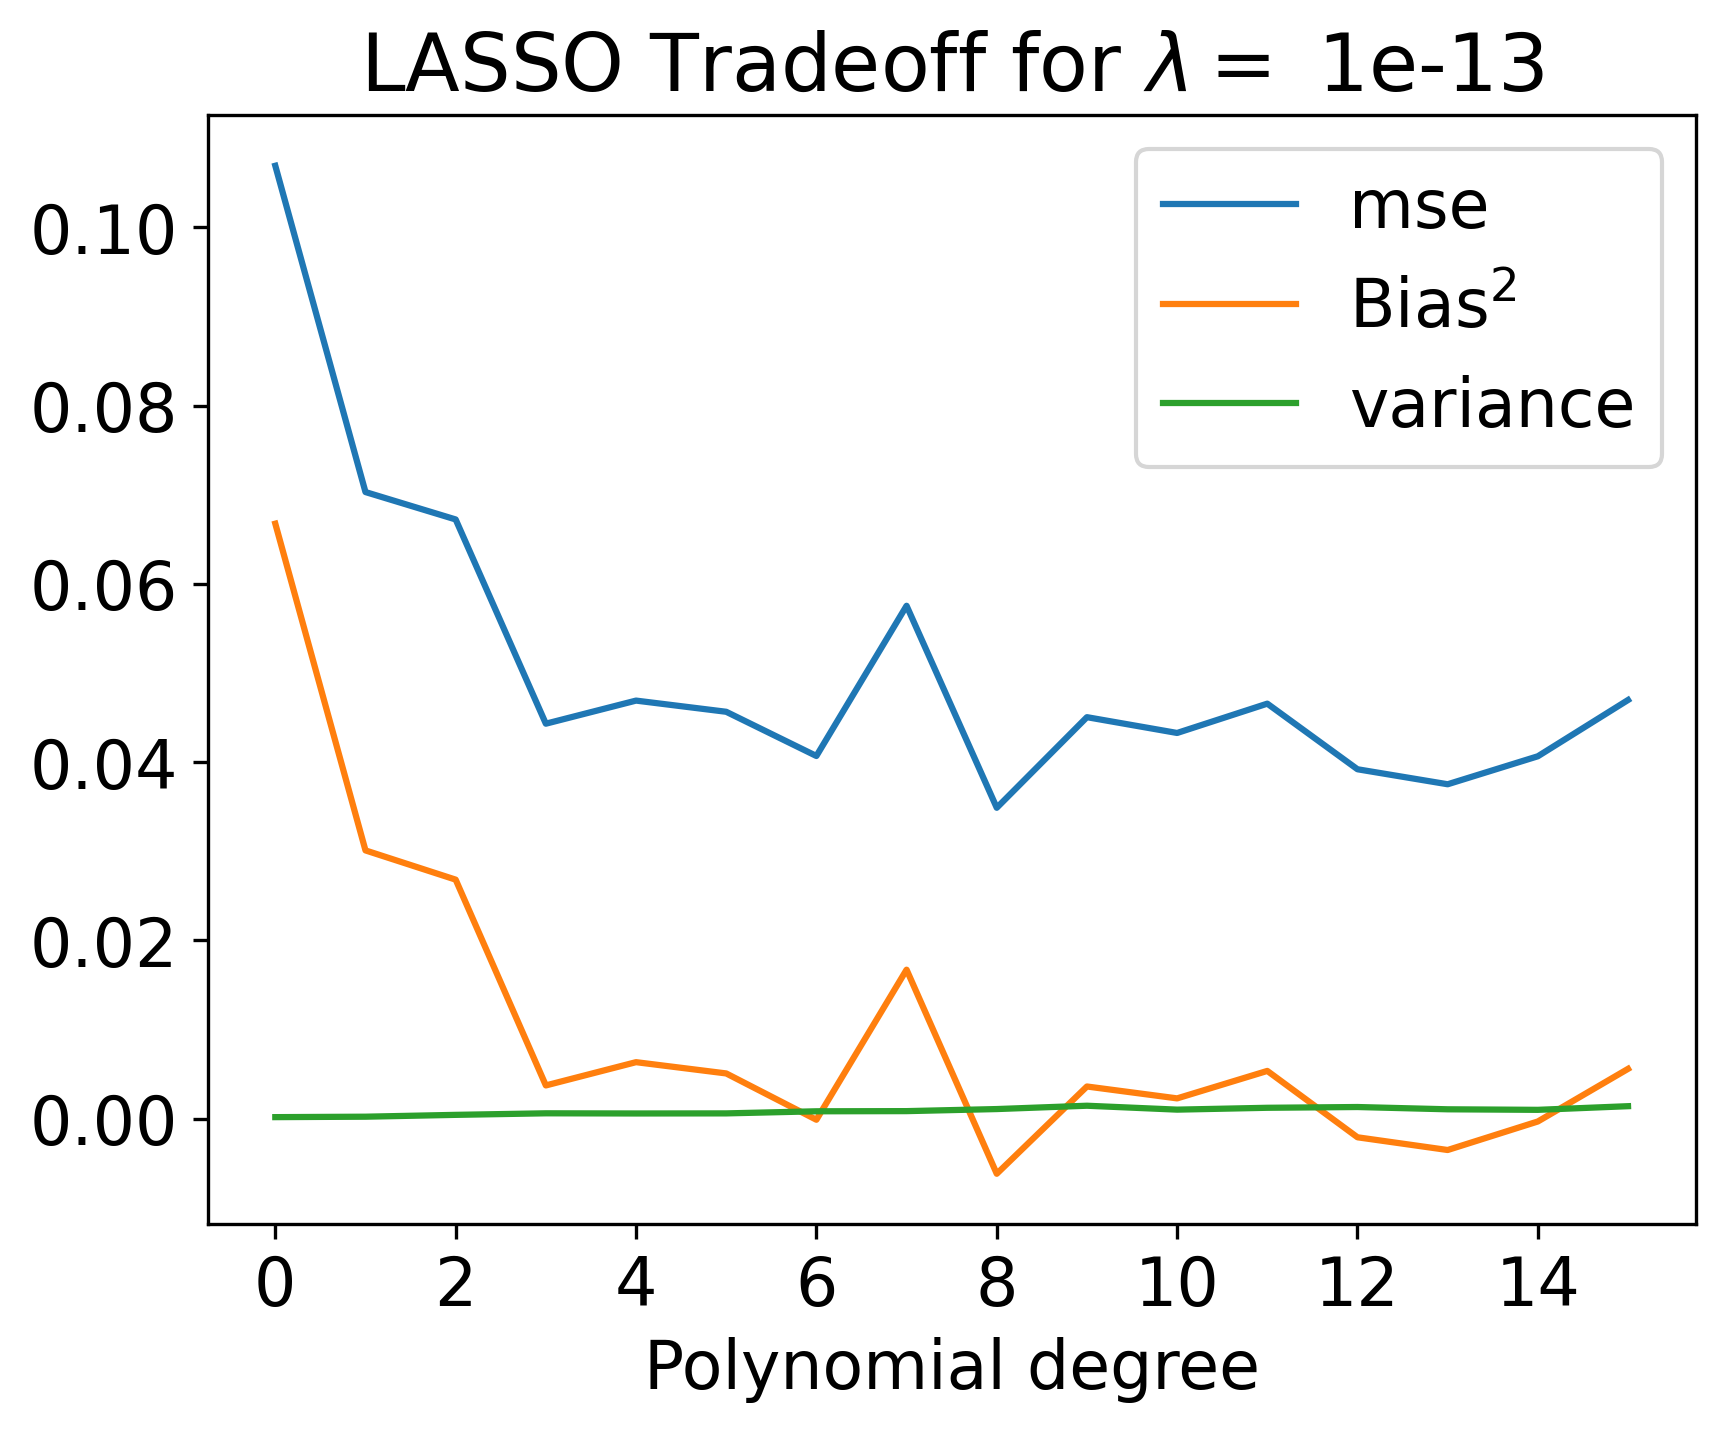
\includegraphics[width=\textwidth]{../figures/tradeoff_LASSO_1e-13.png}
    \caption{}
    \label{fig:l_1e-13}
  \end{subfigure}
  \caption{Bias variance tradeoff for different choices of lambda using Lasso regression for data with $n=30$ steps and noise standard deviation of $\sigma=0.2$}
  \label{fig:lasso_tradeoff}
\end{figure}
When comparing the two above figures (\ref{fig:ridge_tradeoff} and \ref{fig:lasso_tradeoff}) of the bias variance tradeoff with the tradeoff for OLS in figure \ref{fig:bias_variance} we see that ridge and lasso are much less prone to a fast increasing variance for higher degrees. It is also clear that the lasso regression is even better at keeping the variance down than the ridge regression even for smaller $\lambda$ parameters. It is in other words clear that the dampning parameter $\lambda$ does a great job of reducing overfiting for both ridge and lasso regression.

\subsubsection{Finding best models}
We continue with analyzing the error of our models dependency of polynomial degree and choice of the parameter $\lambda$. To best show this for lasso and ridge regression a heatmap is shown in figure \ref{fig:heat_franke} below where cross validation with 5 $k$-folds has been used. Here we have polynomial degree on the x-axis and $\lambda$ on the y-axis togethere with the MSE in color following the colorbar to the right of the figures.
\begin{figure}[H]

  \begin{subfigure}{.5\textwidth}
    \centering
    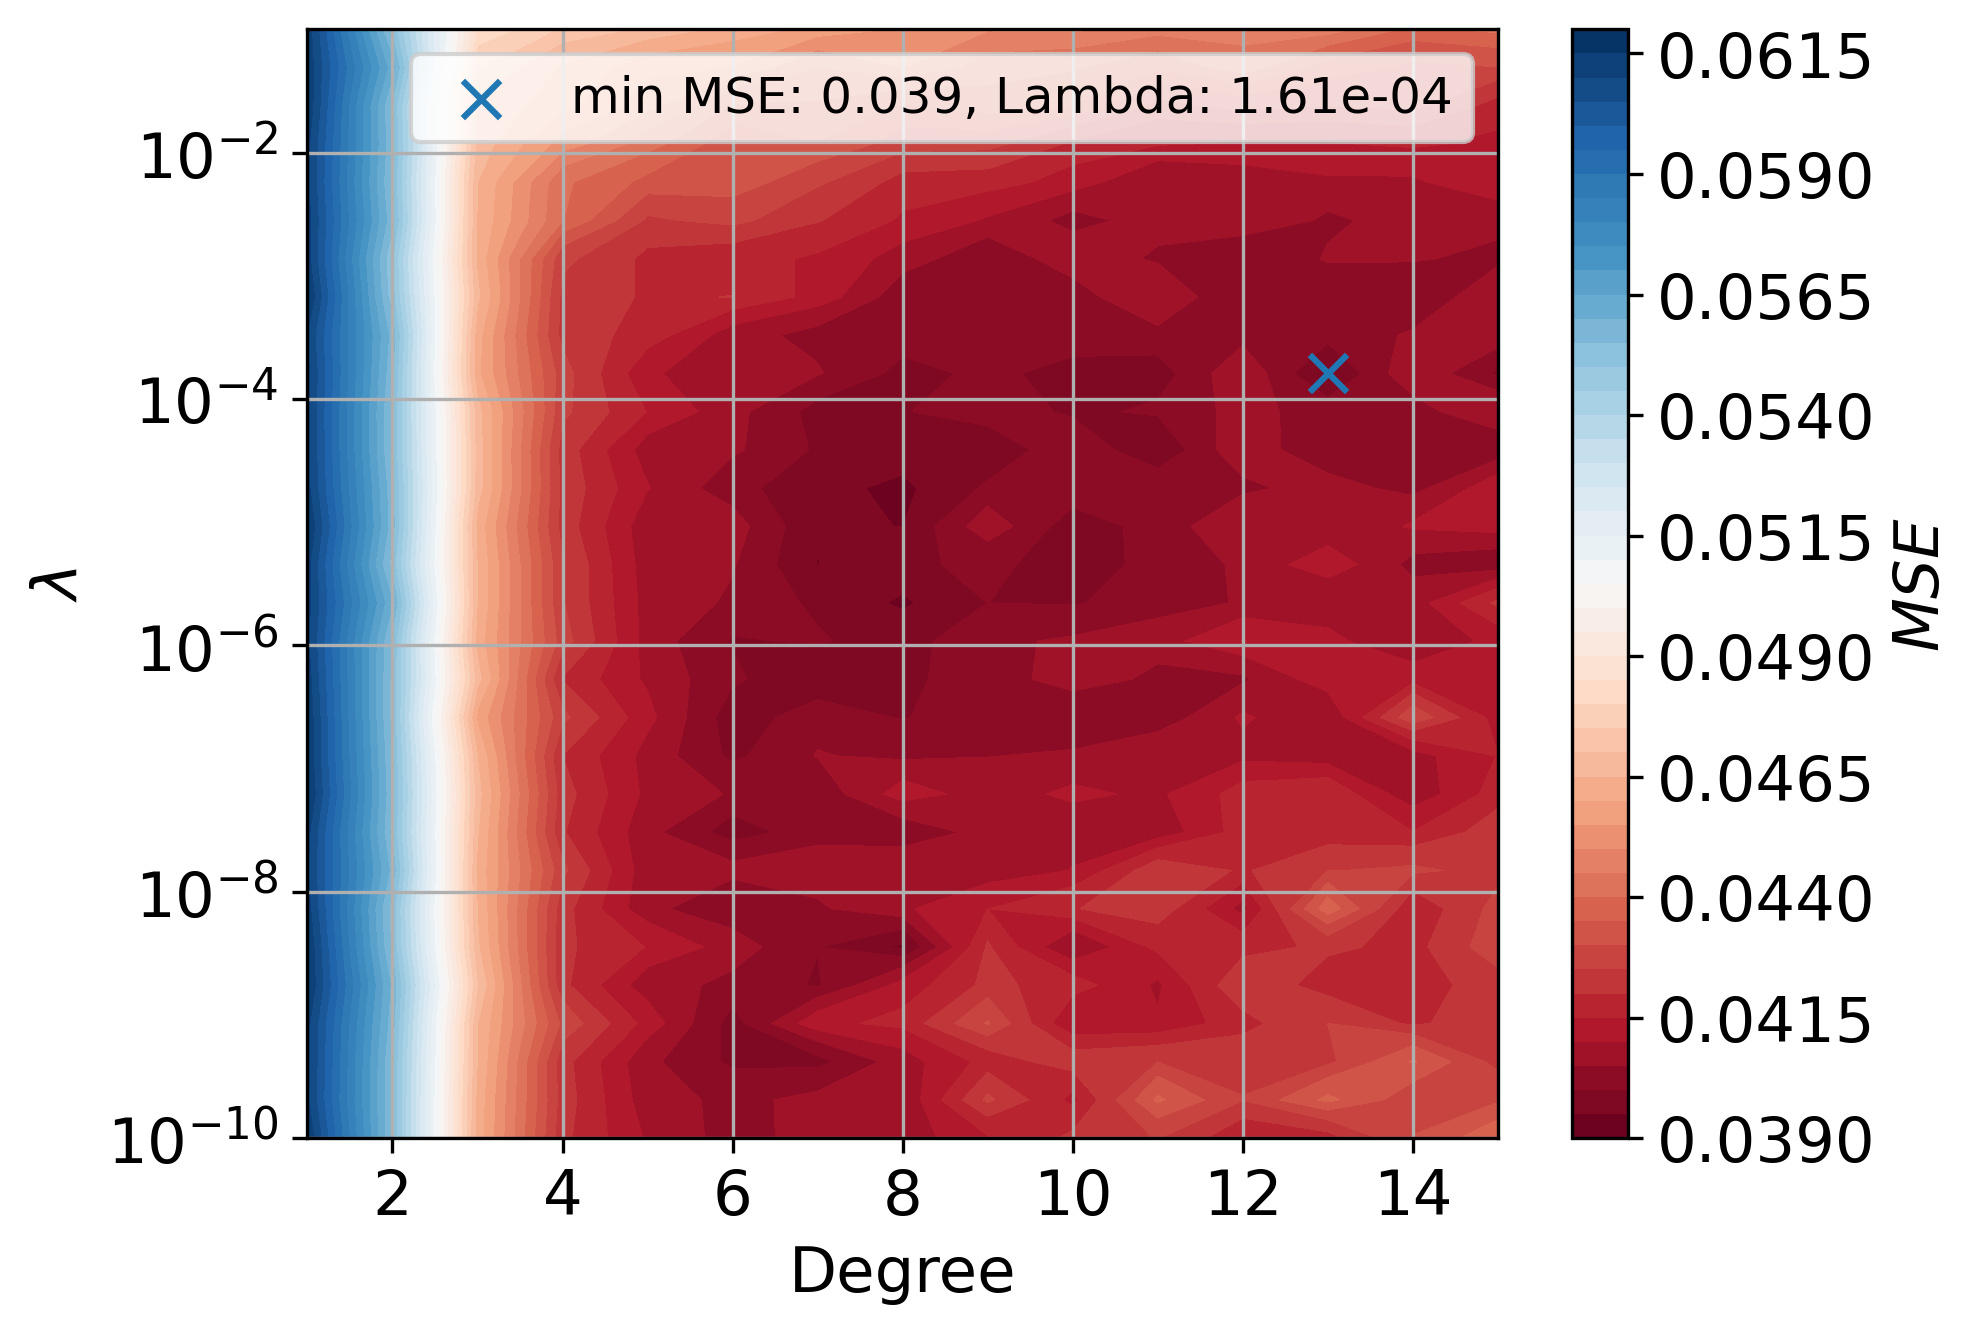
\includegraphics[width=\textwidth]{../figures/best_lambda_RIDGE_02.png}
    \caption{Ridge regression}
    \label{fig:}
  \end{subfigure}
  \begin{subfigure}{.5\textwidth}
    \centering
    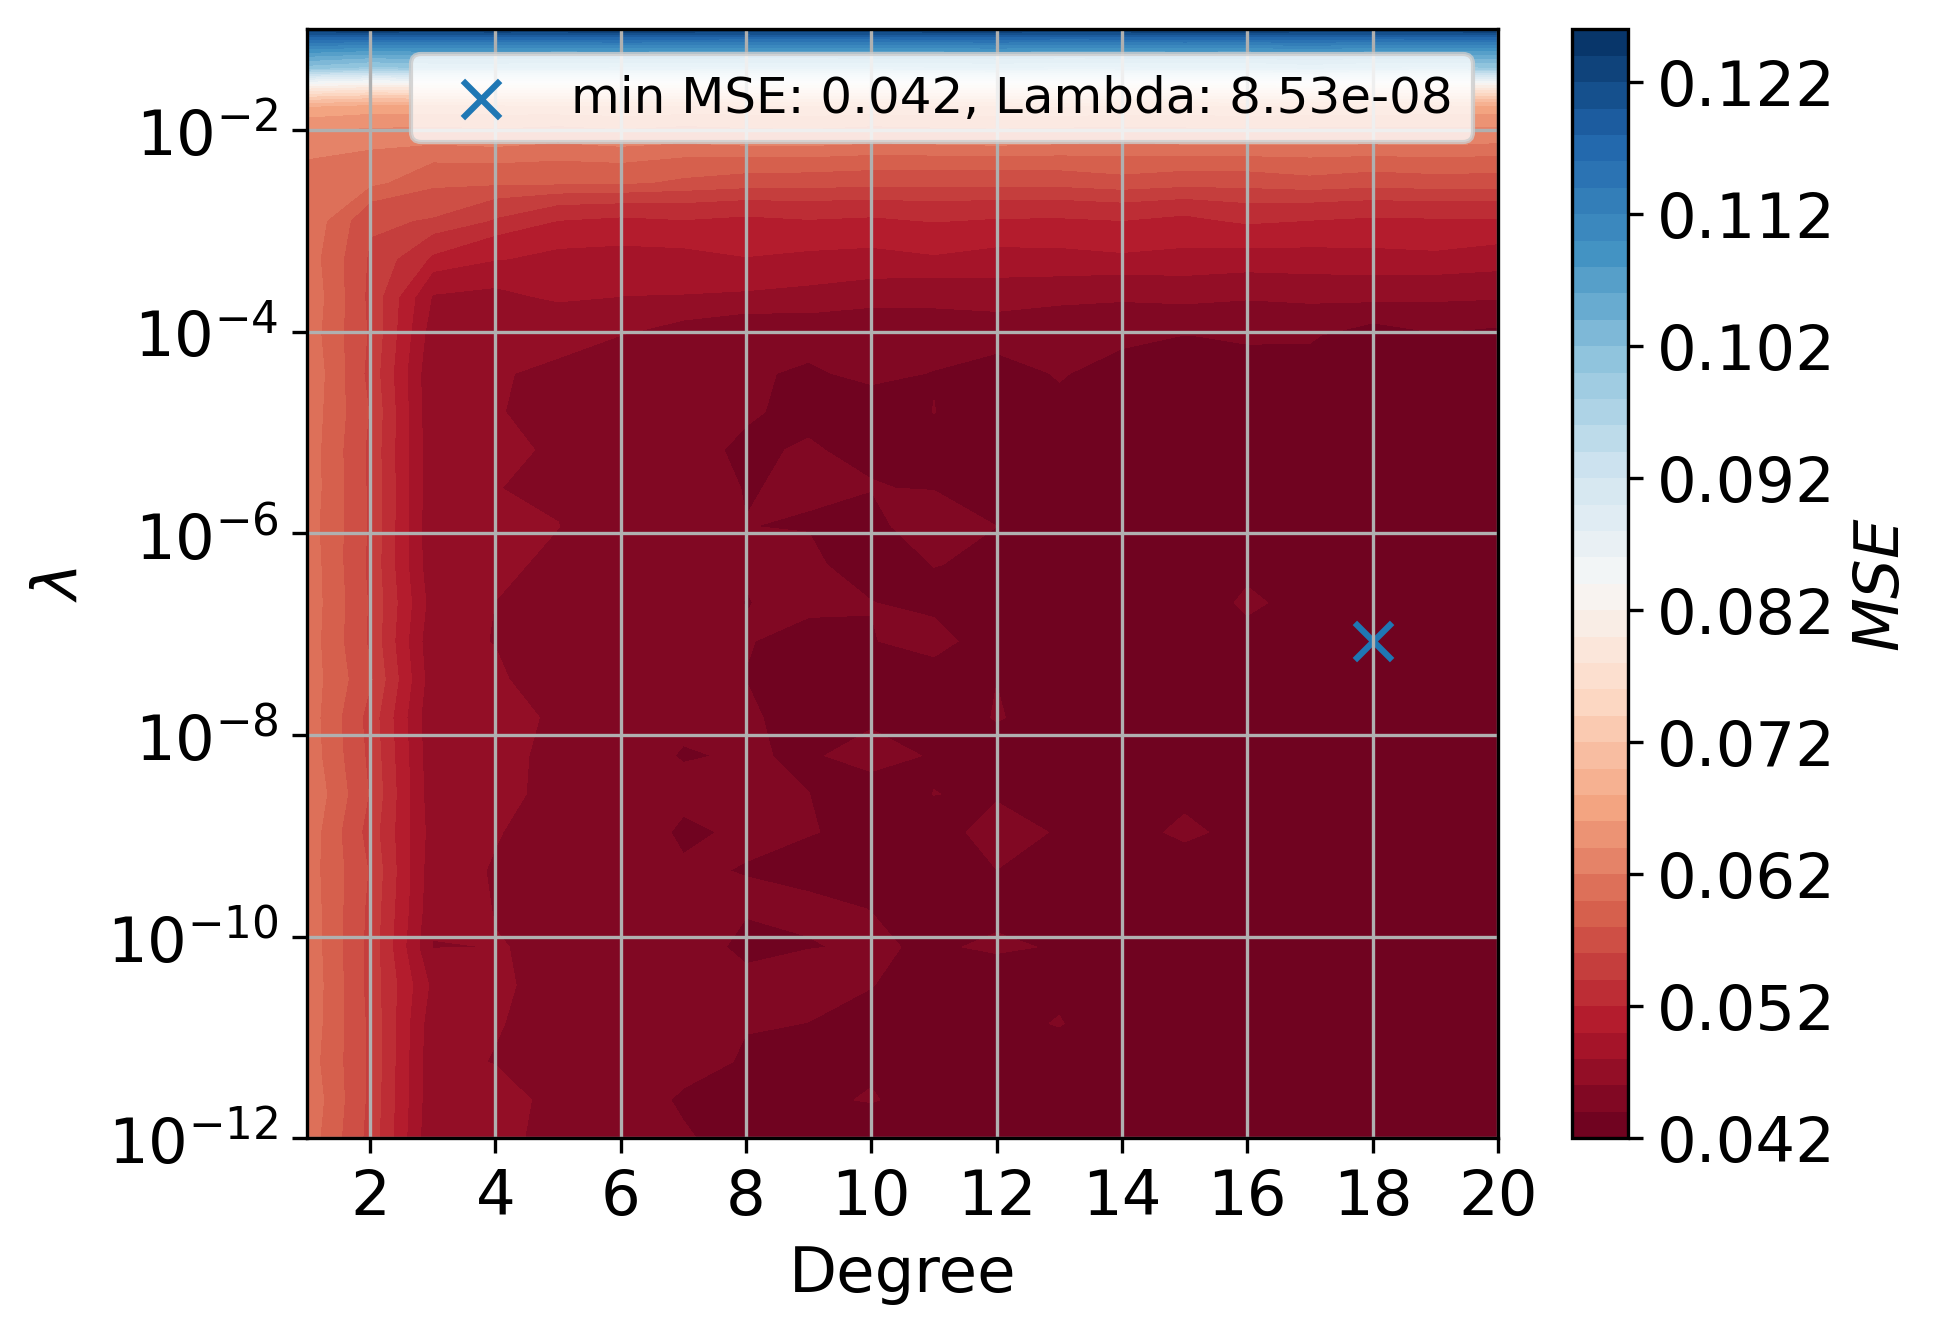
\includegraphics[width=\textwidth]{../figures/best_lambda_LASSO_02.png}
    \caption{Lasso regression}
    \label{fig:}
  \end{subfigure}
  \caption{Heatmap of MSE for different choices of polynomial degree and $\lambda$. Here we have used cross validation with 5$k$-folds for data with $n=30$ steps and noise standard deviation of $\sigma=0.2$}
  \label{fig:heat_franke}
\end{figure}
above in figure \ref{fig:heat_franke} we see a clear dependency of both $\lambda$ and polynomial degree for both ridge and lasso regression. Ridge aquires lower MSE for lower degrees than lasso which needs to be plotted up to a degree of 20 to finds an optimal degree of 18. MSE in the ridge plot is variating more when changing $\lambda$ than what we see for the lasso method. This corresponds to what we saw in the bias variance tradeoff in figure \ref{fig:ridge_tradeoff} and \ref{fig:lasso_tradeoff} where we saw almost no change for the lasso tradeoff for a changing $\lambda$. This together with figure \ref{fig:best_OLS} have given us a way of finding which model gives the most optimal results. This is shown in table \ref{tab:best_comp}.
\begin{table}
  \centering
  \caption{Table of best parameters and the following MSE for OLS, Ridge and Lasso regression}
  \label{tab:best_comp}
  \begin{tabular}{|c||c|c|c|}
    \hline
    Method & $\lambda$ & Degree & $MSE$ \\
    \hline
    OLS &  & 6 & 0.0393 \\
    \hline
    RIDGE & $3.04\times10^{-8}$ & 6 & 0.0394 \\
    \hline
    LASSO & $8.53\times10^{-8}$ & 18 & 0.042 \\
    \hline
  \end{tabular}
\end{table}
We see from table \ref{tab:best_comp} very close results, espceially between OLS and Ridge regression. OLS beats Ridge with a slightly lower MSE while Lasso is still a bit behind them both.
\subsubsection{Prediction plots}
We use the results from table \ref{tab:best_comp} to show the predictions of our models in figure \ref{fig:pred_franke} below.
\begin{figure}[H]
  \begin{subfigure}{.5\textwidth}
    \centering
    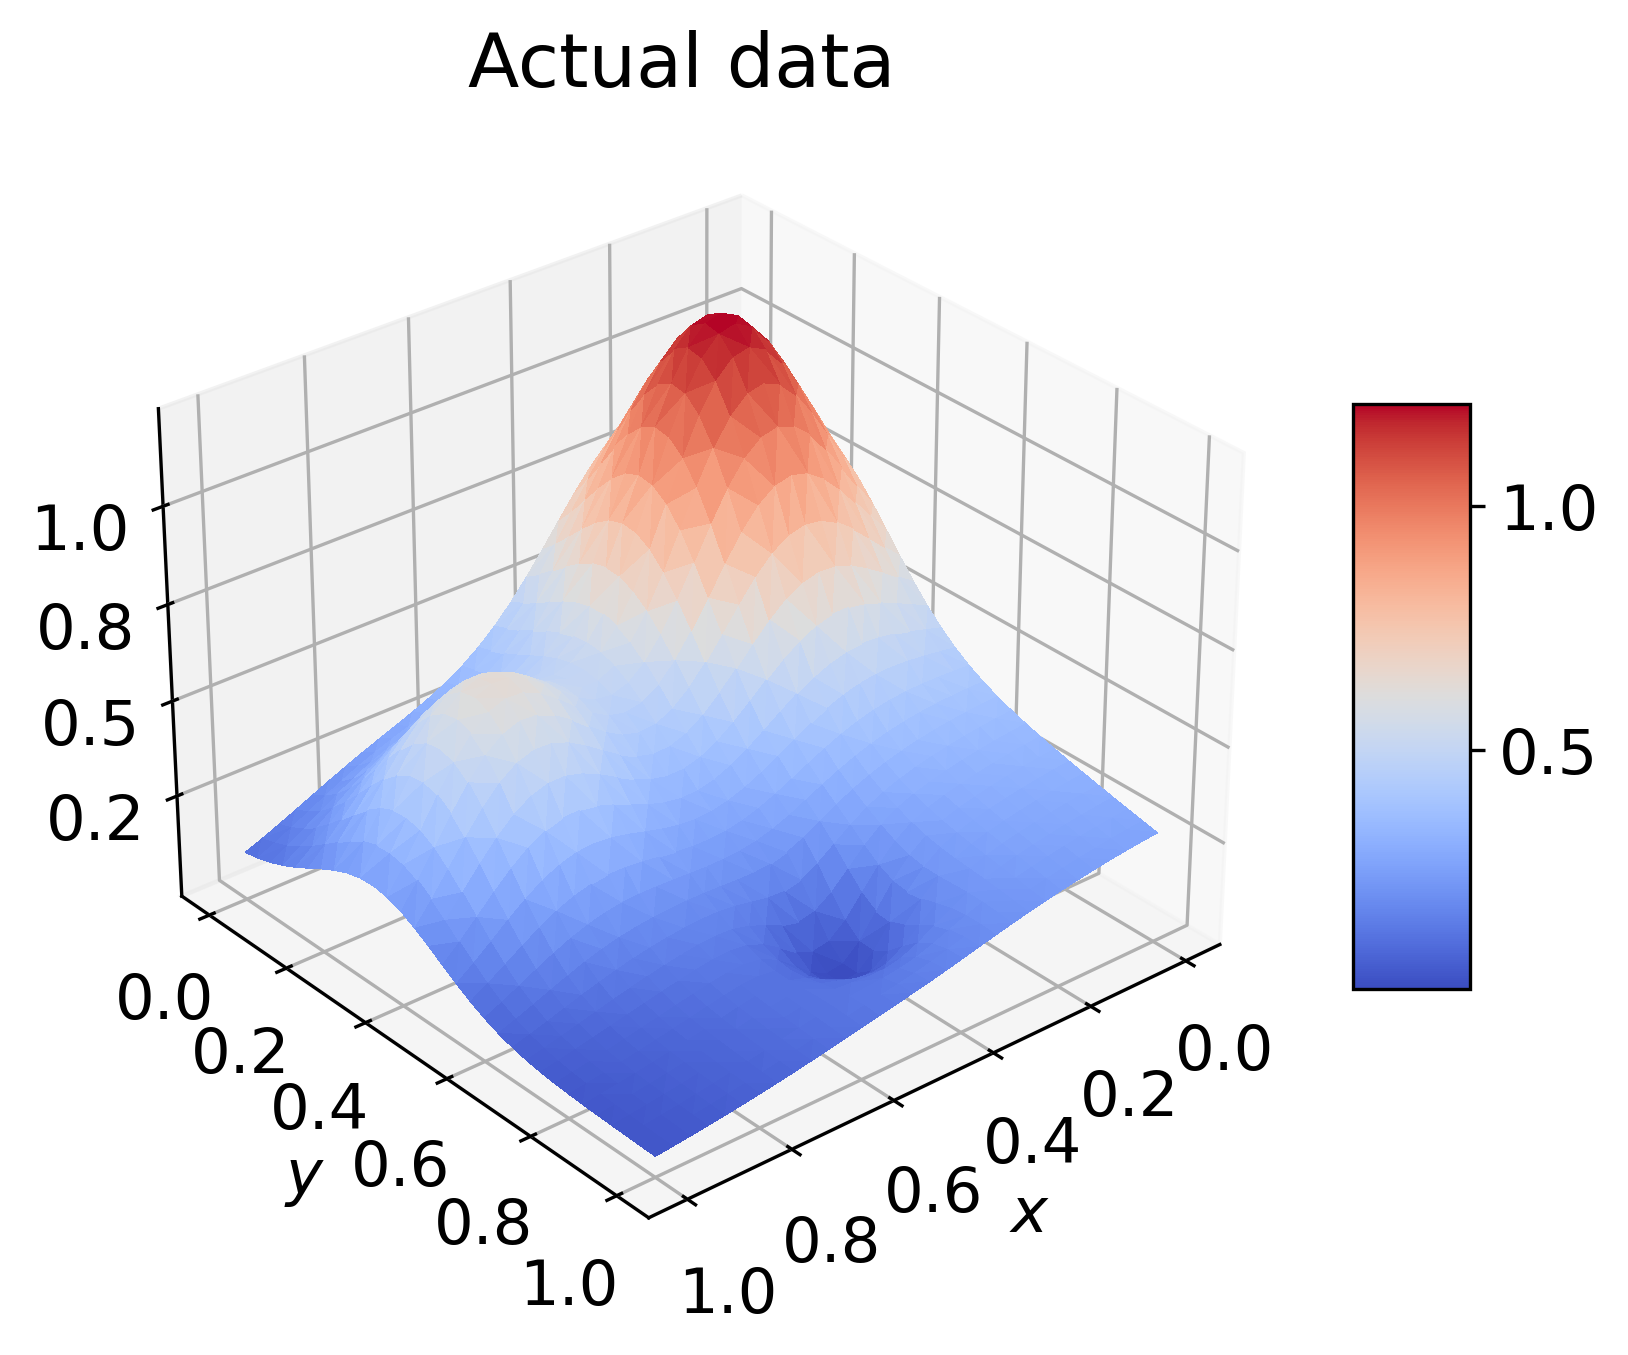
\includegraphics[width=\textwidth]{../figures/actual_data_franke_2.png}
    \caption{Franke function}
    \label{fig:pred_real}
  \end{subfigure}
  \begin{subfigure}{.5\textwidth}
    \centering
    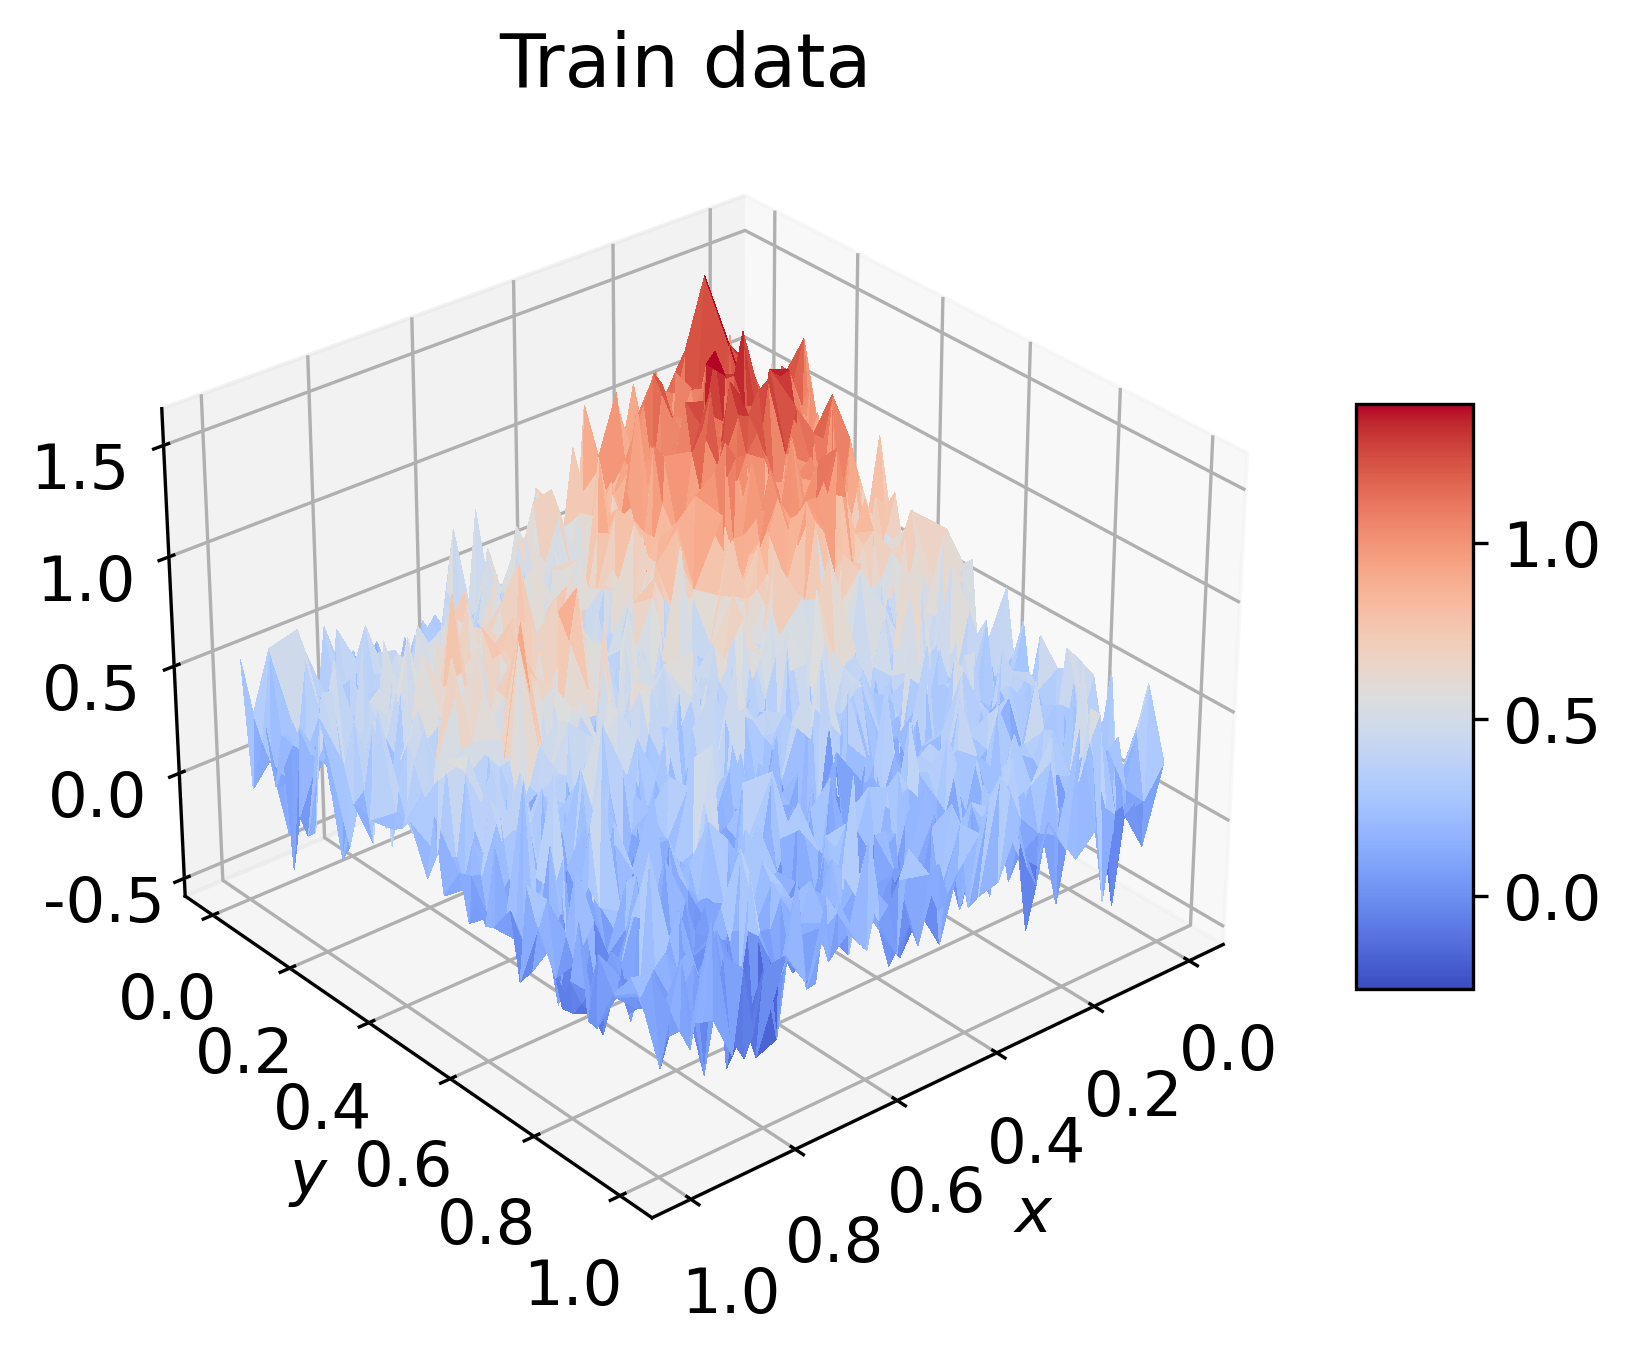
\includegraphics[width=\textwidth]{../figures/train_data_franke_2.png}
    \caption{Train data from function data with added noise}
    \label{fig:pred_train}
  \end{subfigure}
  \begin{subfigure}{.5\textwidth}
    \centering
    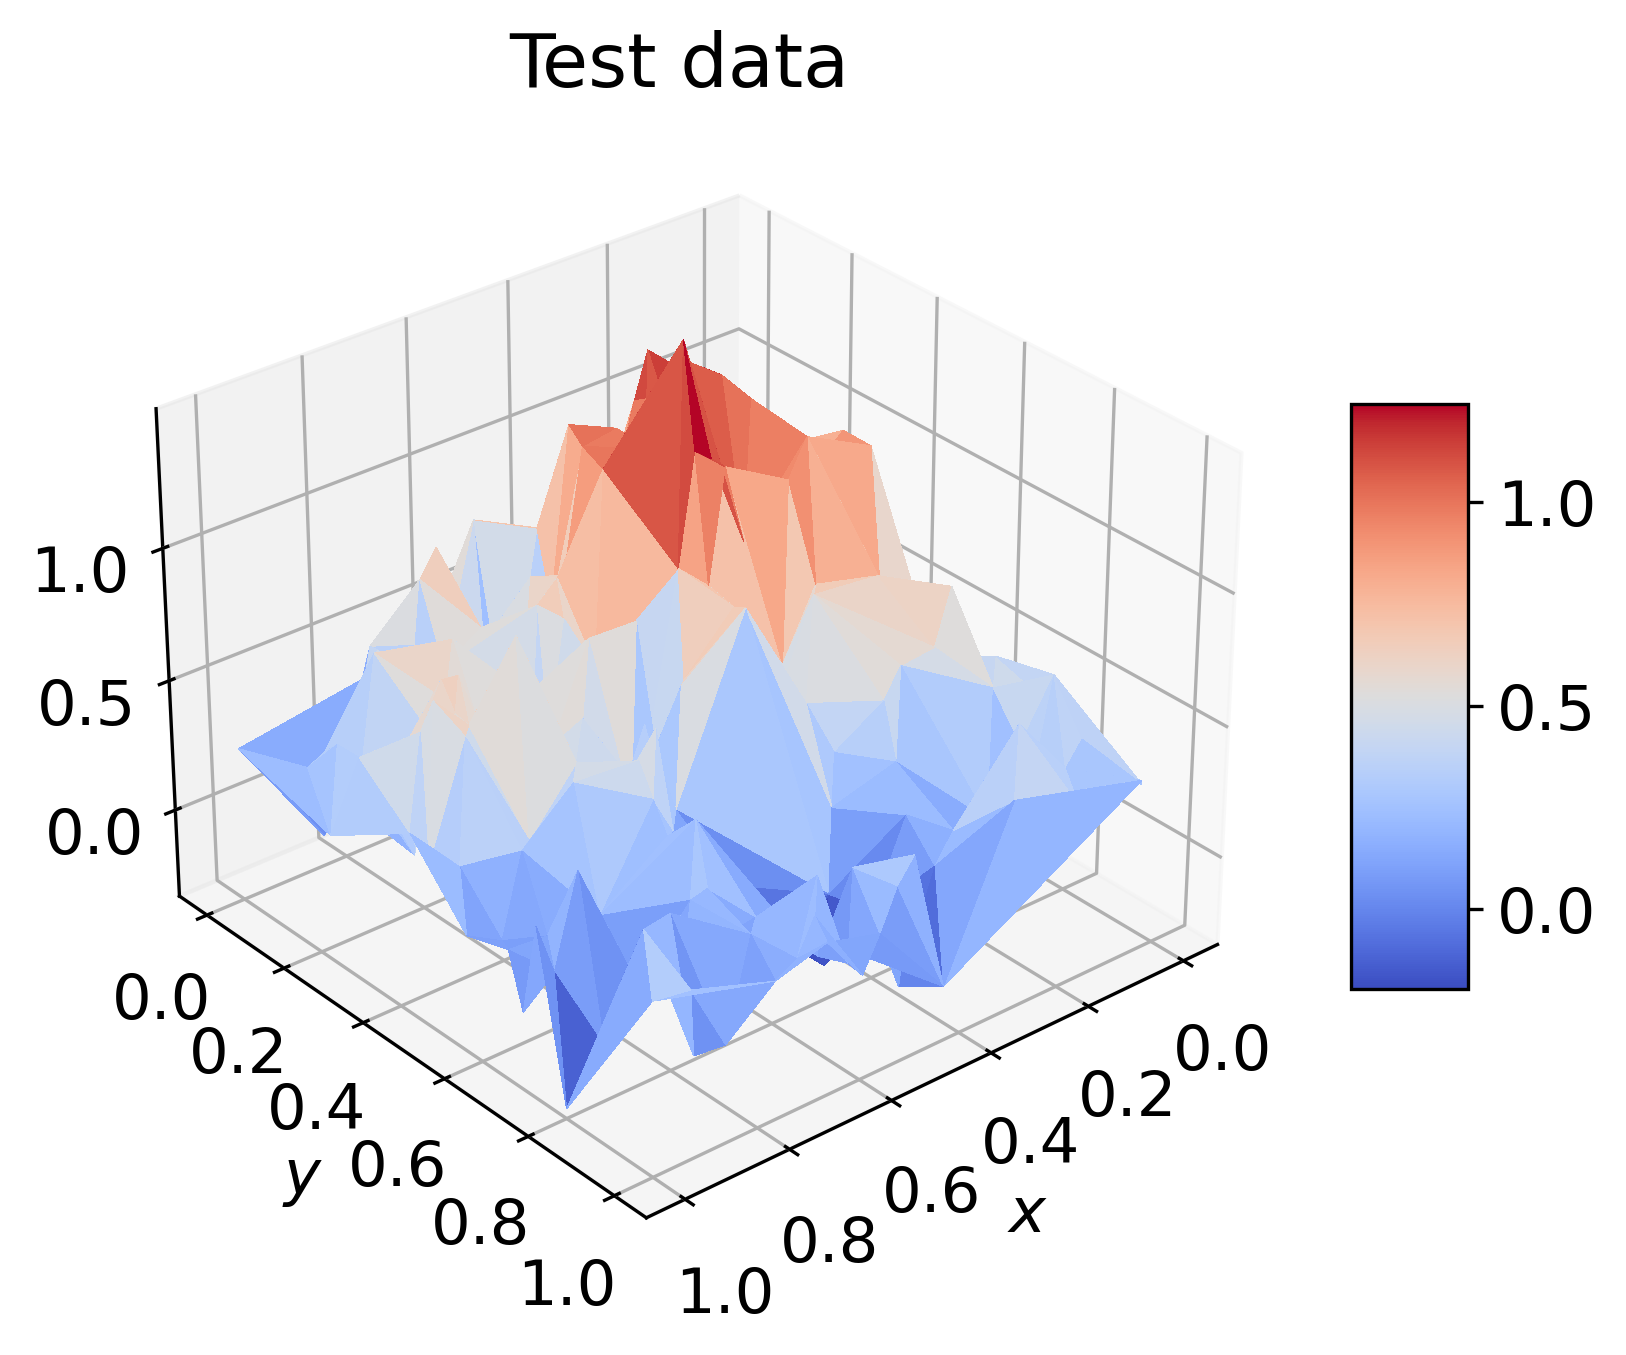
\includegraphics[width=\textwidth]{../figures/test_data_franke_2.png}
    \caption{Test data from function data with added noise}
    \label{fig:pred_test}
  \end{subfigure}
  \begin{subfigure}{.5\textwidth}
    \centering
    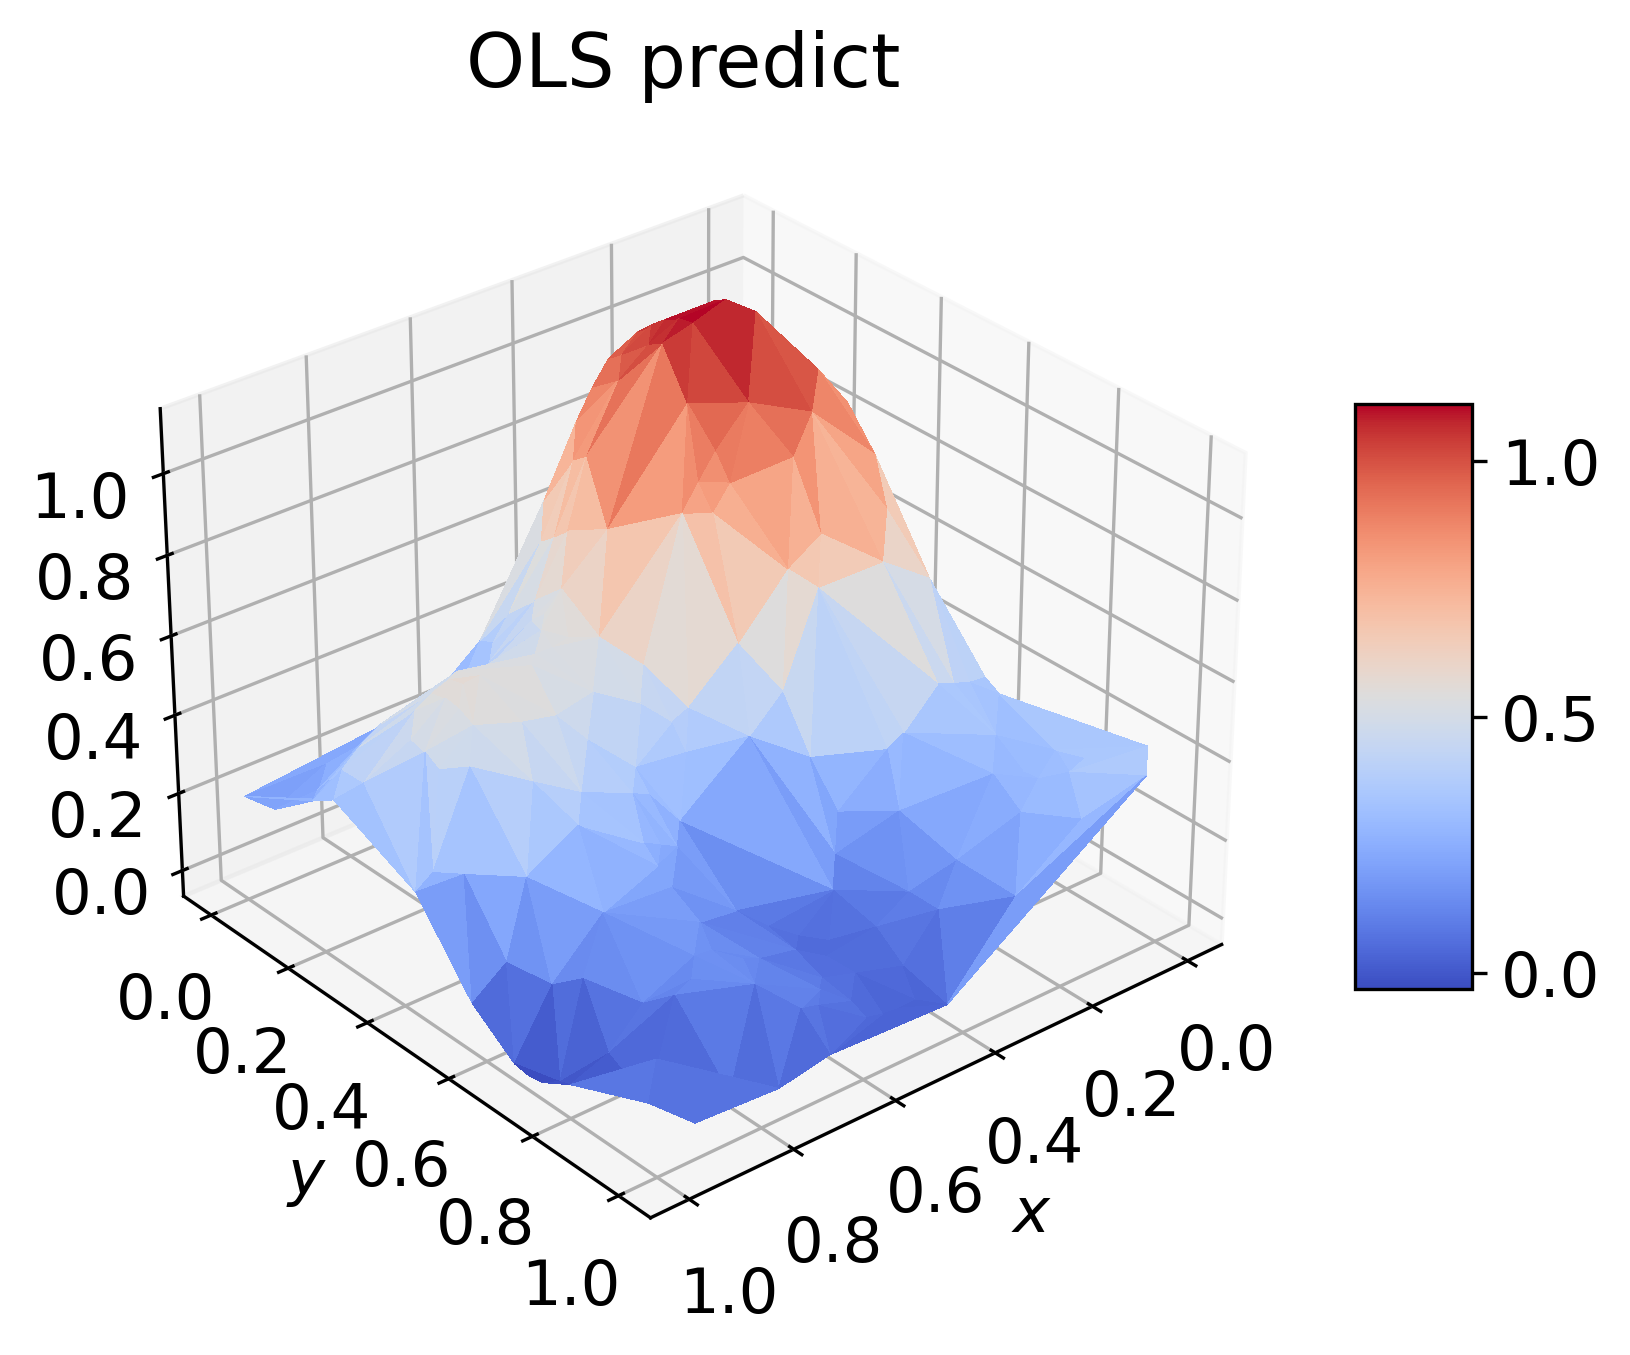
\includegraphics[width=\textwidth]{../figures/ols_pred_franke_2.png}
    \caption{OLS prediction}
    \label{fig:pred_ols}
  \end{subfigure}
  \begin{subfigure}{.5\textwidth}
    \centering
    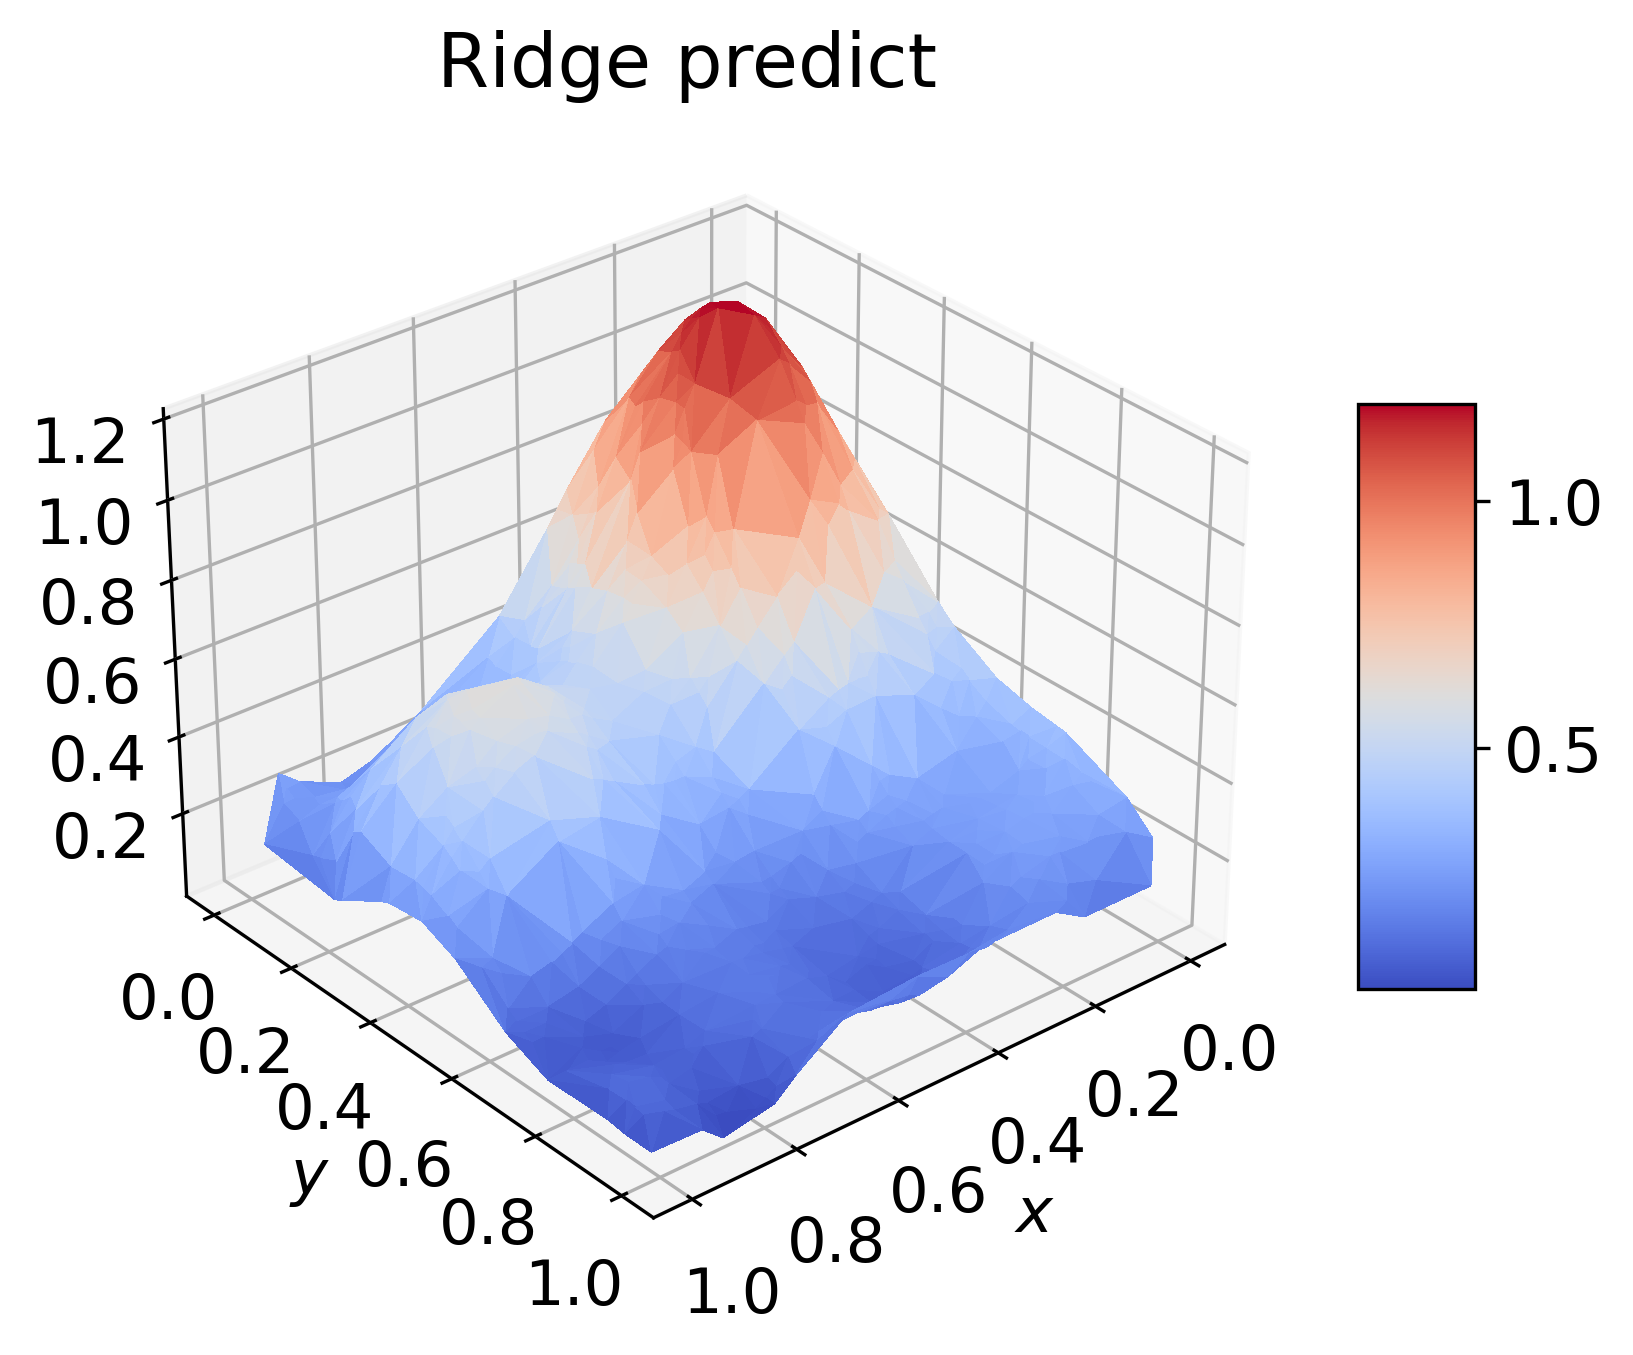
\includegraphics[width=\textwidth]{../figures/ridge_pred_franke_2.png}
    \caption{Ridge prediction}
    \label{fig:pred_ridge}
  \end{subfigure}
  \begin{subfigure}{.5\textwidth}
    \centering
    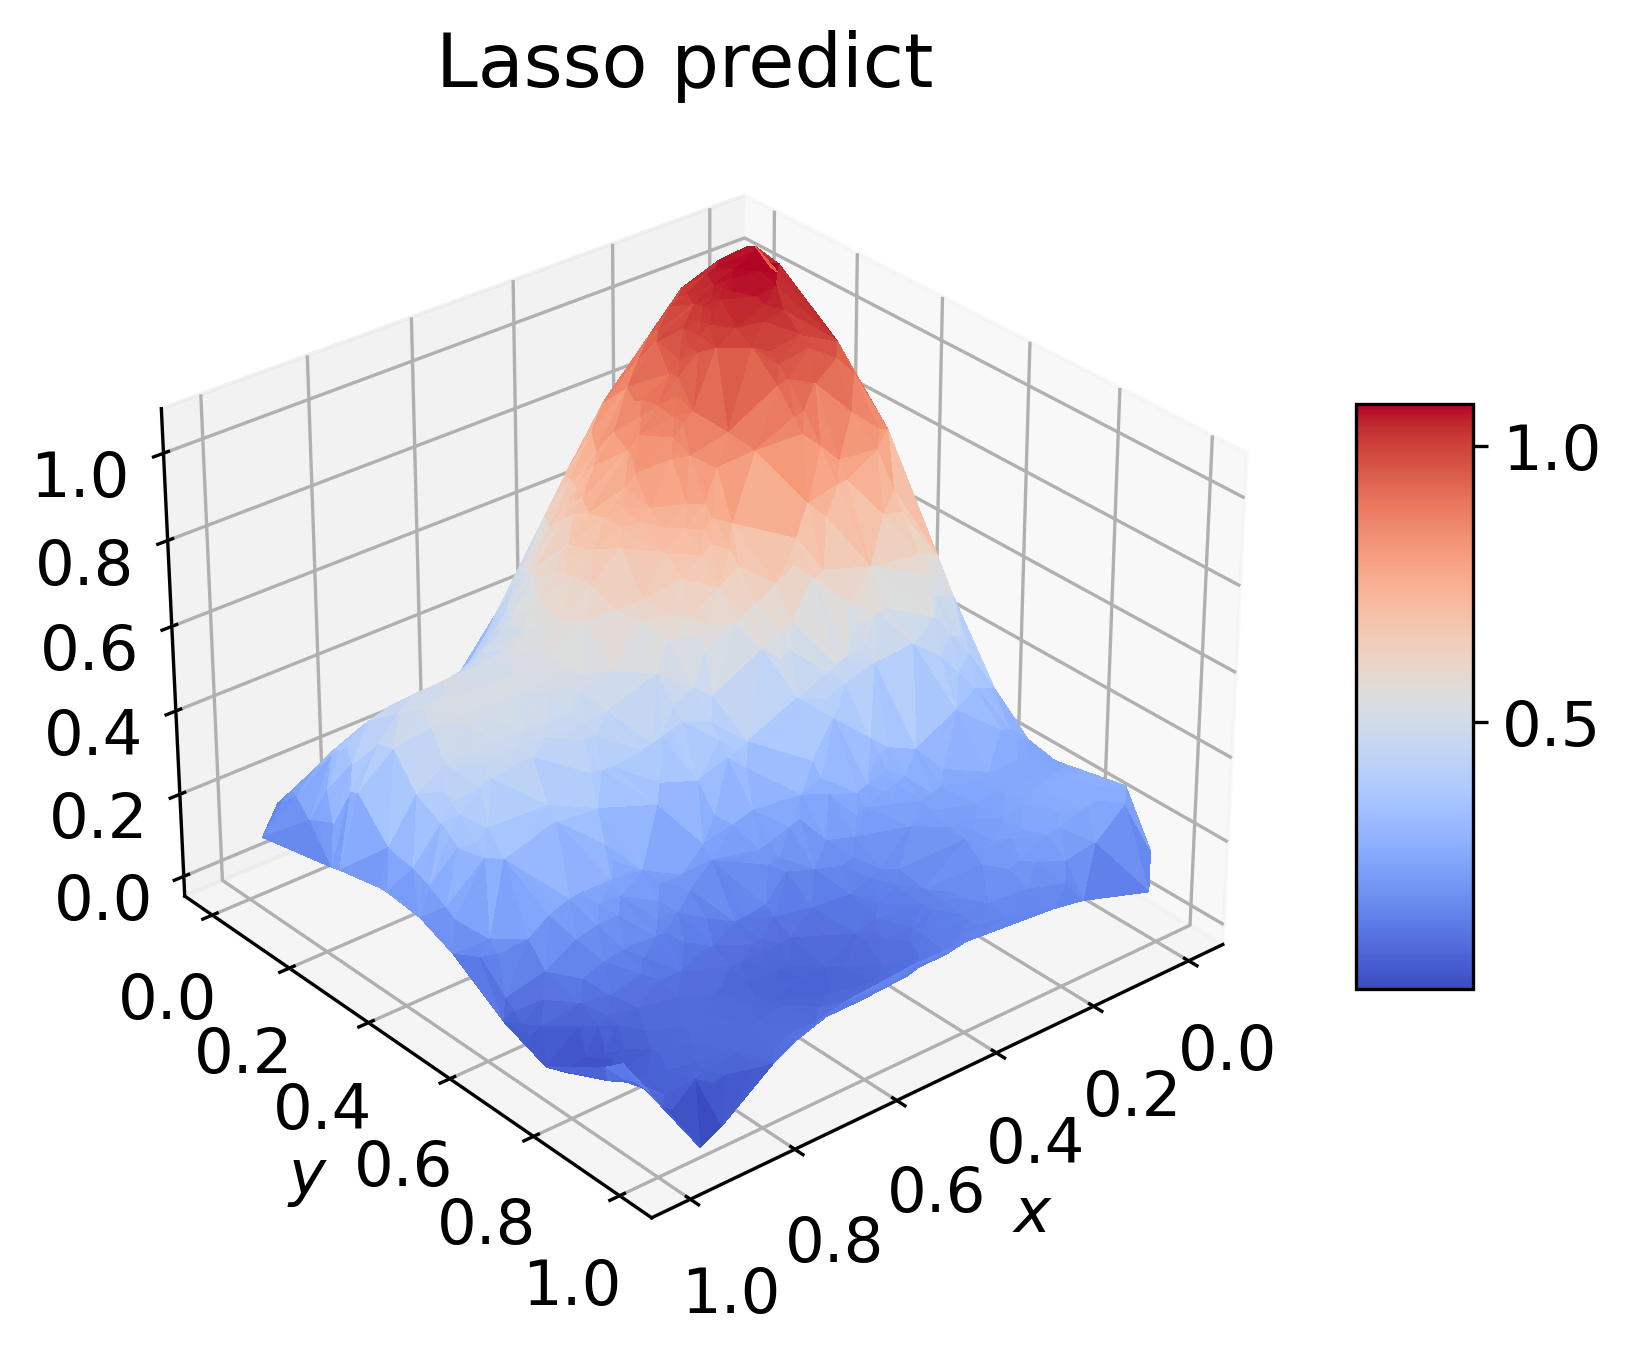
\includegraphics[width=\textwidth]{../figures/lasso_pred_franke_2.png}
    \caption{Lasso prediction}
    \label{fig:pred_lasso}
  \end{subfigure}
  \caption{Plot of the true Franke function together with our train and test data, and our predictions for our optimal parameters shown in table \ref{tab:best_comp} }
  \label{fig:pred_franke}
\end{figure}
We see that our predictions follow the general trend of the franke function shown in figure \ref{fig:pred_real}. We see small differences between the 3 different predictions \ref{fig:pred_ols}, \ref{fig:pred_ridge}, and \ref{fig:pred_lasso}, but it remains hard to tell which does the best prediction without looking at table \ref{tab:best_comp}. Our plots are also quite choppy as a result of the small test sample. Here we have again used $n=30$ steps and a standard deviation of $\sigma=0.2$ which leaves us with an even smaller test sample and following resuoulution in our prediction plots.
\subsection{Topography data}
We now look at real topography data and begin seeing how our predictions react to design matrices of different plynomial degree. We see in figure \ref{fig:mse_r2_real}
\begin{figure}[H]
  \begin{subfigure}{.5\textwidth}
    \centering
    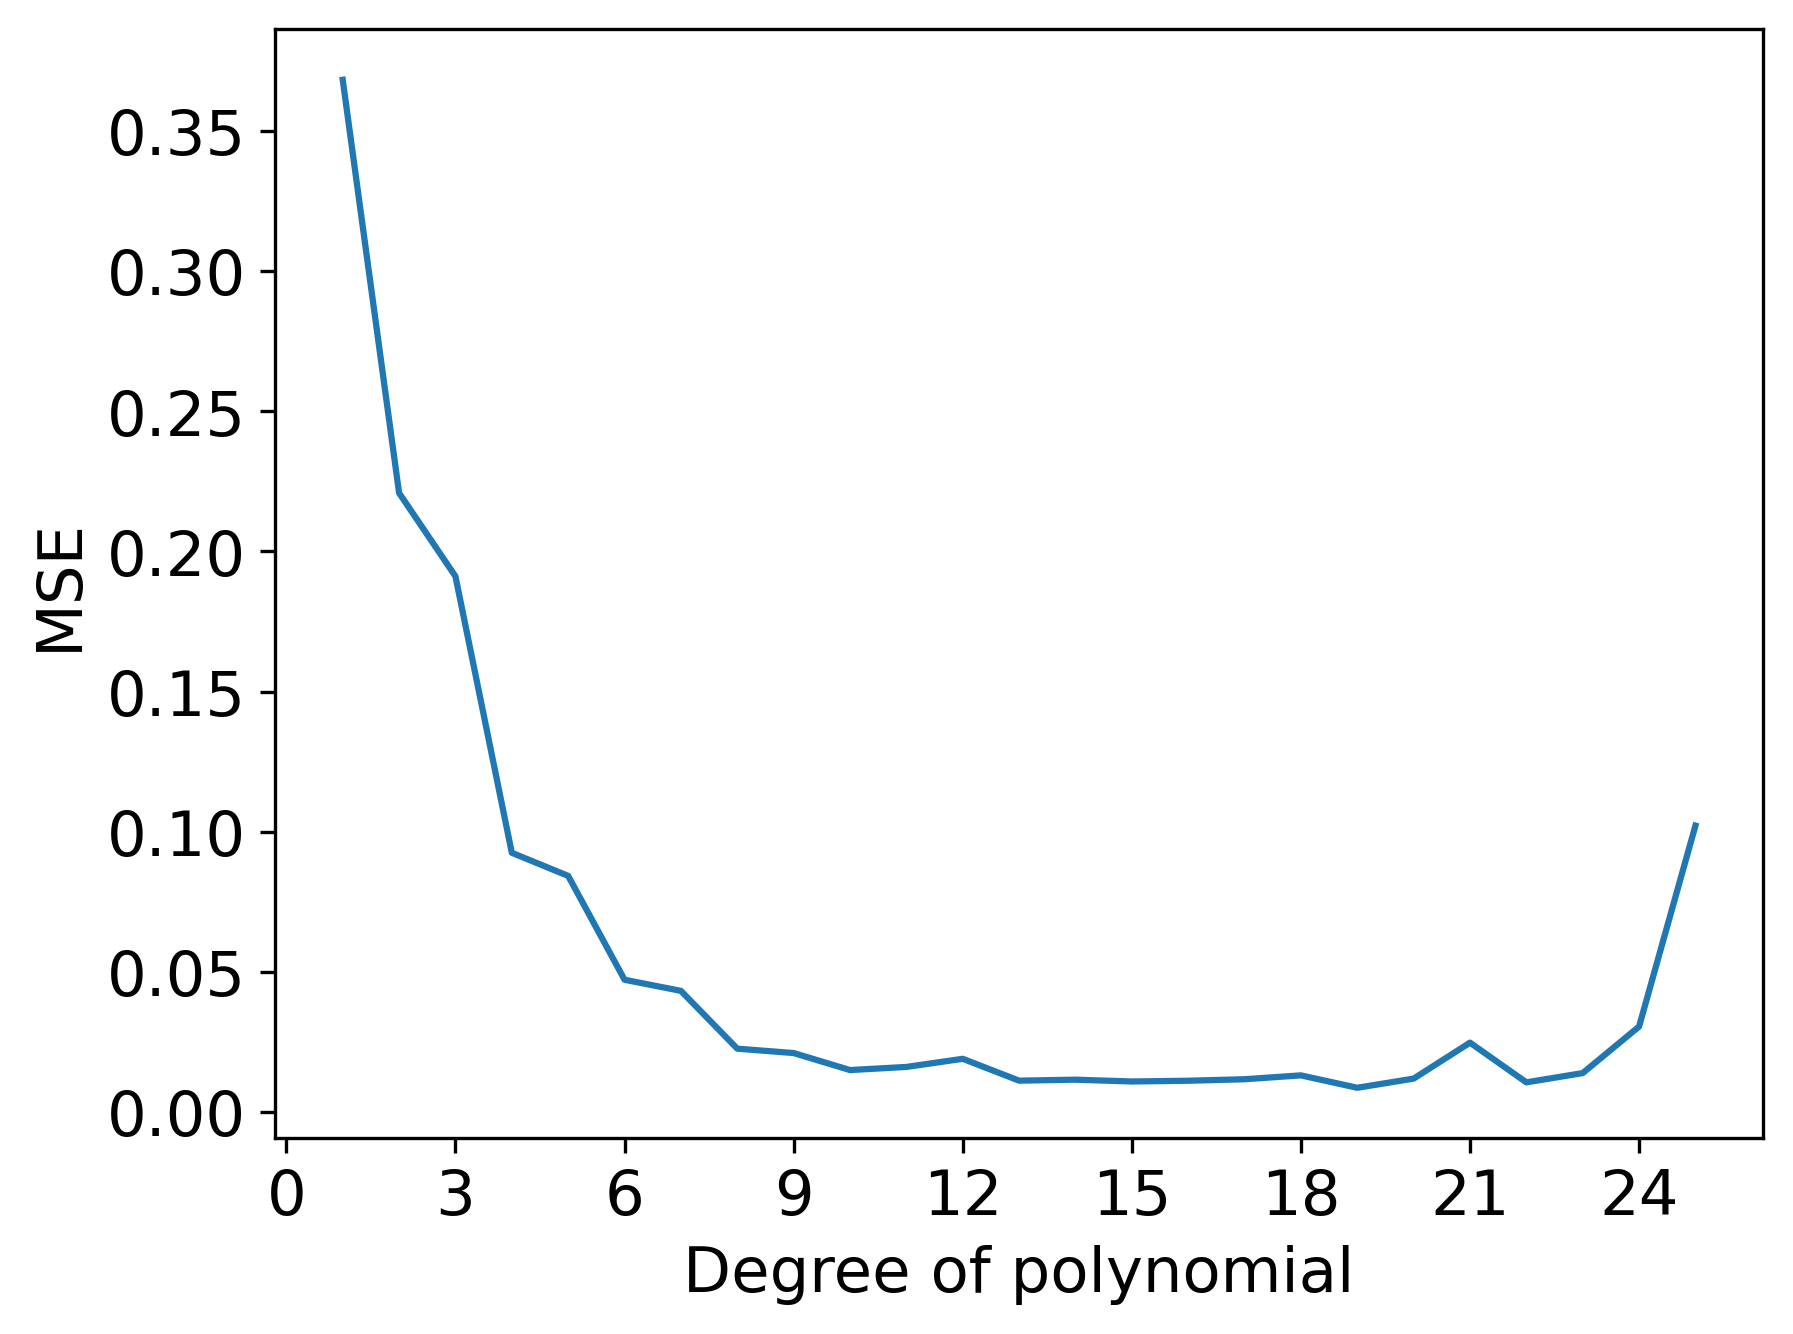
\includegraphics[width=\textwidth]{../figures/mse_deg_real.png}
    \caption{}
    \label{fig:}
  \end{subfigure}
  \begin{subfigure}{.5\textwidth}
    \centering
    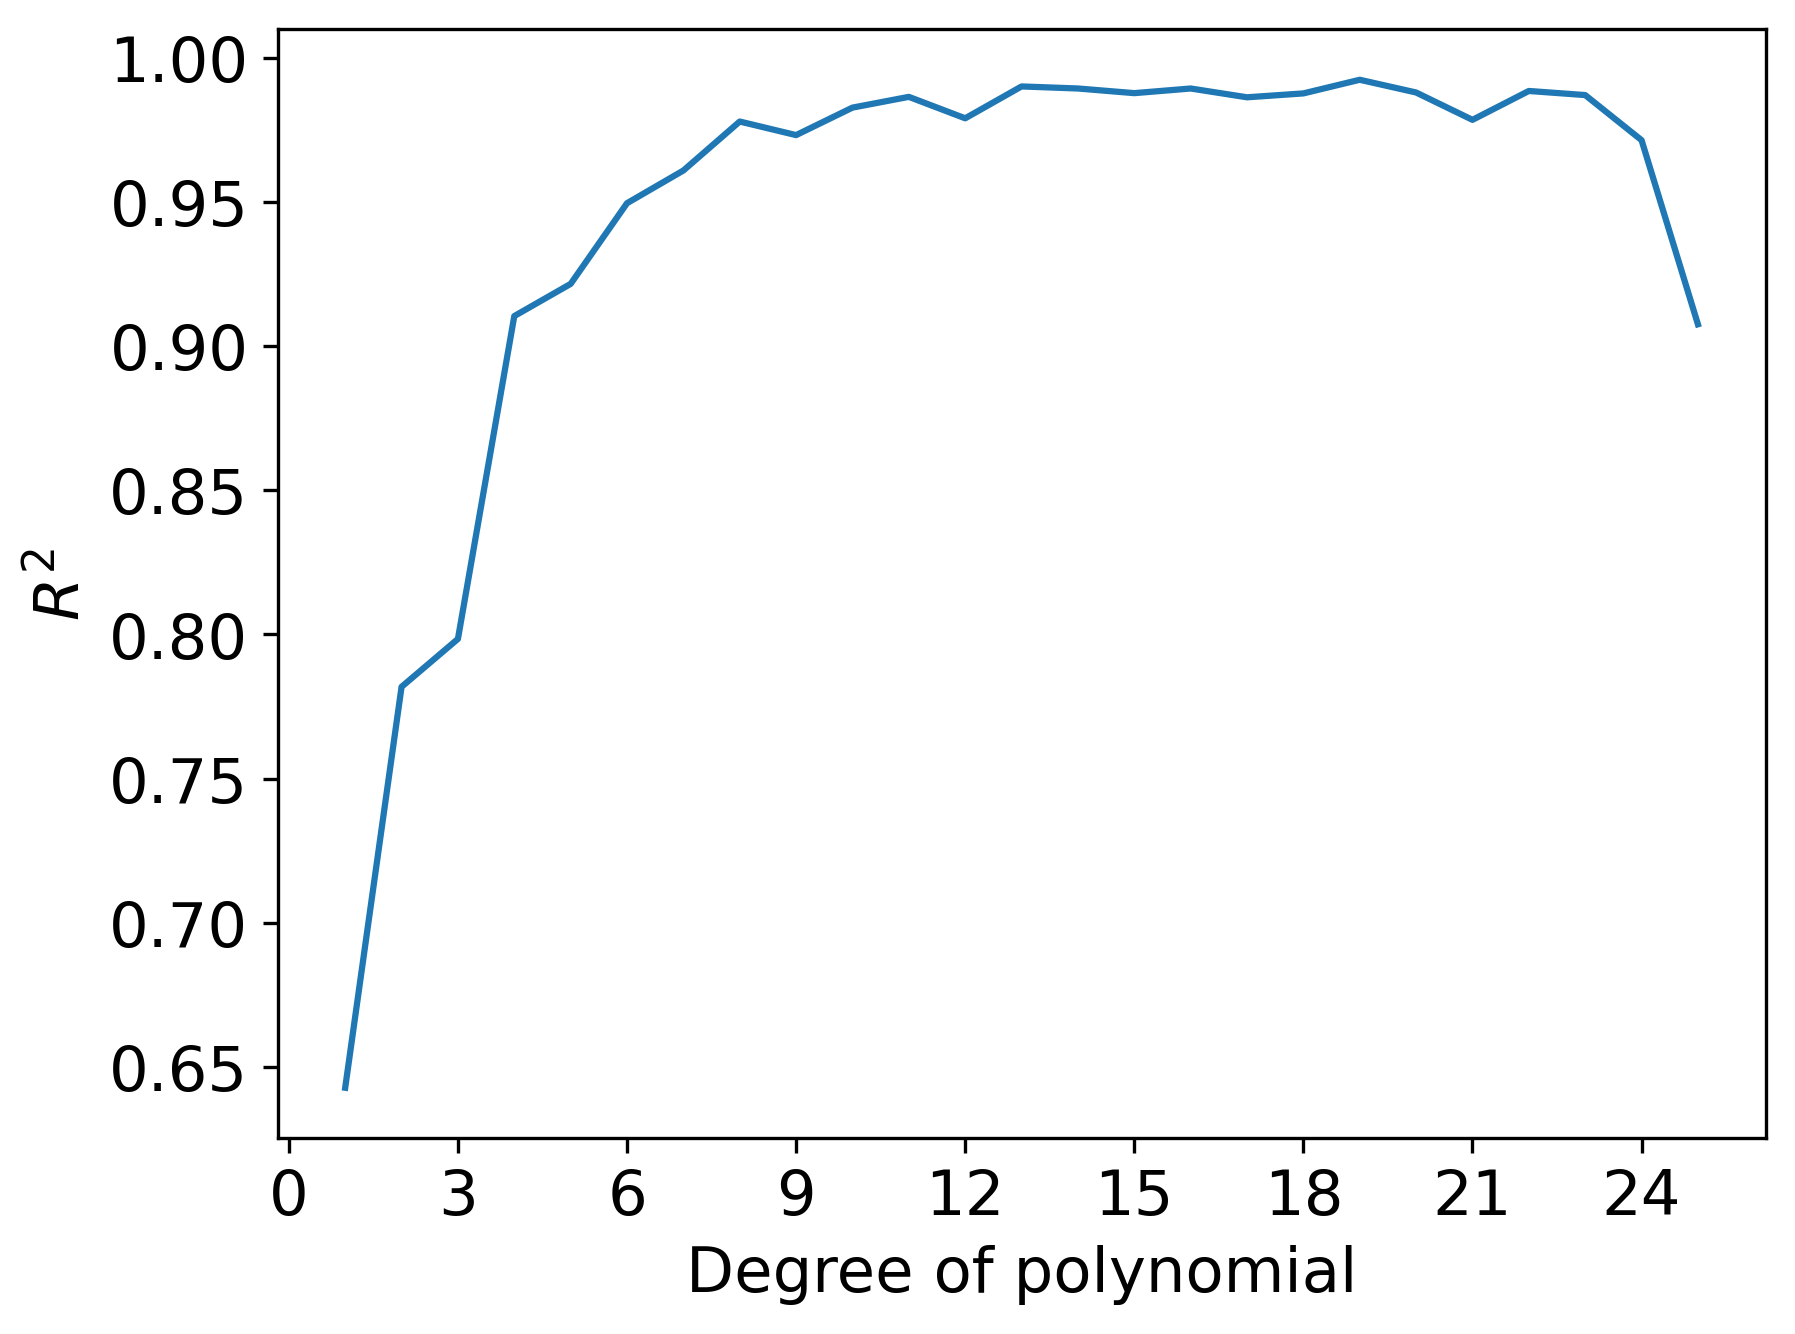
\includegraphics[width=\textwidth]{../figures/r2_deg_real.png}
    \caption{}
    \label{fig:}
  \end{subfigure}
  \caption{MSE and $R^2$ as a function of polynomial degree for OLS predction. Here we are using indexes of [100:141] where every second index are skipped.}
  \label{fig:mse_r2_real}
\end{figure}
We see what seems like overfitting happining around a degree of 22 which is alot higher than what we saw for the franke function. This indicates that we need a more advanced function to describe our data.

\subsubsection{Bias variance tradeoff}
We perform the bias variance tradeoff for the three methods for a degree up to 25, and for ridge and lasso also different $\lambda$ parameters. OLS in figure \ref{fig:tradeoff_real}, Ridge in figure \ref{fig:ridge_tradeoff_real} and Lasso in figure \ref{fig:lasso_tradeoff_real}
\begin{figure}[H]
  \centering
  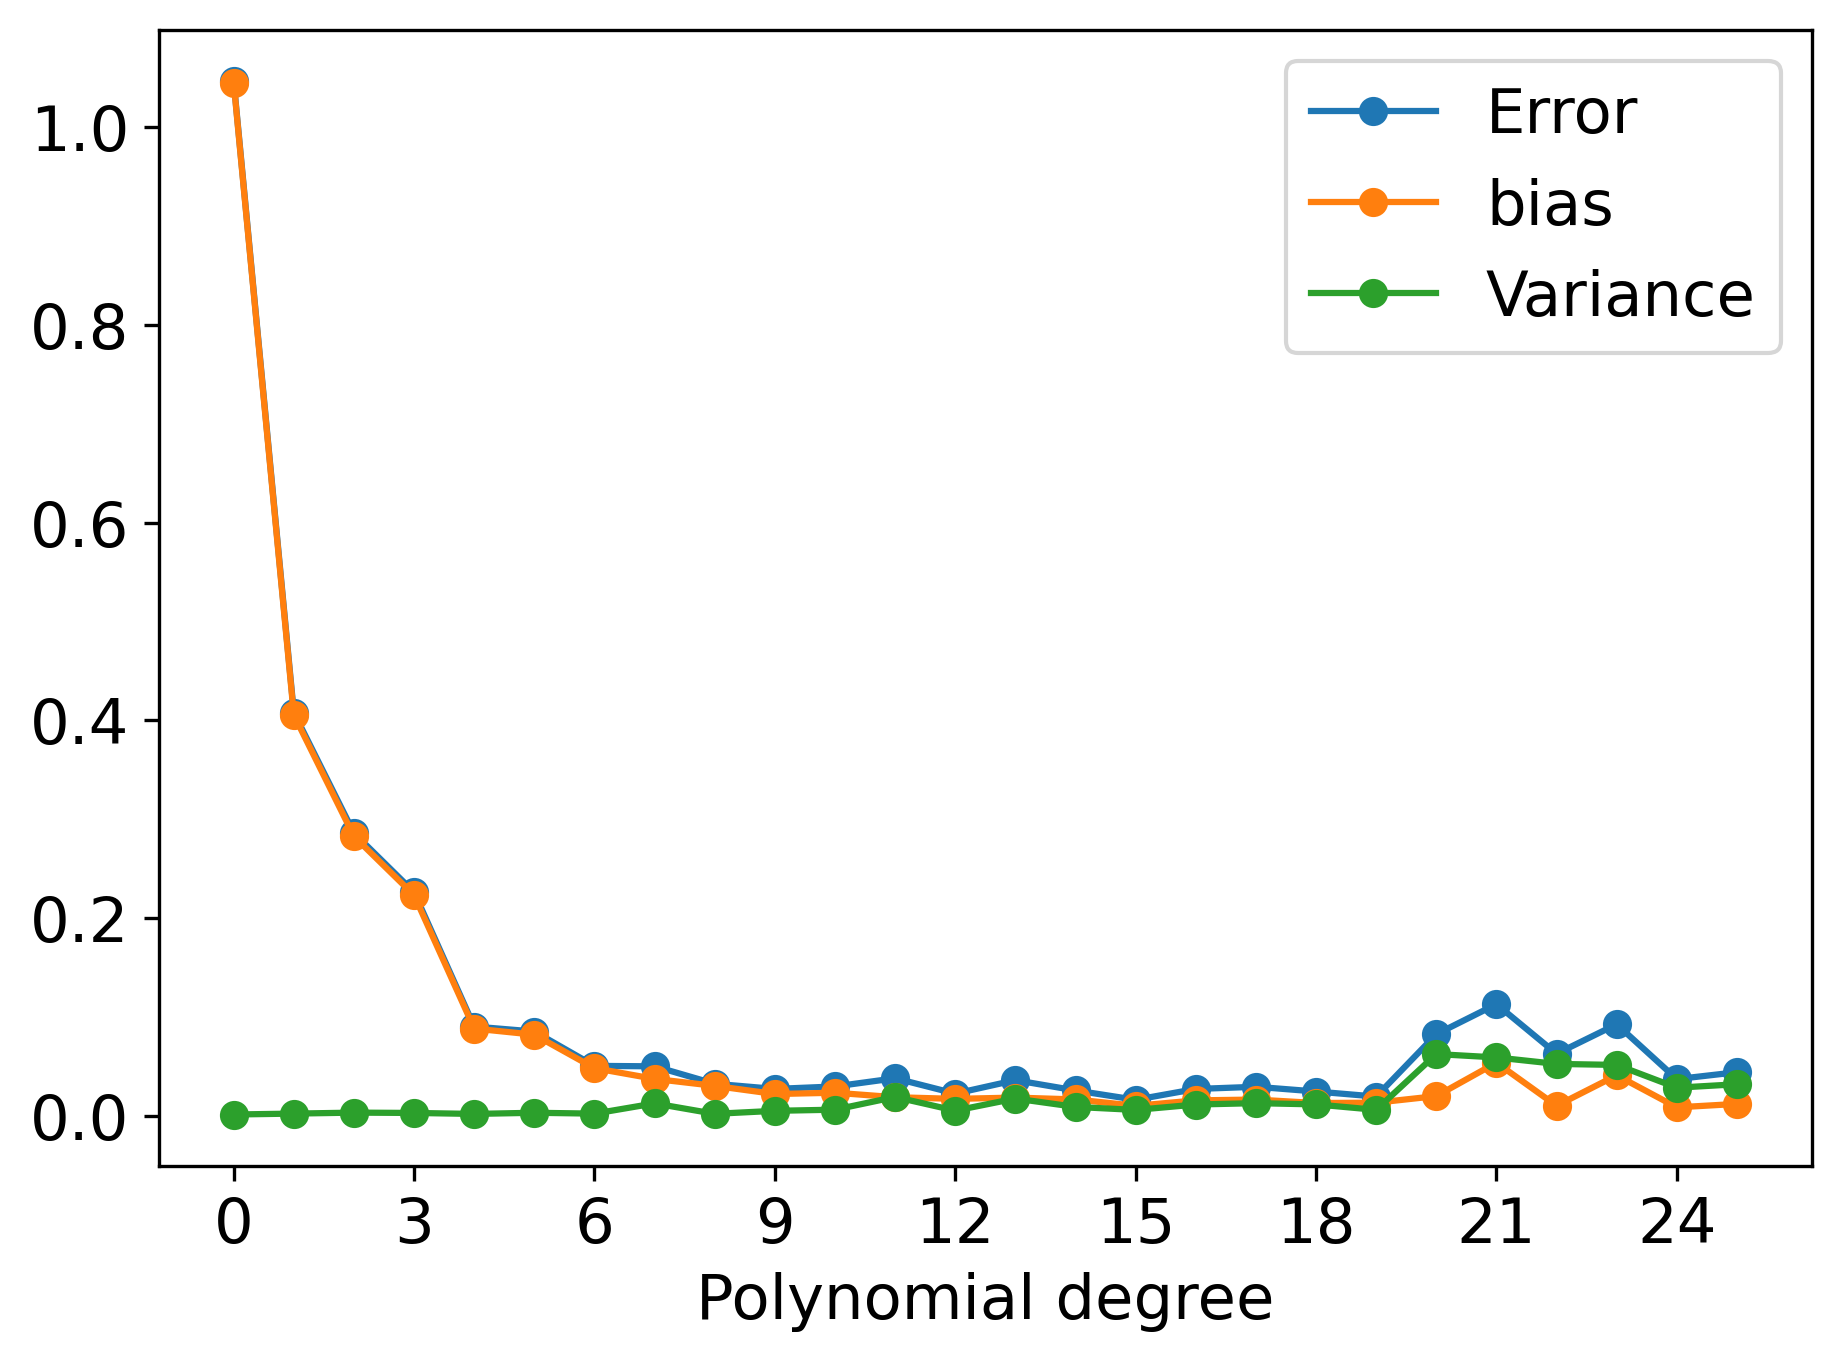
\includegraphics[width=.5\textwidth]{../figures/ols_real_tradeoff.png}
  \caption{Bias variance tradeoff for the OLS method}
  \label{fig:tradeoff_real}
\end{figure}

\begin{figure}[H]
  \begin{subfigure}{.5\textwidth}
    \centering
    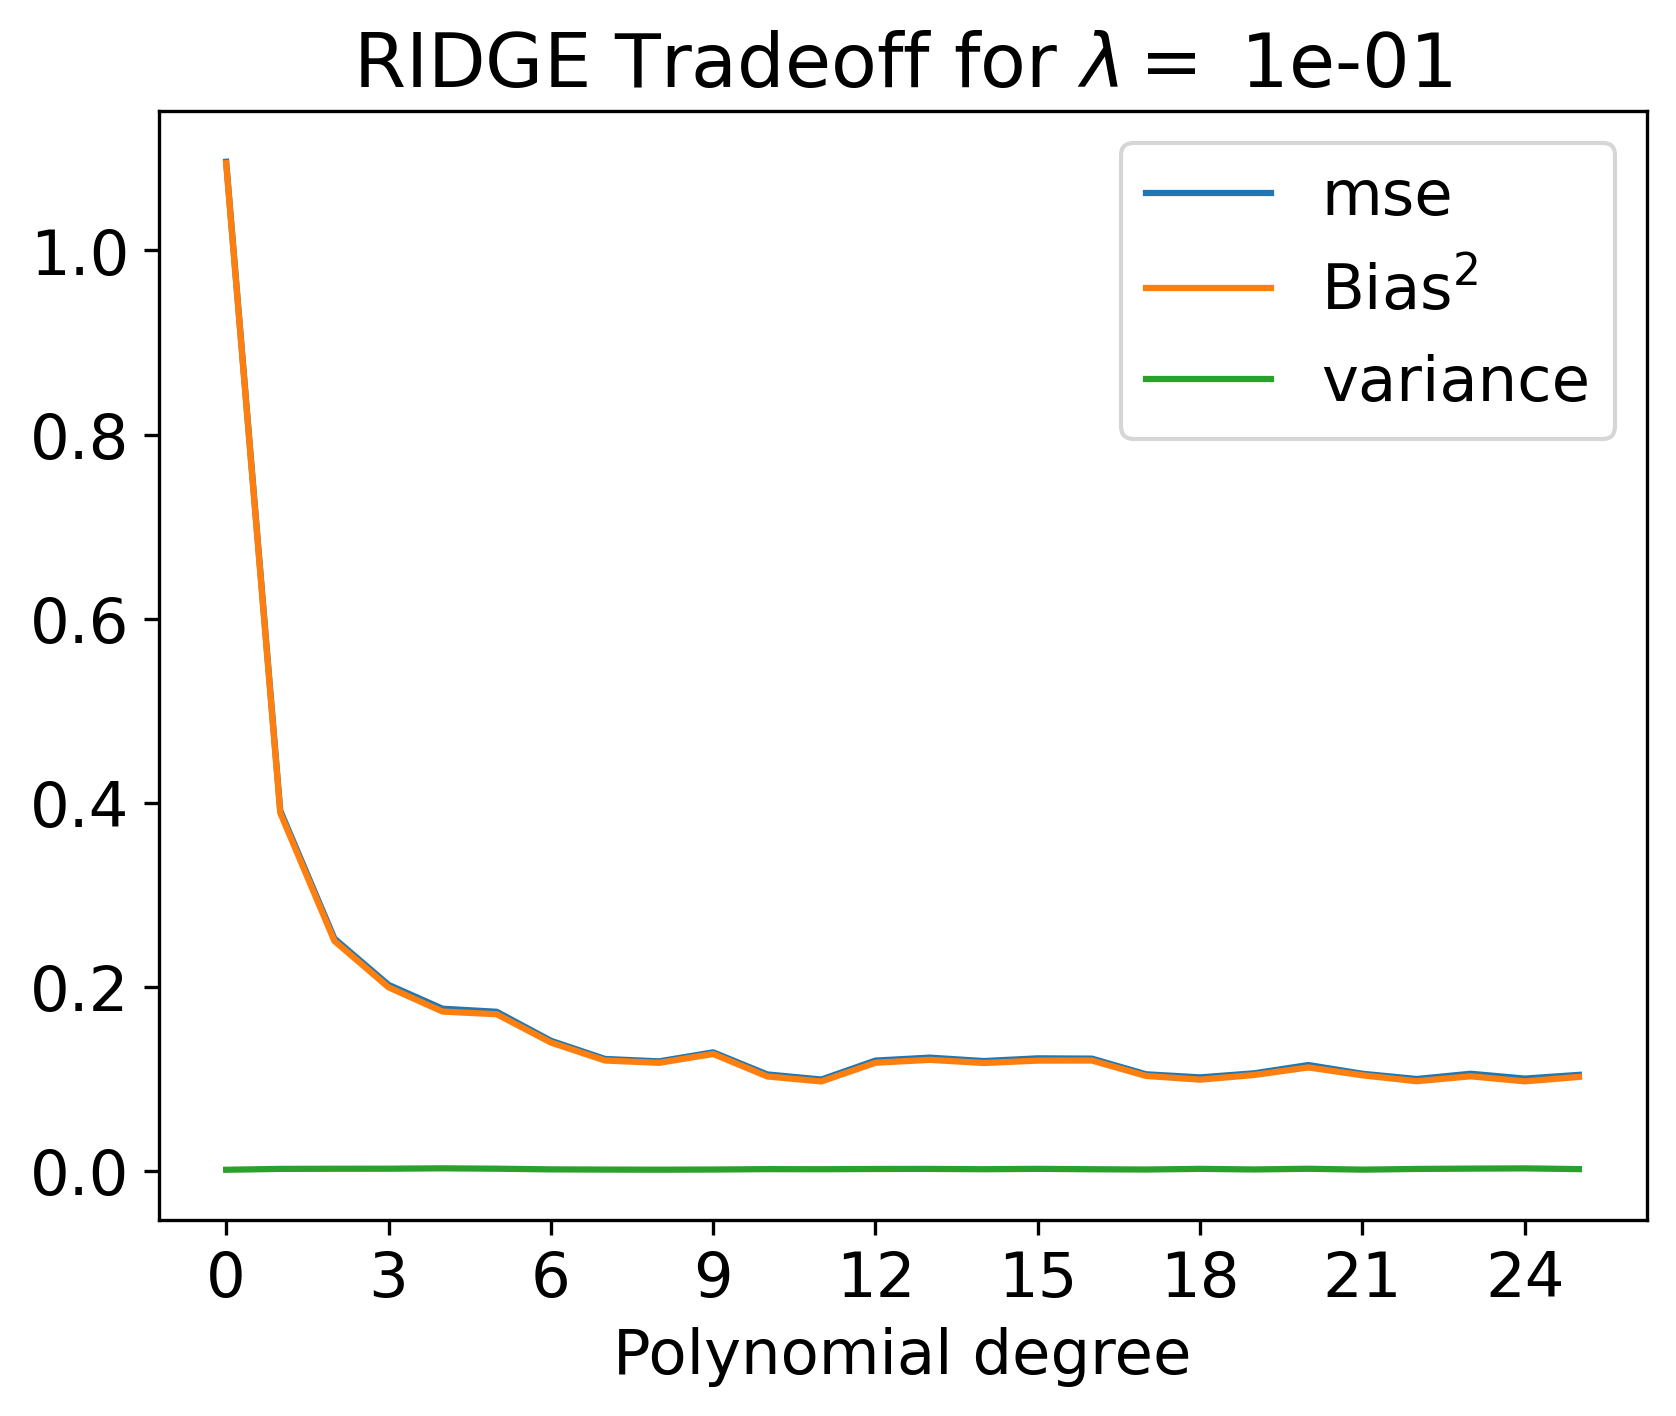
\includegraphics[width=\textwidth]{../figures/tradeoff_RIDGE_1e-01real.png}
    \caption{}
    \label{fig:}
  \end{subfigure}
  \begin{subfigure}{.5\textwidth}
    \centering
    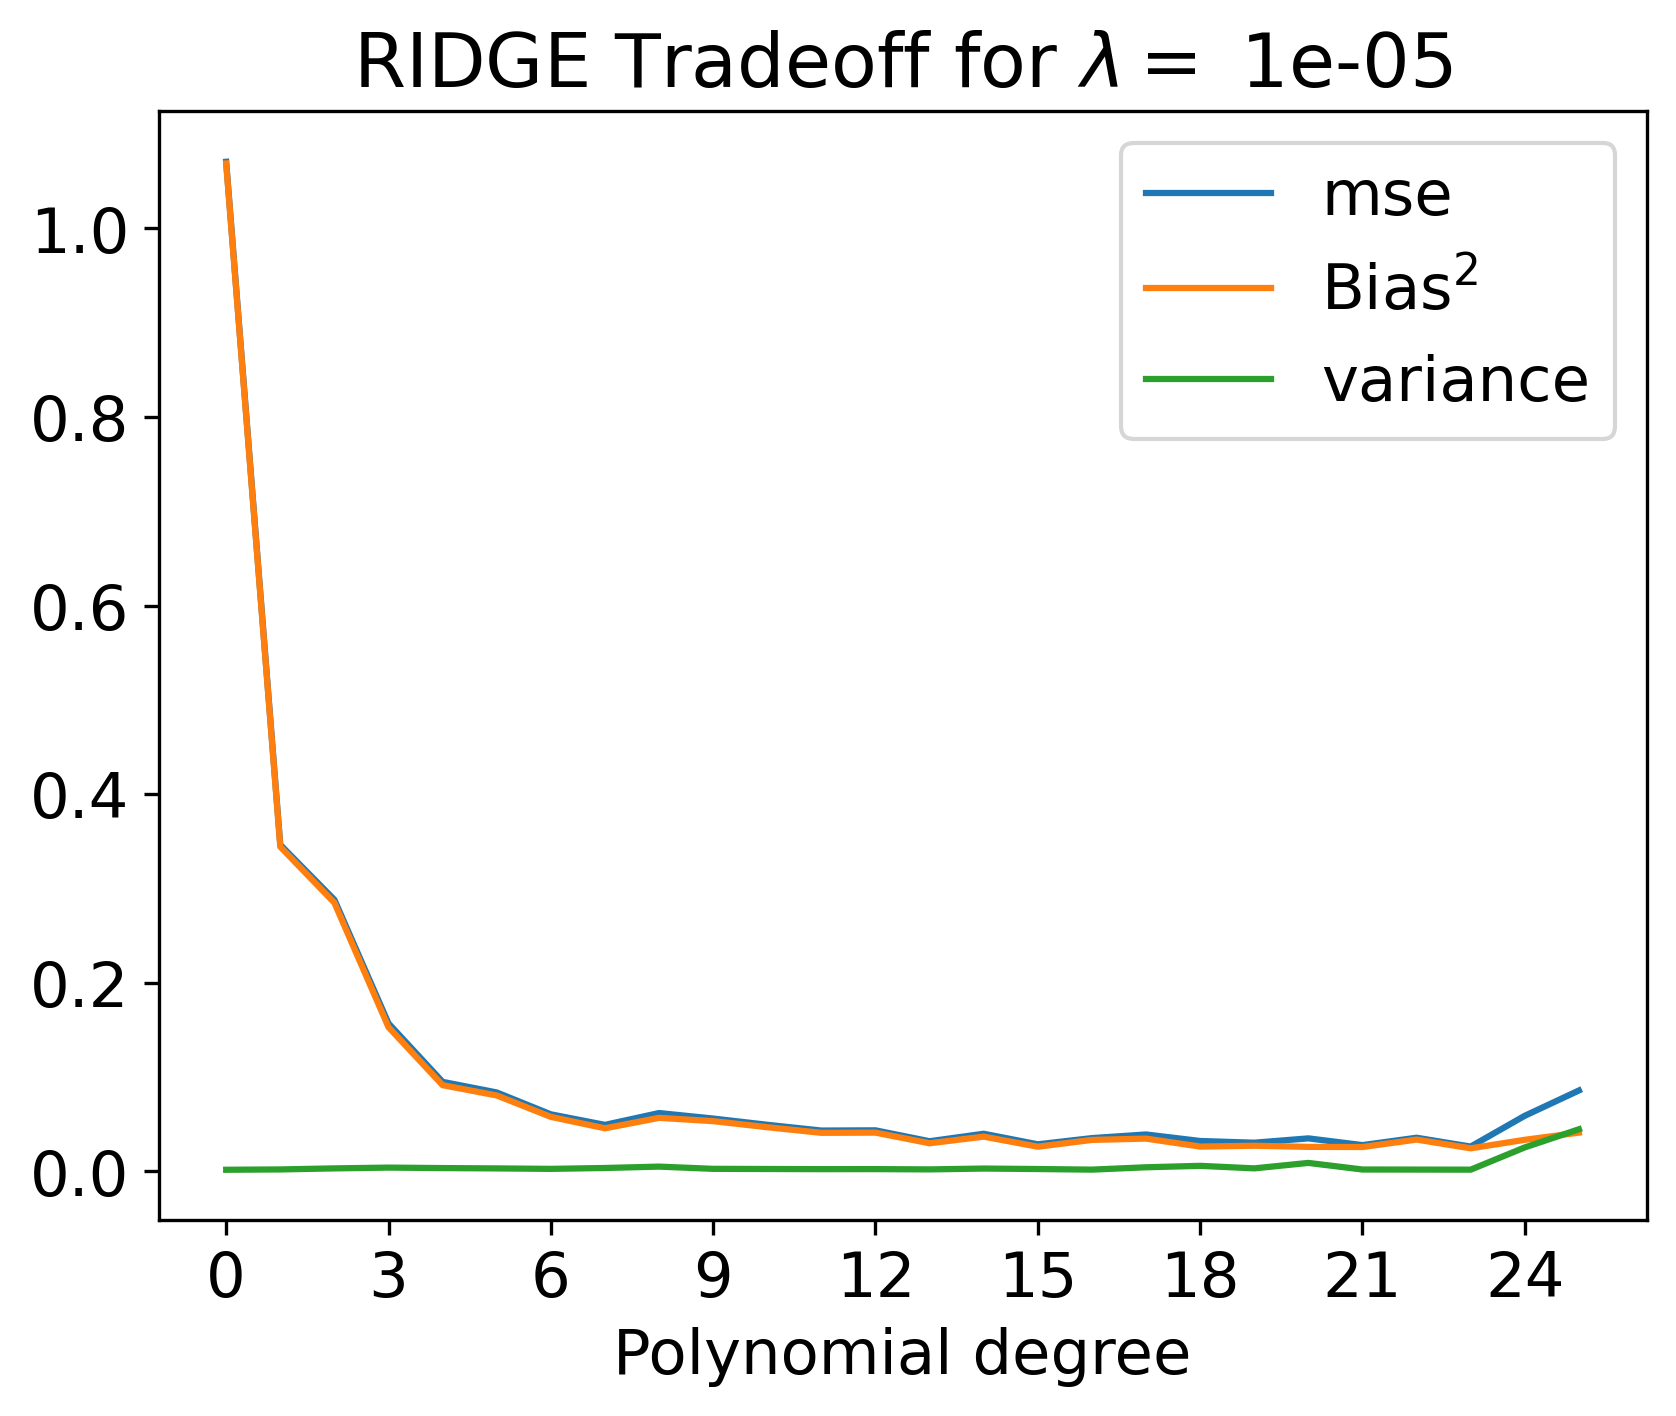
\includegraphics[width=\textwidth]{../figures/tradeoff_RIDGE_1e-05real.png}
    \caption{}
    \label{fig:}
  \end{subfigure}
  \begin{subfigure}{.5\textwidth}
    \centering
    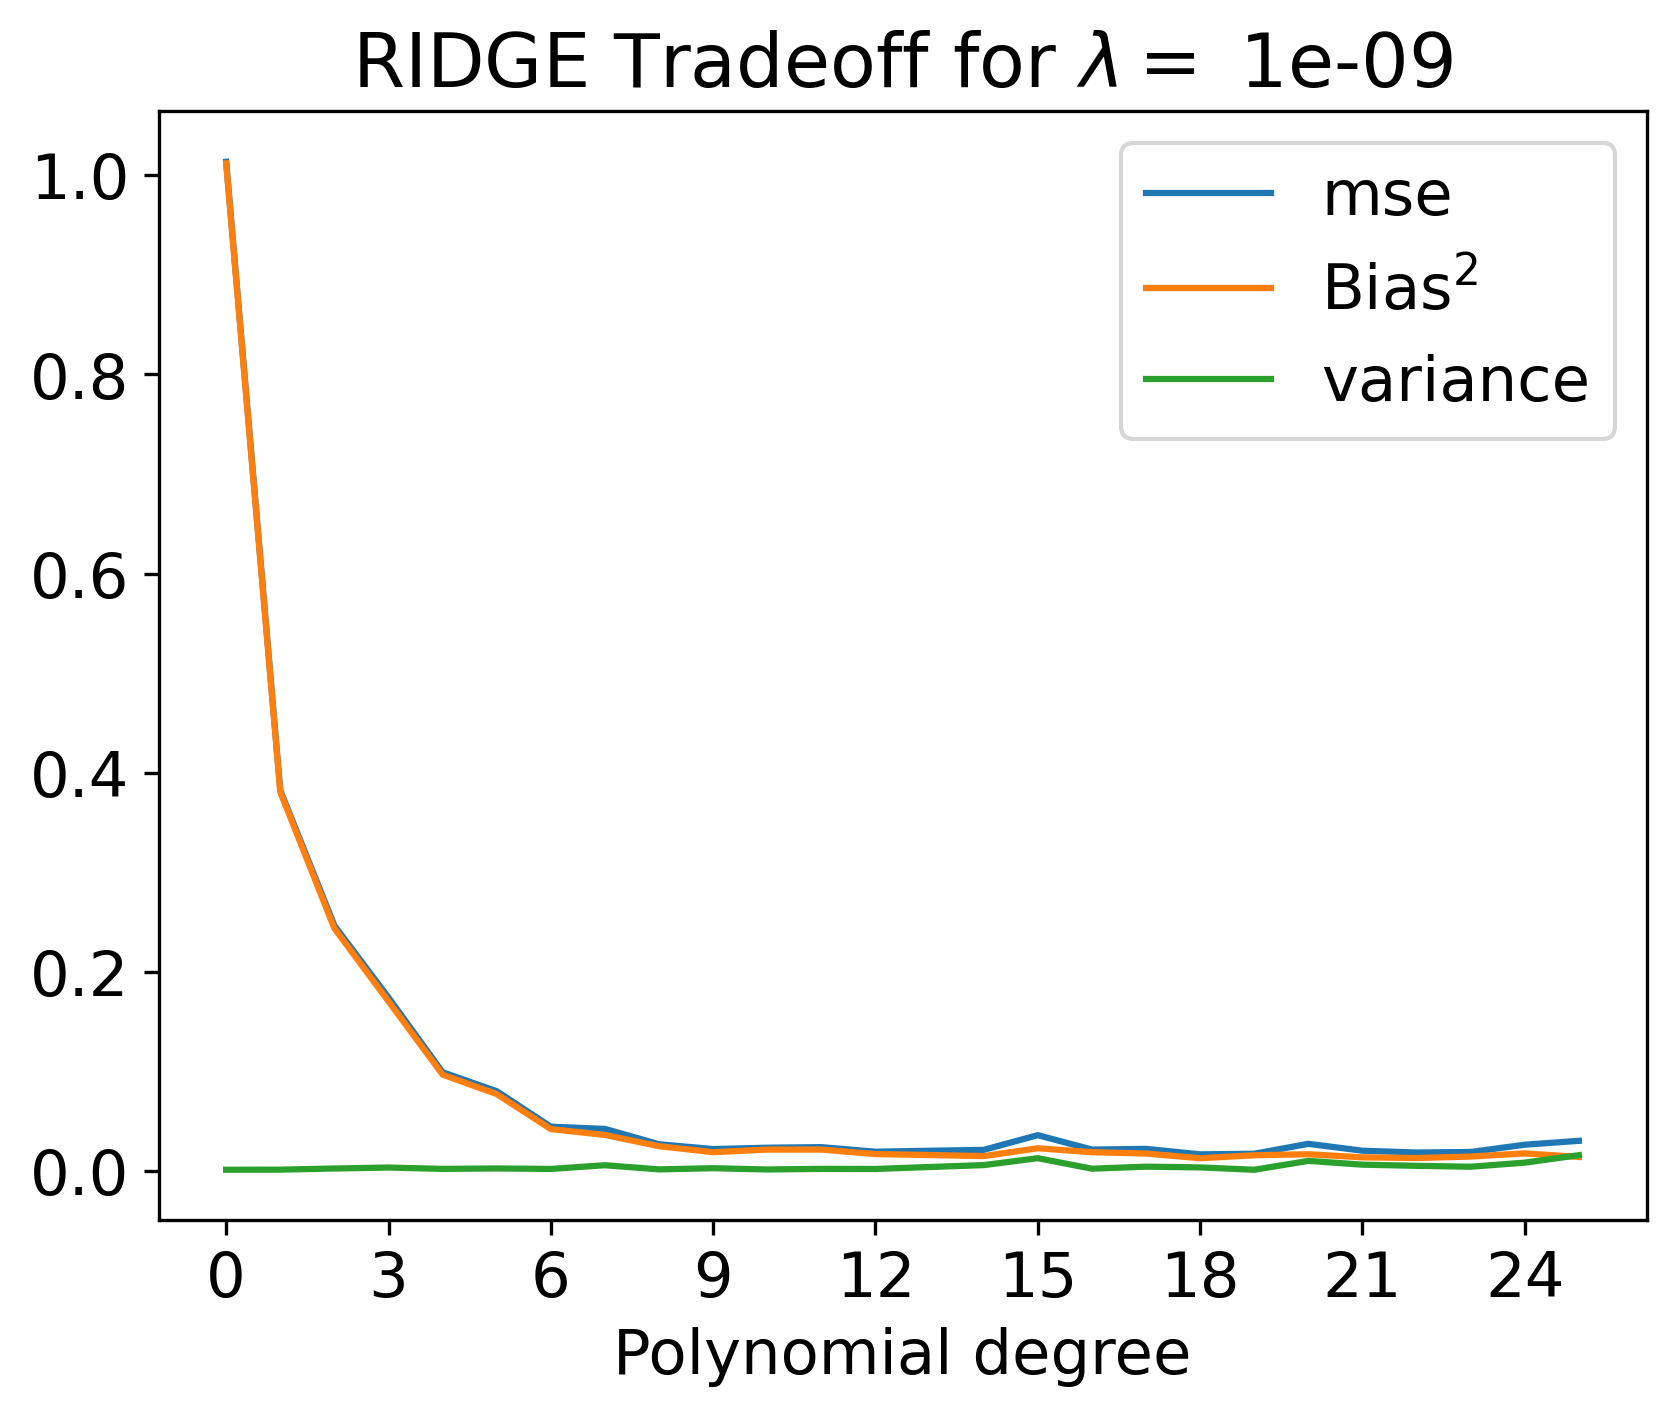
\includegraphics[width=\textwidth]{../figures/tradeoff_RIDGE_1e-09real.png}
    \caption{}
    \label{fig:}
  \end{subfigure}
  \begin{subfigure}{.5\textwidth}
    \centering
    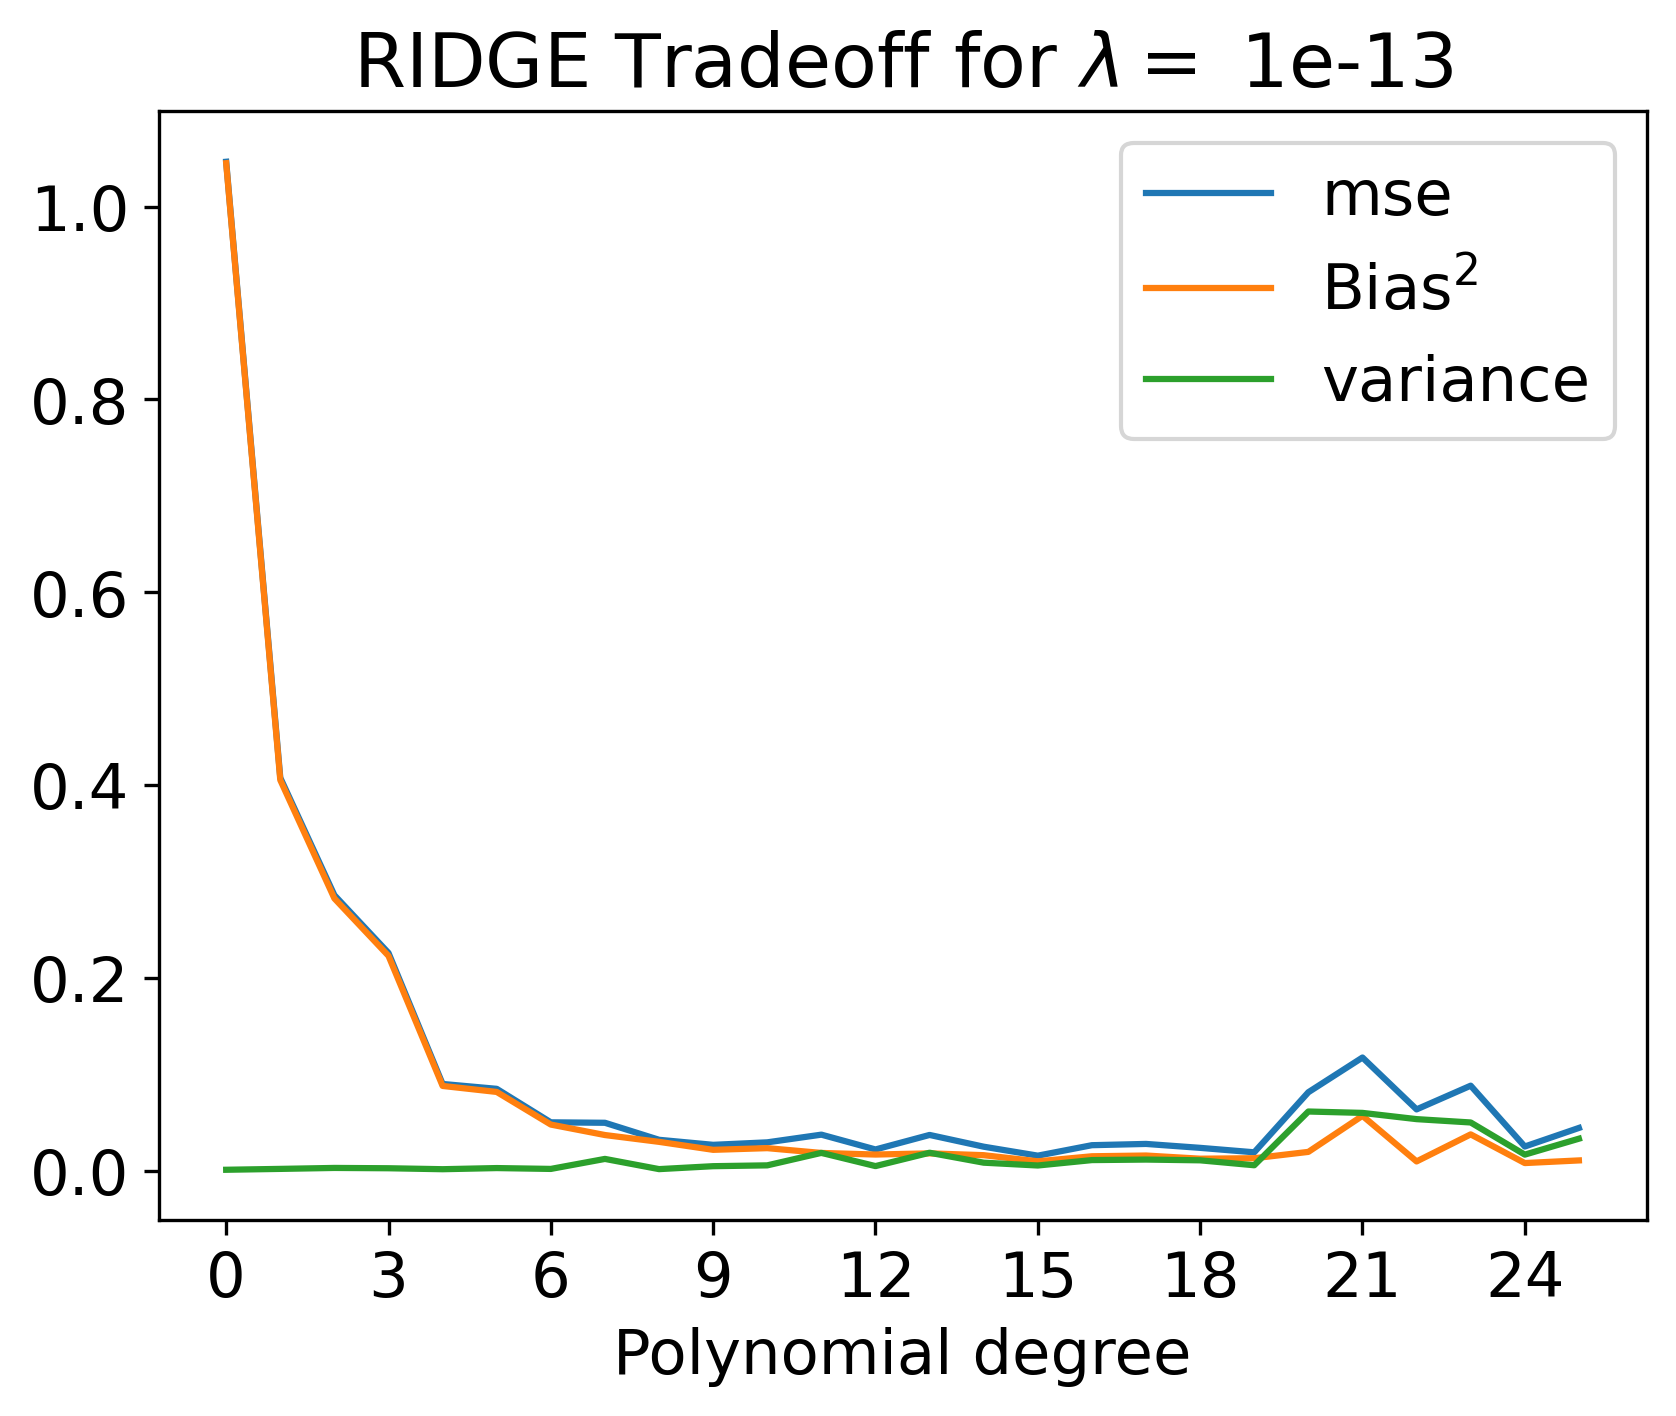
\includegraphics[width=\textwidth]{../figures/tradeoff_RIDGE_1e-13real.png}
    \caption{}
    \label{fig:}
  \end{subfigure}
  \caption{Bias variance tradeoff for different choices of lambda using Ridge regression}
  \label{fig:ridge_tradeoff_real}
\end{figure}

\begin{figure}[H]
  \begin{subfigure}{.5\textwidth}
    \centering
    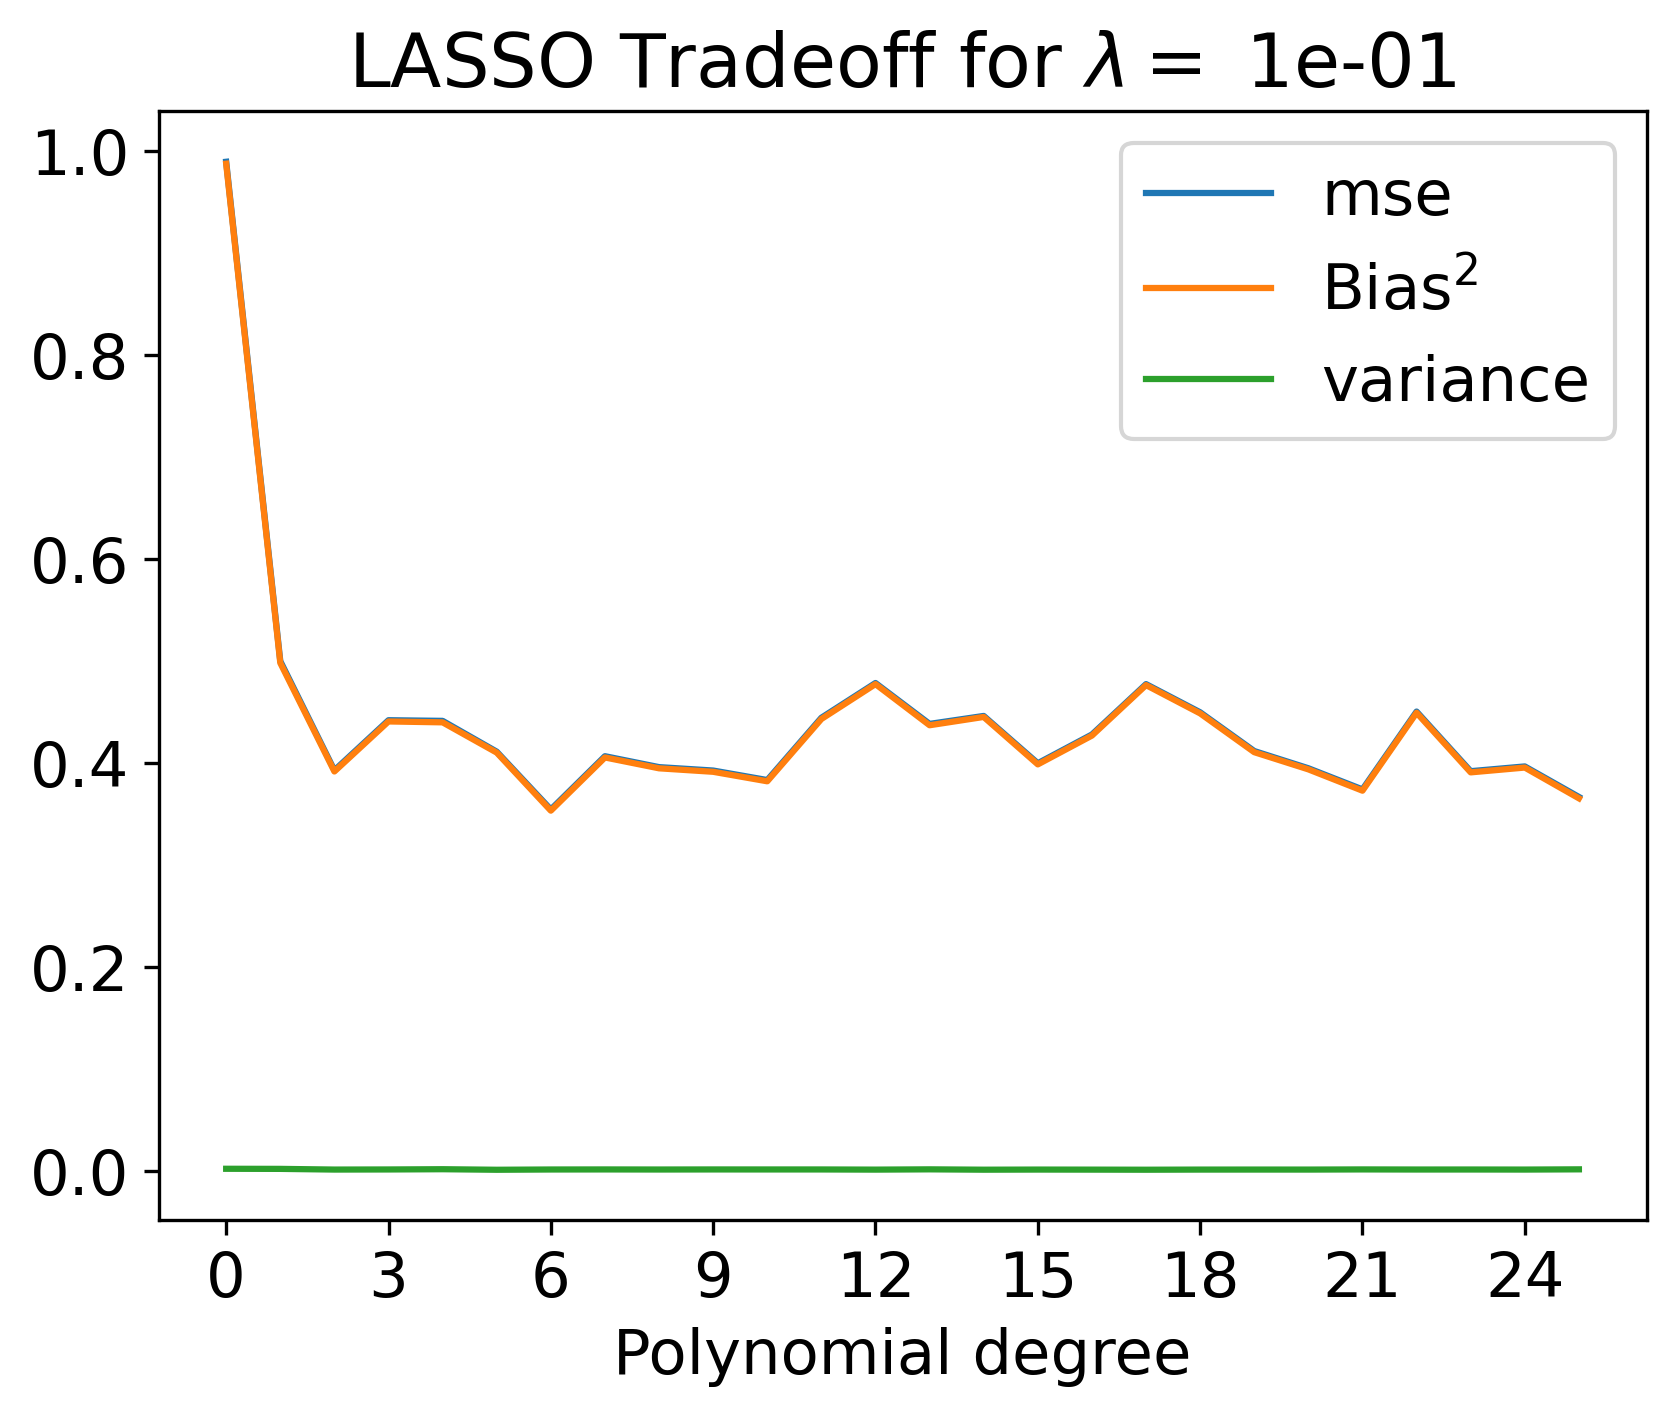
\includegraphics[width=\textwidth]{../figures/tradeoff_LASSO_1e-01real.png}
    \caption{}
    \label{fig:}
  \end{subfigure}
  \begin{subfigure}{.5\textwidth}
    \centering
    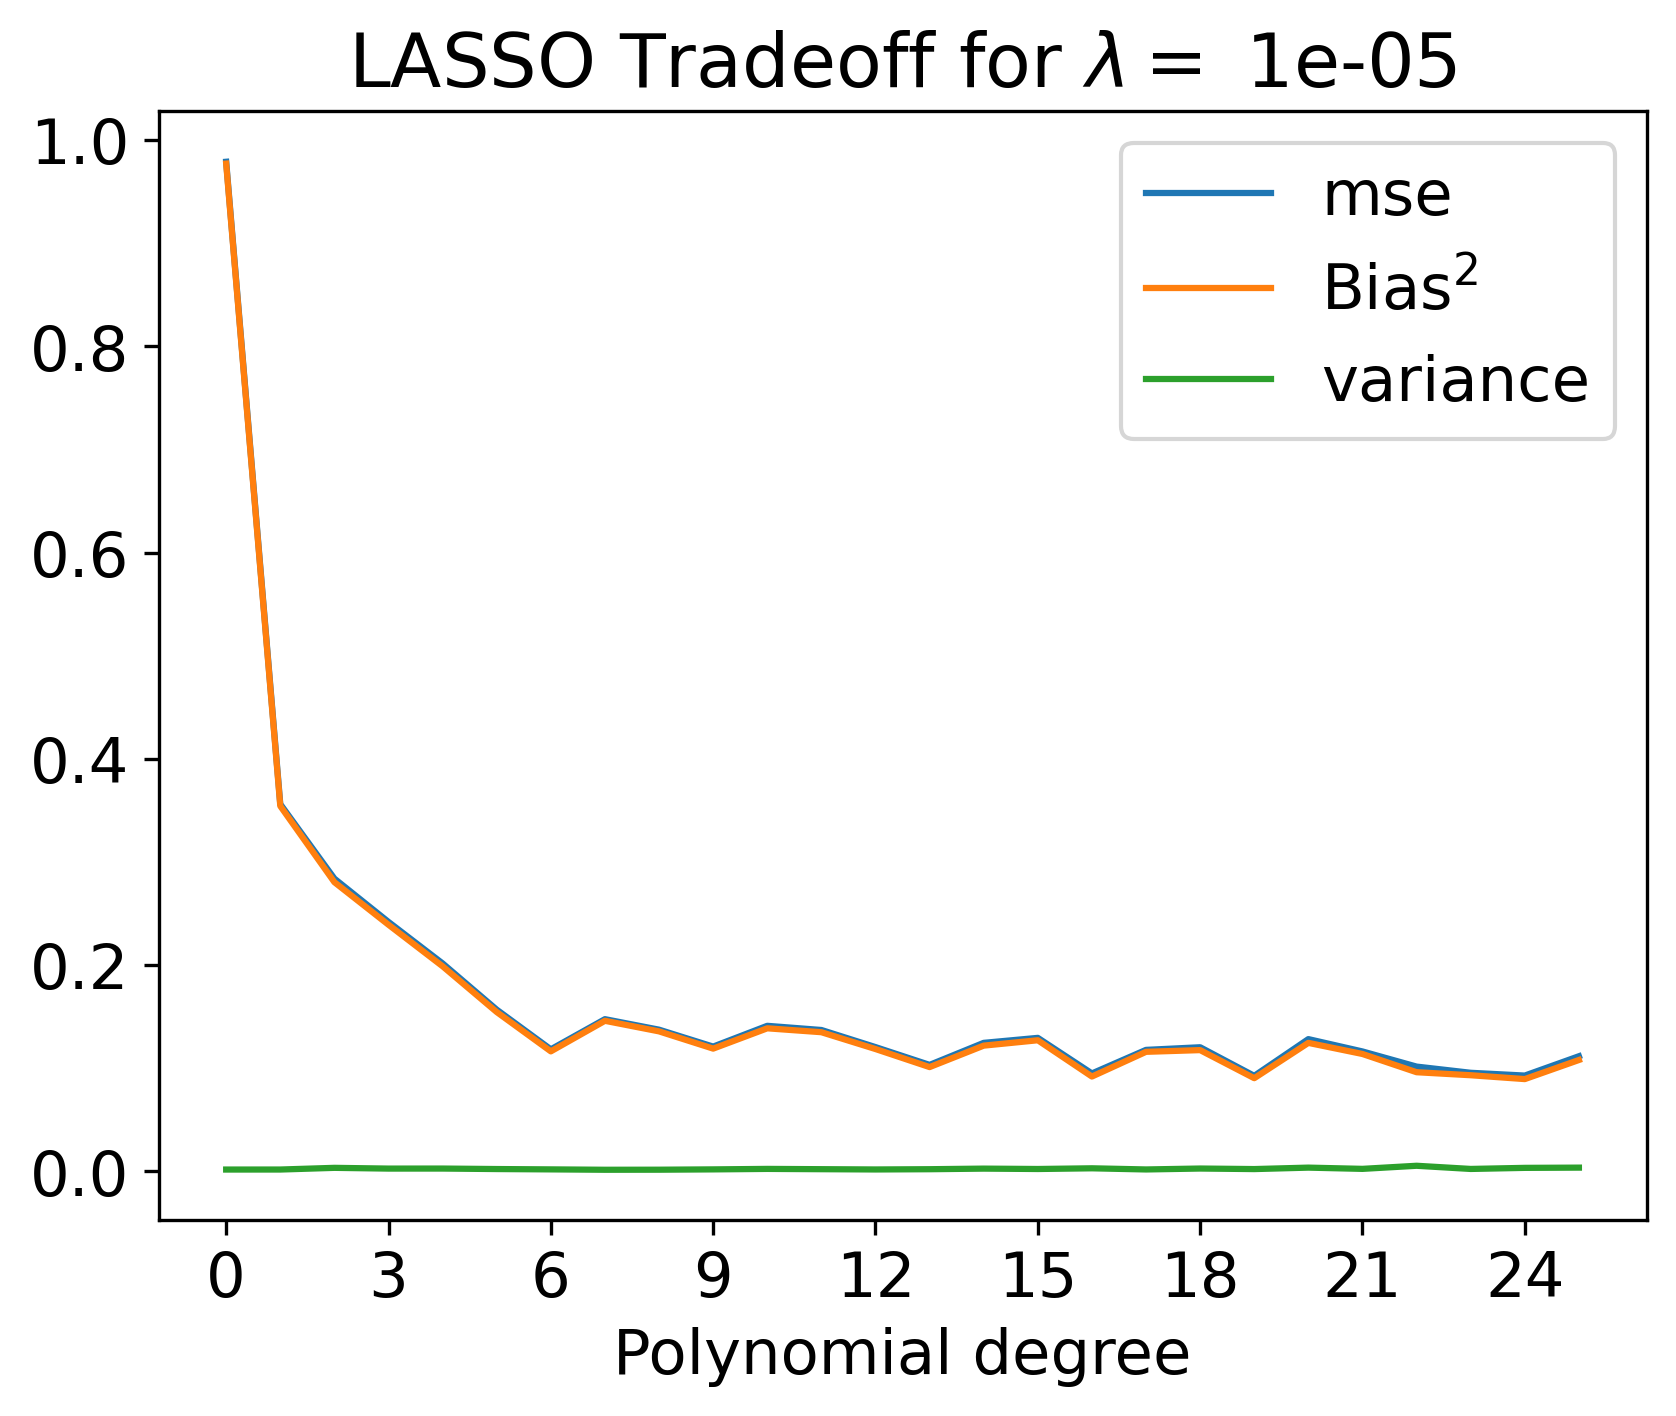
\includegraphics[width=\textwidth]{../figures/tradeoff_LASSO_1e-05real.png}
    \caption{}
    \label{fig:}
  \end{subfigure}
  \begin{subfigure}{.5\textwidth}
    \centering
    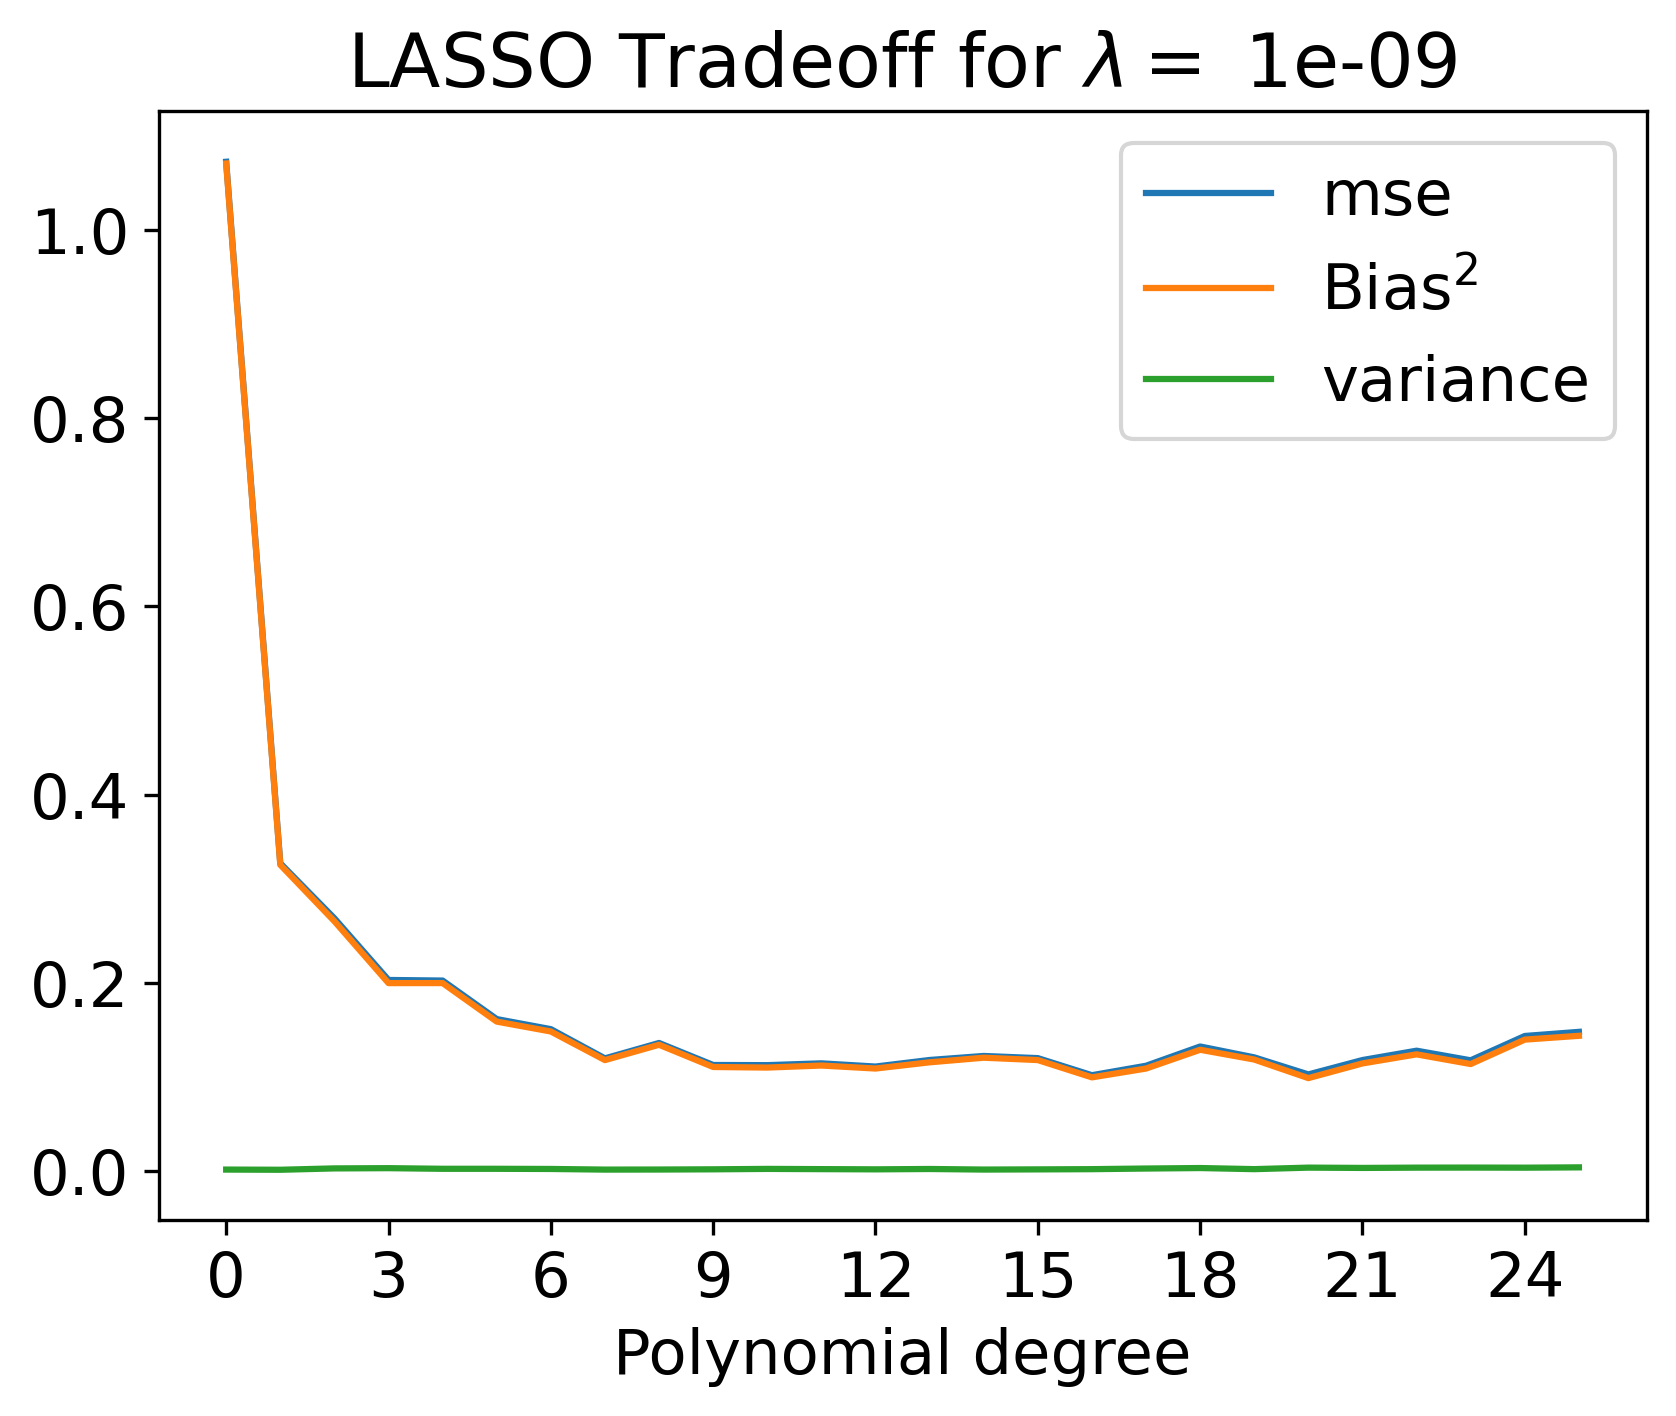
\includegraphics[width=\textwidth]{../figures/tradeoff_LASSO_1e-09real.png}
    \caption{}
    \label{fig:}
  \end{subfigure}
  \begin{subfigure}{.5\textwidth}
    \centering
    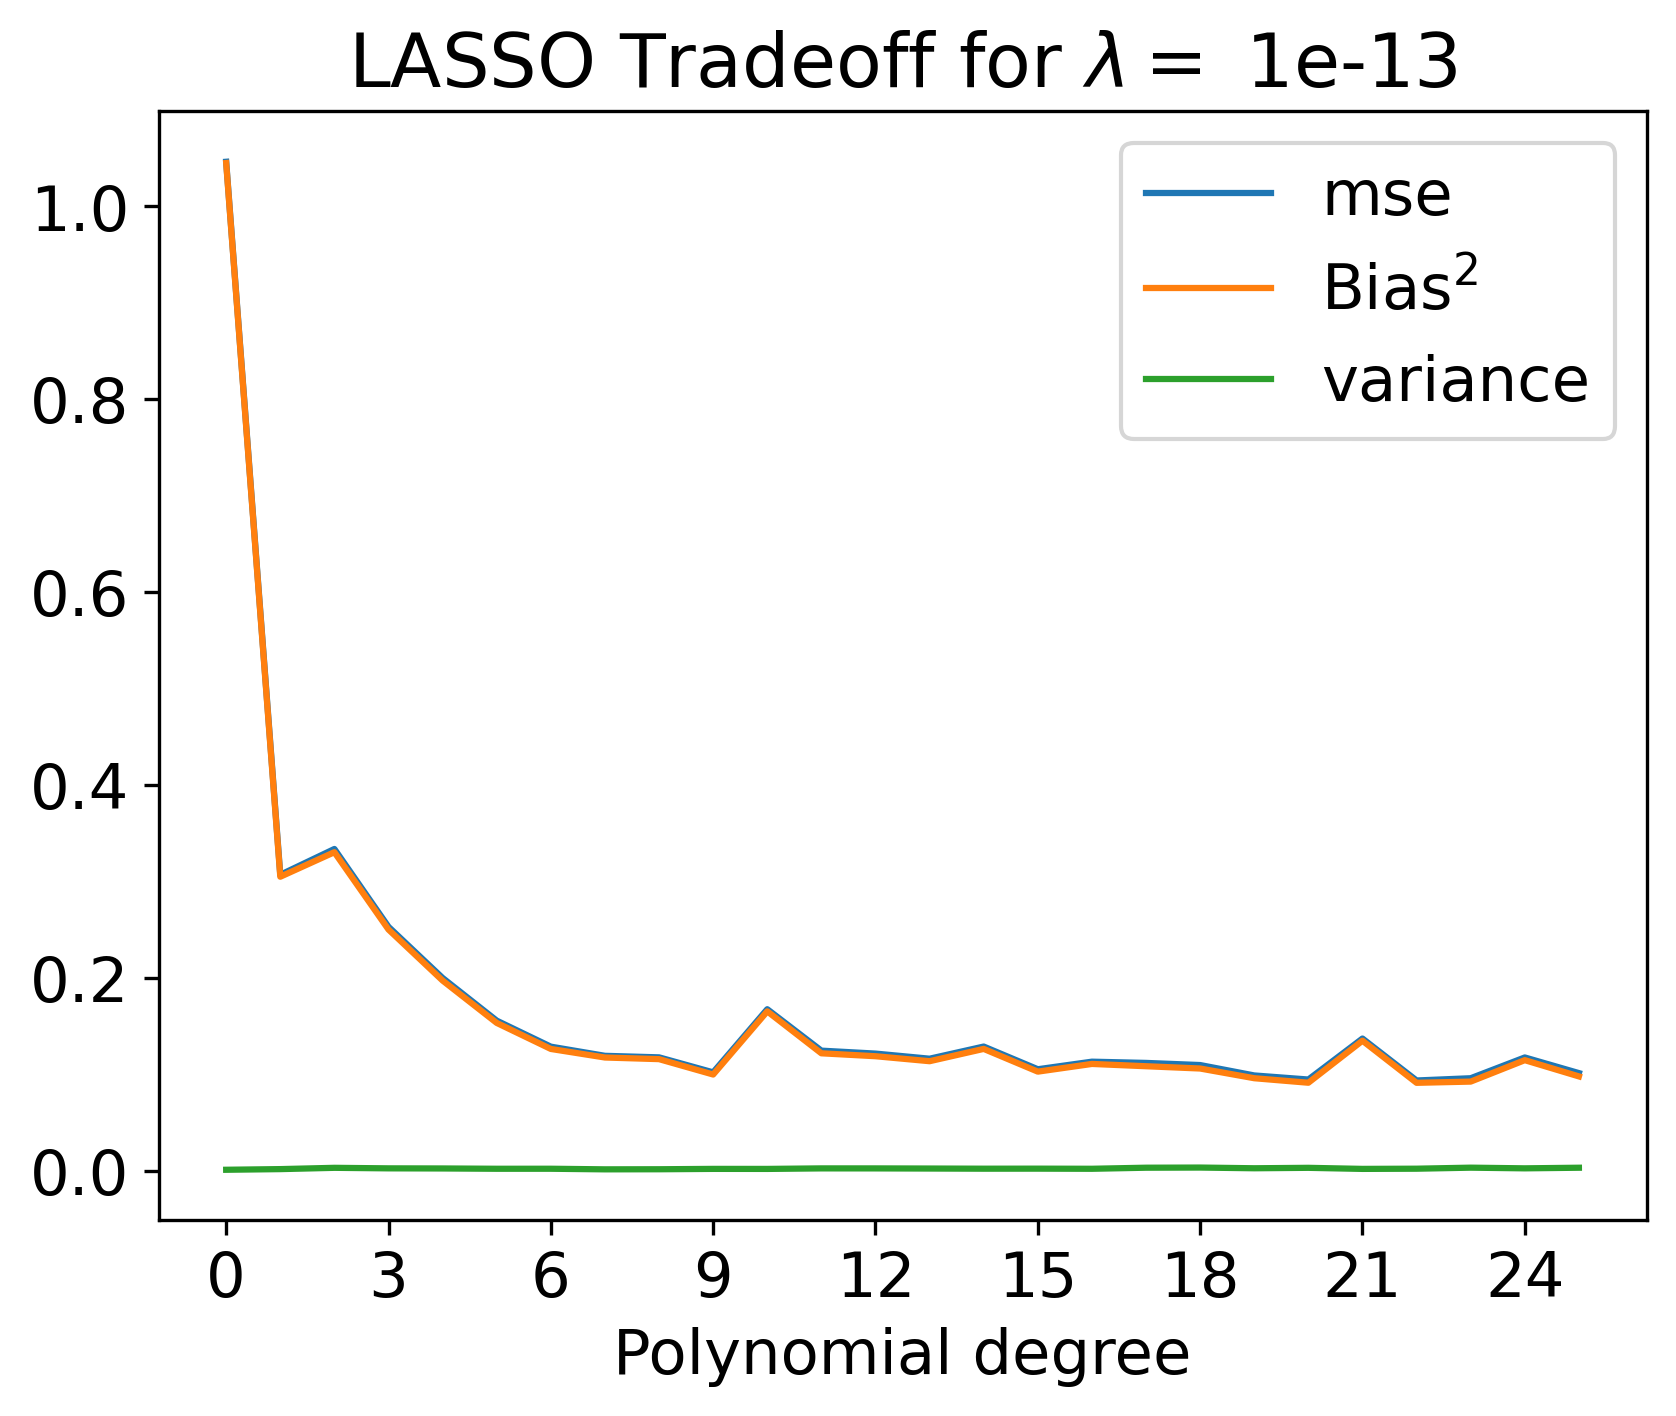
\includegraphics[width=\textwidth]{../figures/tradeoff_LASSO_1e-13real.png}
    \caption{}
    \label{fig:}
  \end{subfigure}
  \caption{Bias variance tradeoff for different choices of lambda using Ridge regression}
  \label{fig:lasso_tradeoff_real}
\end{figure}
We see that OLS keeps a low variance until a degree of 19 while the bias generally stays low for degrees of around 8 and above. For Ridge and Lasso we see the same trend as for OLS with a decreasing bias for greater degrees. On the other hand we do not notice any significant increase in the variance for both lasso and Ridge which more clearly can be seen in the OLS tradeoff. We also see that both Lasso and Ridge keeps a low variance up to a degree of 25 for different values of $\lambda$ which means that the bias has the main responsibility for the MSE of these models.

\subsection{Finding best models}

\begin{figure}
  \begin{subfigure}{\textwidth}
    \centering
    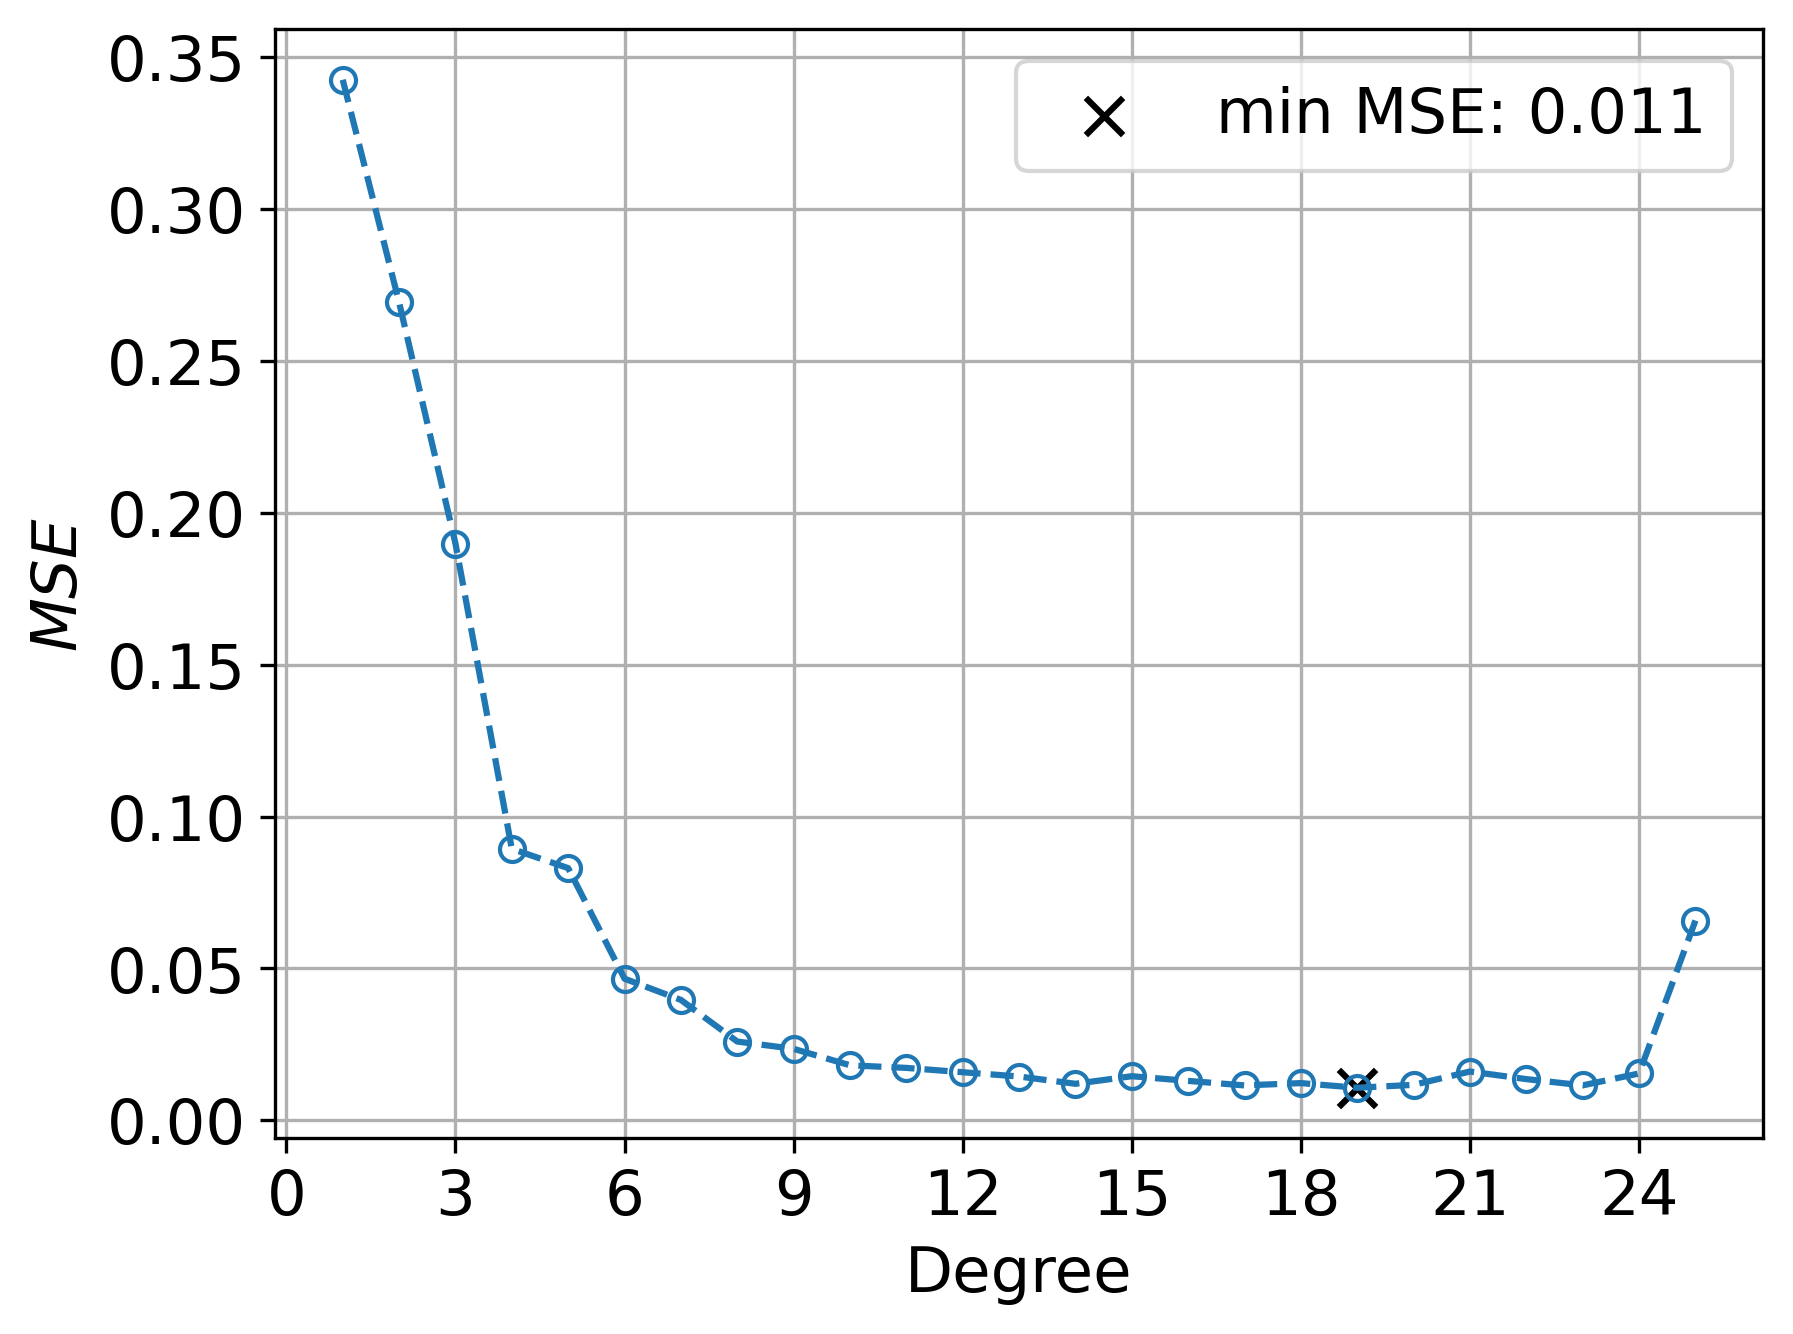
\includegraphics[width=\textwidth]{../figures/best_lambda_OLS_00.png}
    \caption{}
    \label{fig:}
  \end{subfigure}\\[1ex]
  \begin{subfigure}{.5\textwidth}
    \centering
    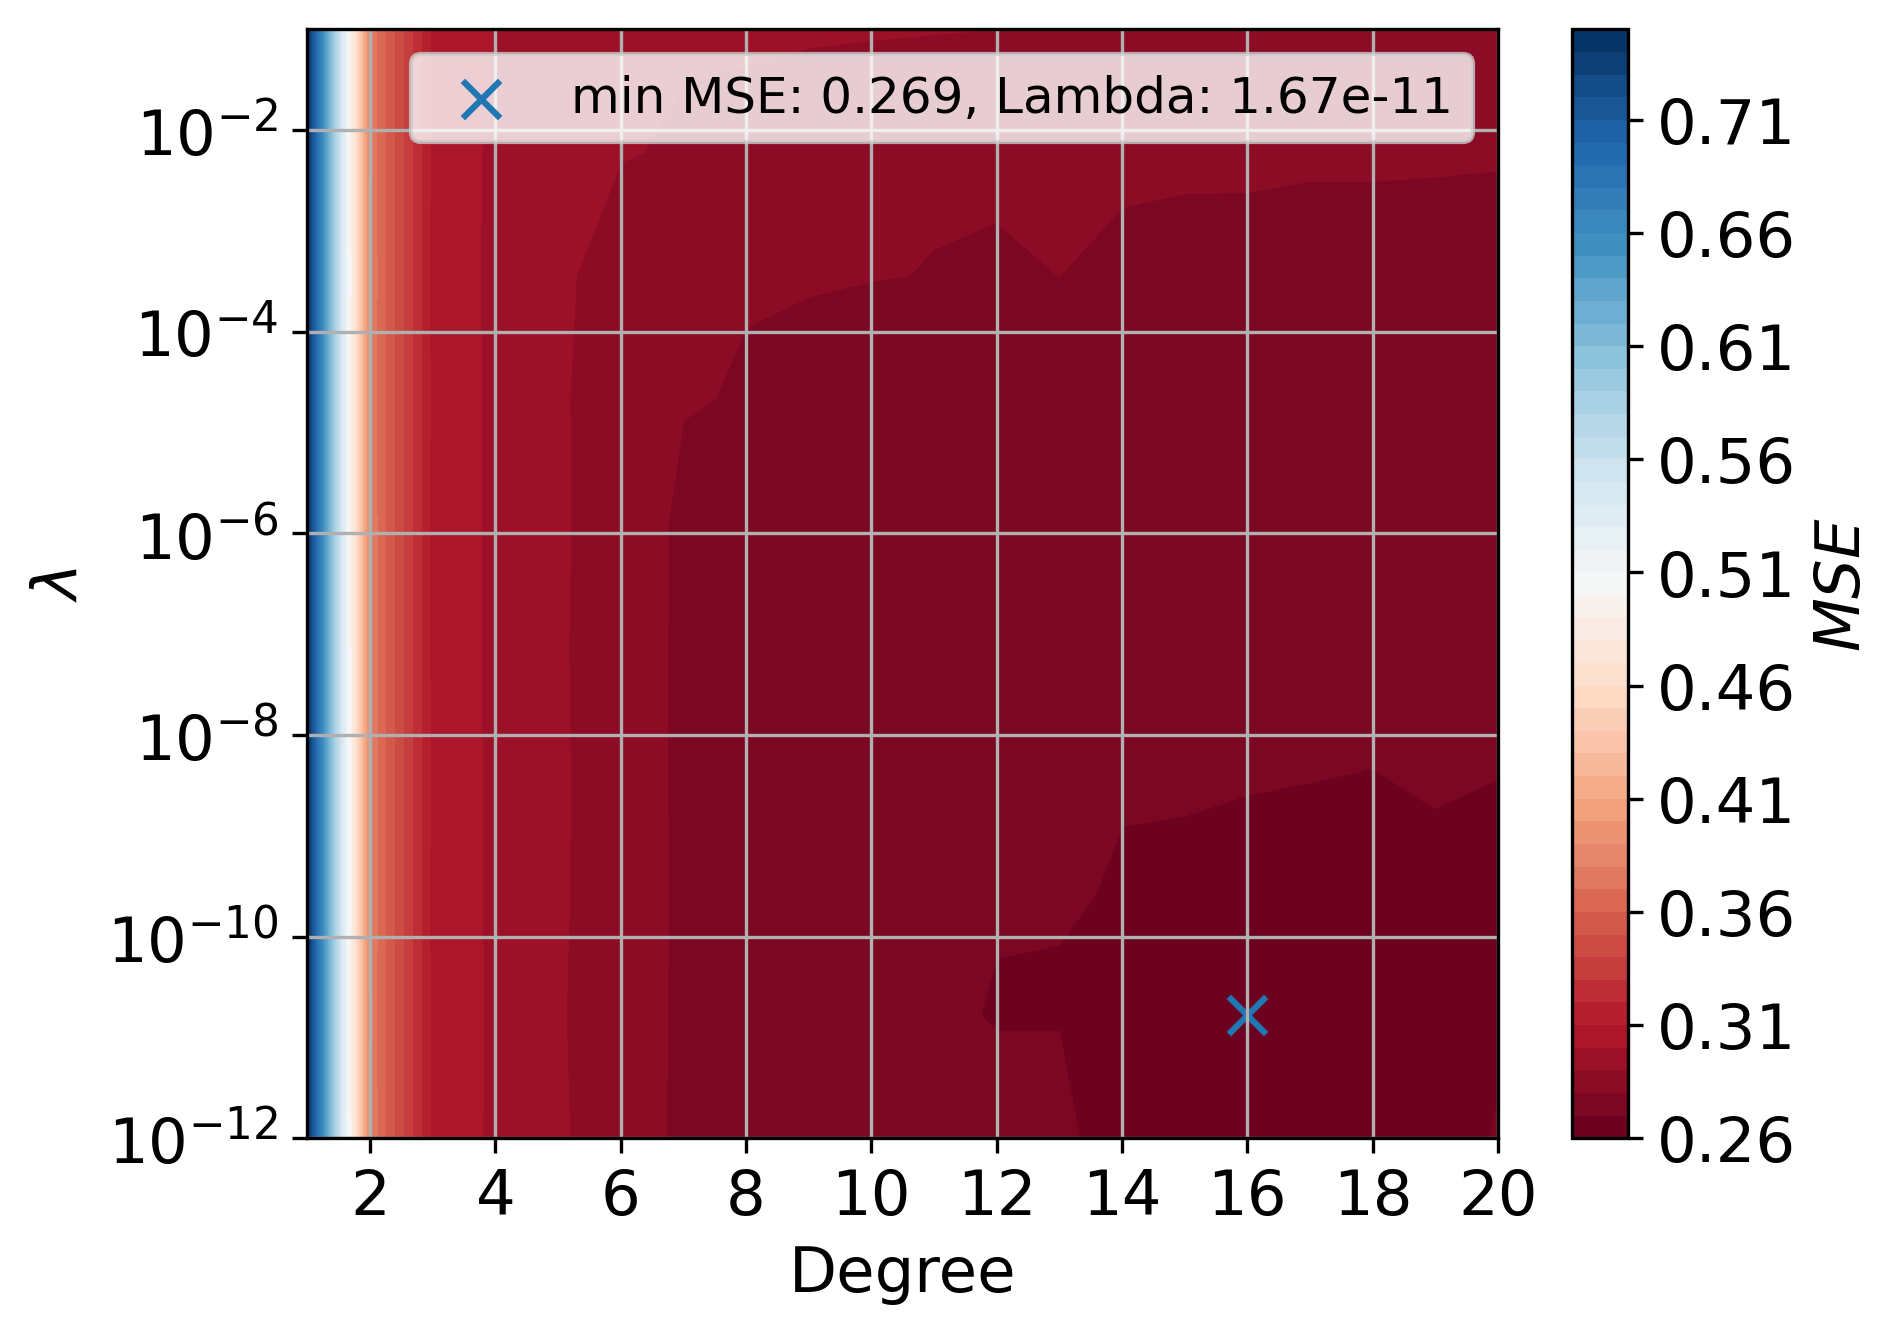
\includegraphics[width=\textwidth]{../figures/best_lambda_RIDGE_00.png}
    \caption{}
    \label{fig:}
  \end{subfigure}
  \begin{subfigure}{.5\textwidth}
    \centering
    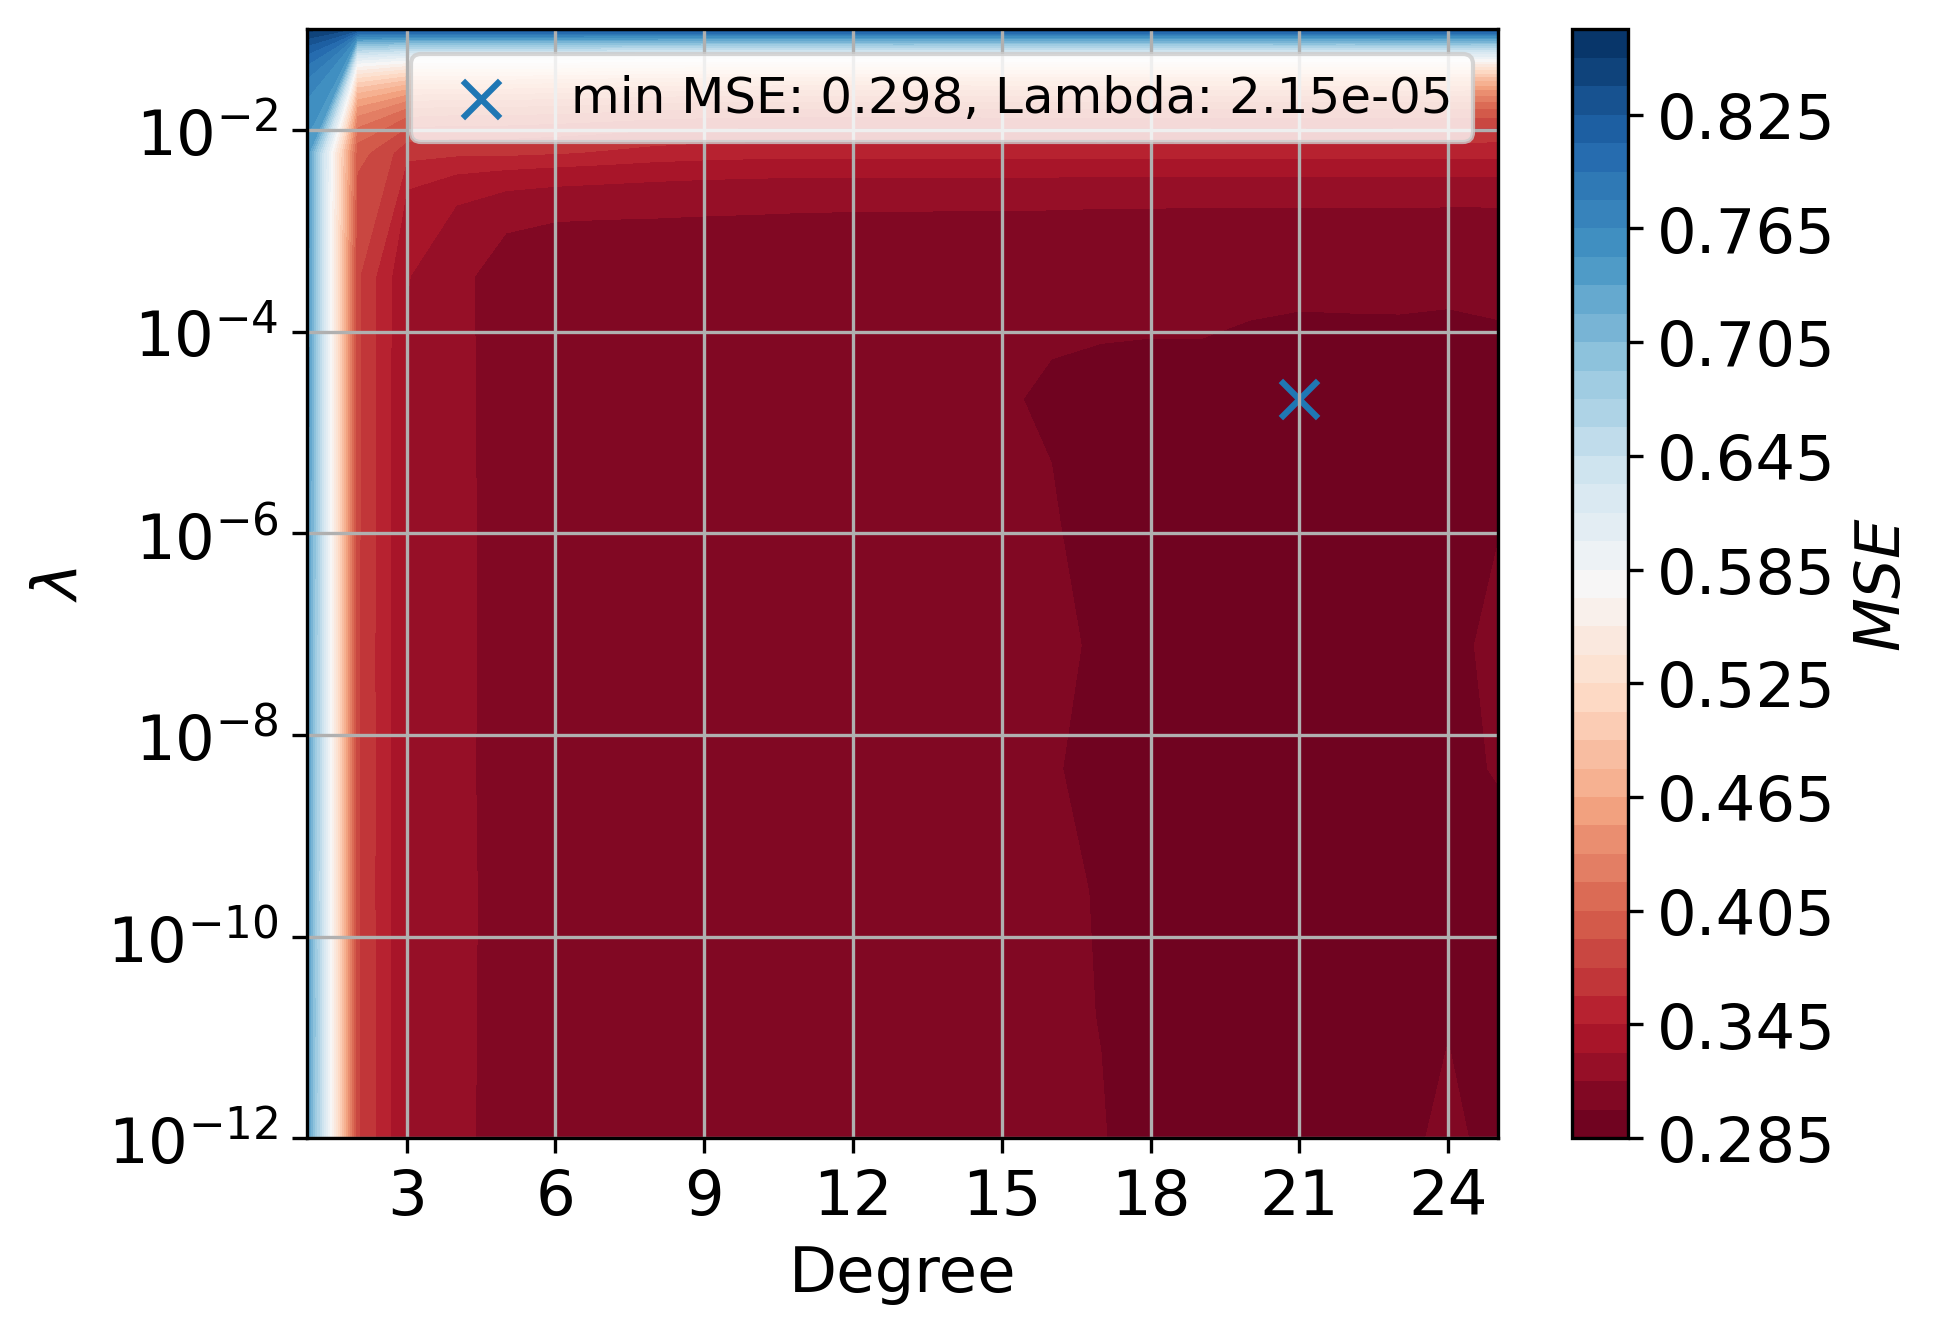
\includegraphics[width=\textwidth]{../figures/best_lambda_LASSO_00.png}
    \caption{}
    \label{fig:}
  \end{subfigure}
  \caption{Heatmap of MSE for different choices of polynomial degree and $\lambda$. Here we have used cross validation with 5$k$-folds for data of indexes [100:141] where every second index is skipped}
  \label{fig:heat_real}
\end{figure}
\section{Discussion}
\section{Conclusion}

\section{}

\end{document}
